\clearpage

\section{Efficiency Correction}
General idea.....

To obtain the real invariant mass spectrum of $D^0$ within STAR acceptance ($|\eta_{\pi}| \leq 1, |\eta_{K}| \leq 1, |Y_{K\pi}| \leq 1$), the raw spectrum should correct for the efficiency. The $K\pi$ pair efficiency within STAR acceptance is evaluated by folding the TPC related efficiency to the HFT related efficiency as shown on Eq.~\ref{effEqu}. For the TPC related tracking efficiency shows on the first term, we use STAR standard Full GEANT simulation. For the HFT related efficiency include the second and third terms which reflect to HFT acceptance and topological cuts, we developed the `Data-Driven Fast simulation' which will discuss later.

\begin{equation}
  \textup{Efficiency} \times \textup{Acceptance}  = \textup{TPC Tracking Eff} \otimes \textup{HFT Tracking Eff} \otimes \textup{Topollogy Cuts}
\label{effEqu}
\end{equation}

This formula can be written in another way when we consider the particles identification (PID) Eq.~\ref{effEqu2}. Here the PID part are able to factorized as Eq.~\ref{effEqu3}, Eq.~\ref{effEqu4}.

\begin{equation}
  \frac{\textup{HFT}}{\textup{MC}} =  \frac{\textup{TPC}_\textup{{withPID}}}{\textup{MC}} \otimes \frac{\textup{HFT}_\textup{{withPID}}}{\textup{TPC}_\textup{{withPID}}} \otimes \textup{PID}
\label{effEqu2}
\end{equation}

\begin{equation}
  \varepsilon(HFT \& PID_{TPC} \& PID_{TOF}) = \varepsilon(HFT | _{PID_{TPC} \& PID_{TOF}}) \times \varepsilon_{PID}(TPC\&TOF)
\label{effEqu3}
\end{equation}

\begin{equation}
  \varepsilon_{PID}(TPC\&TOF) = \varepsilon_{PID}(TOF | TPC) \times \varepsilon_{TPC}
\label{effEqu4}
\end{equation}

\subsection{Single Track Efficiency}

The single track efficiency losses have two contributions, the detector inefficiency and particle identification cuts. The detector efficiency includes the TPC tracking efficiency ($\varepsilon_{TPC}$) and the TOF matching efficiency ($\varepsilon_{TOF}$). The particle identification cut efficiency ($\varepsilon_{PID}$) includes the efficiencies of TOF velocity (1/$\beta$) and the $dE/dx$ selection cuts. So the single track efficiency can be derived by the Eq.~\ref{singleeff}

\begin{equation}
\varepsilon = \varepsilon_{TPC} \times \varepsilon_{TOF} \times \varepsilon_{PID}
\label{singleeff}
\end{equation}

\subsection{TPC Tracking Efficiency}

The TPC tracking efficiency ($\varepsilon_{TPC}$) is evaluated via the standard STAR embedding technique. TPC efficiency including two parts, TPC response and acceptance efficiency. The Monte Carlo (MC) tracks are embedded into the raw data to have a realistic detector occupancy environment. The raw data is randomly sampled over the entire Au+Au minimum-bias data set, while the number of embedded MC tracks is constrained to 5\% of the measured multiplicity of the real events to avoid a sizable impact on the realistic TPC tracking efficiency. The MC tracks, with flat $p_{T}$, $\eta$, and $\phi$, are generated and passed through the full GEANT simulation of the STAR detector geometry, and then mixed with the real data . The mixed signals are processed using the same procedures as real data.  The quality assurance is made to ensure the MC simulation reproduces the real data before studying the TPC tracking efficiency (Embedding QA). The TPC tracking efficiency is derived by taking the ratio of the number of reconstructed MC tracks ($N_{rec}$), satisfying the track quality cuts used in the data analysis, over the number of embedded MC tracks ($N_{emb}$), as shown in Eq.~\ref{tpceff}

\begin{equation}
\varepsilon_{TPC} = \frac{N_{rec}\;(nHitsFit\geq20\;\&\;dca\leq1\;\&\;|\eta|\leq1\;\&\;nCommonHits > 10)}{N_{emb}\;(|\eta|\leq1)}
\label{tpceff}
\end{equation}

The TPC tracking efficiency in Run14 Au+Au collisions at 200 GeV is shown below. Fig ~\ref{fig:mpion} shows the TPC tracking efficiency for pion plus from four different classifications, from up to down, the centrality is from the most peripheral to most central collision. As we see, in the most central top 0-5\% collisions, due to the large occupancy the TPC tracking efficiency is much lower than the central one. Fig. ~\ref{fig:mkaon} shows the same plot for kaon minus. The Kaon can be decay inside TPC, that's the reason the TPC tracking efficiency is lower than pion.

\begin{figure}[htbp]
\begin{minipage}[htbp]{0.52\linewidth}
\centering
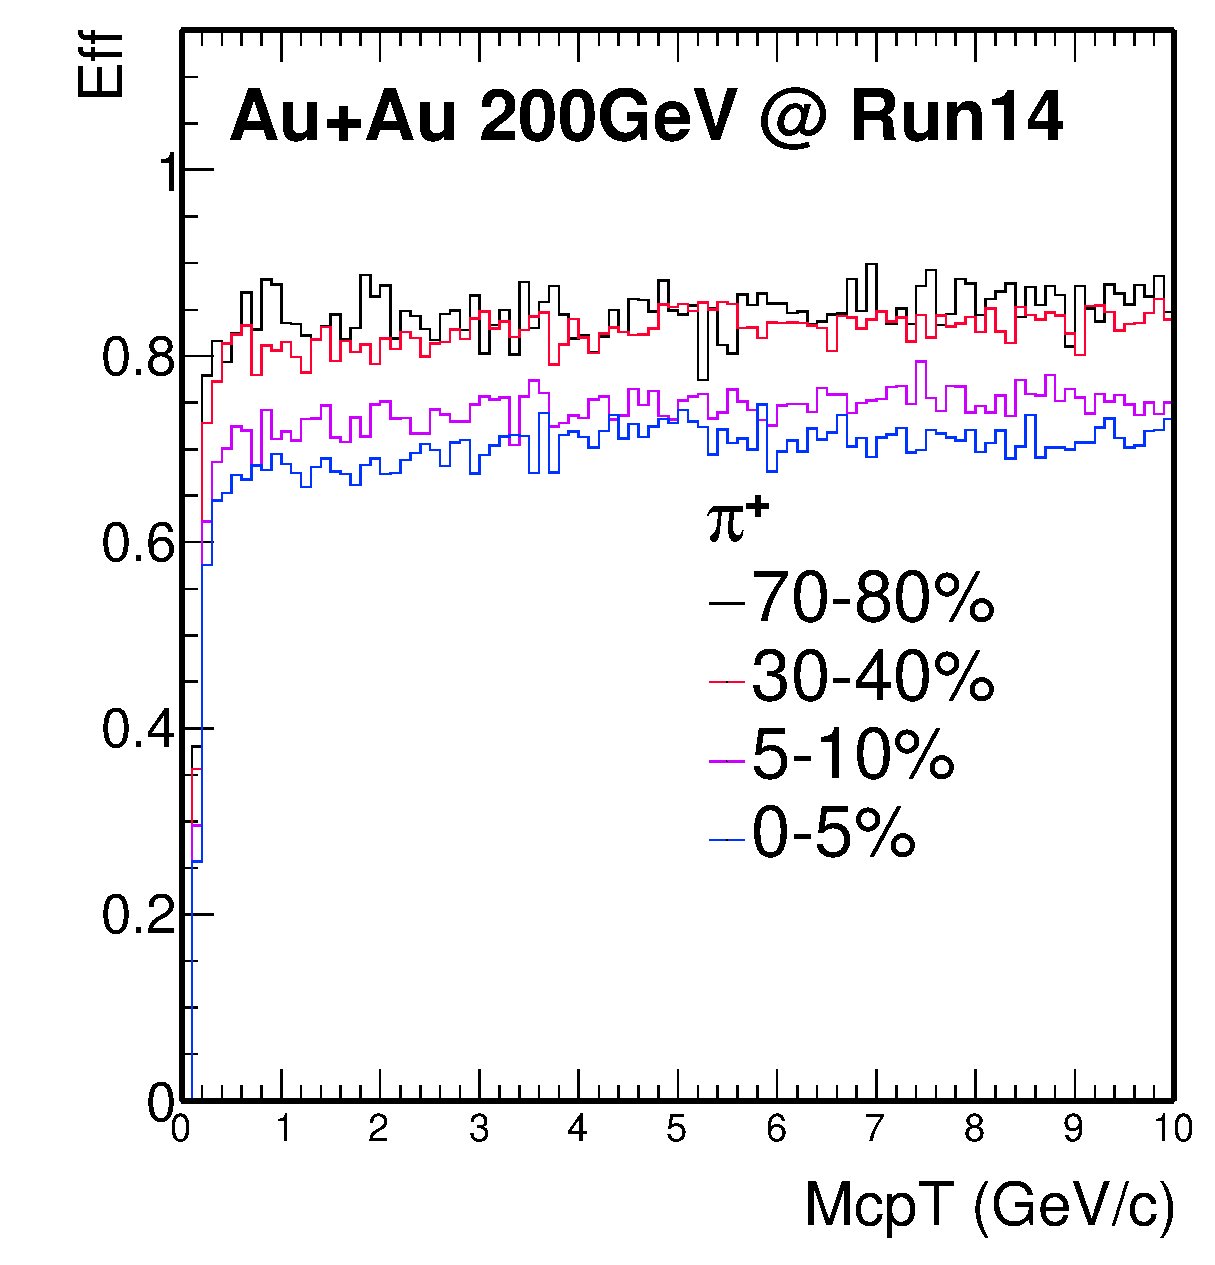
\includegraphics[width=1.0\textwidth]{figure/Run14_D0HFT/pion.eps}
\caption{TPC tracking efficiency in Run14 Au+Au collisions at 200 GeV for Pion. \label{fig:mpion}}
\end{minipage}
\hfill
\begin{minipage}[htbp]{0.52\linewidth}
\centering
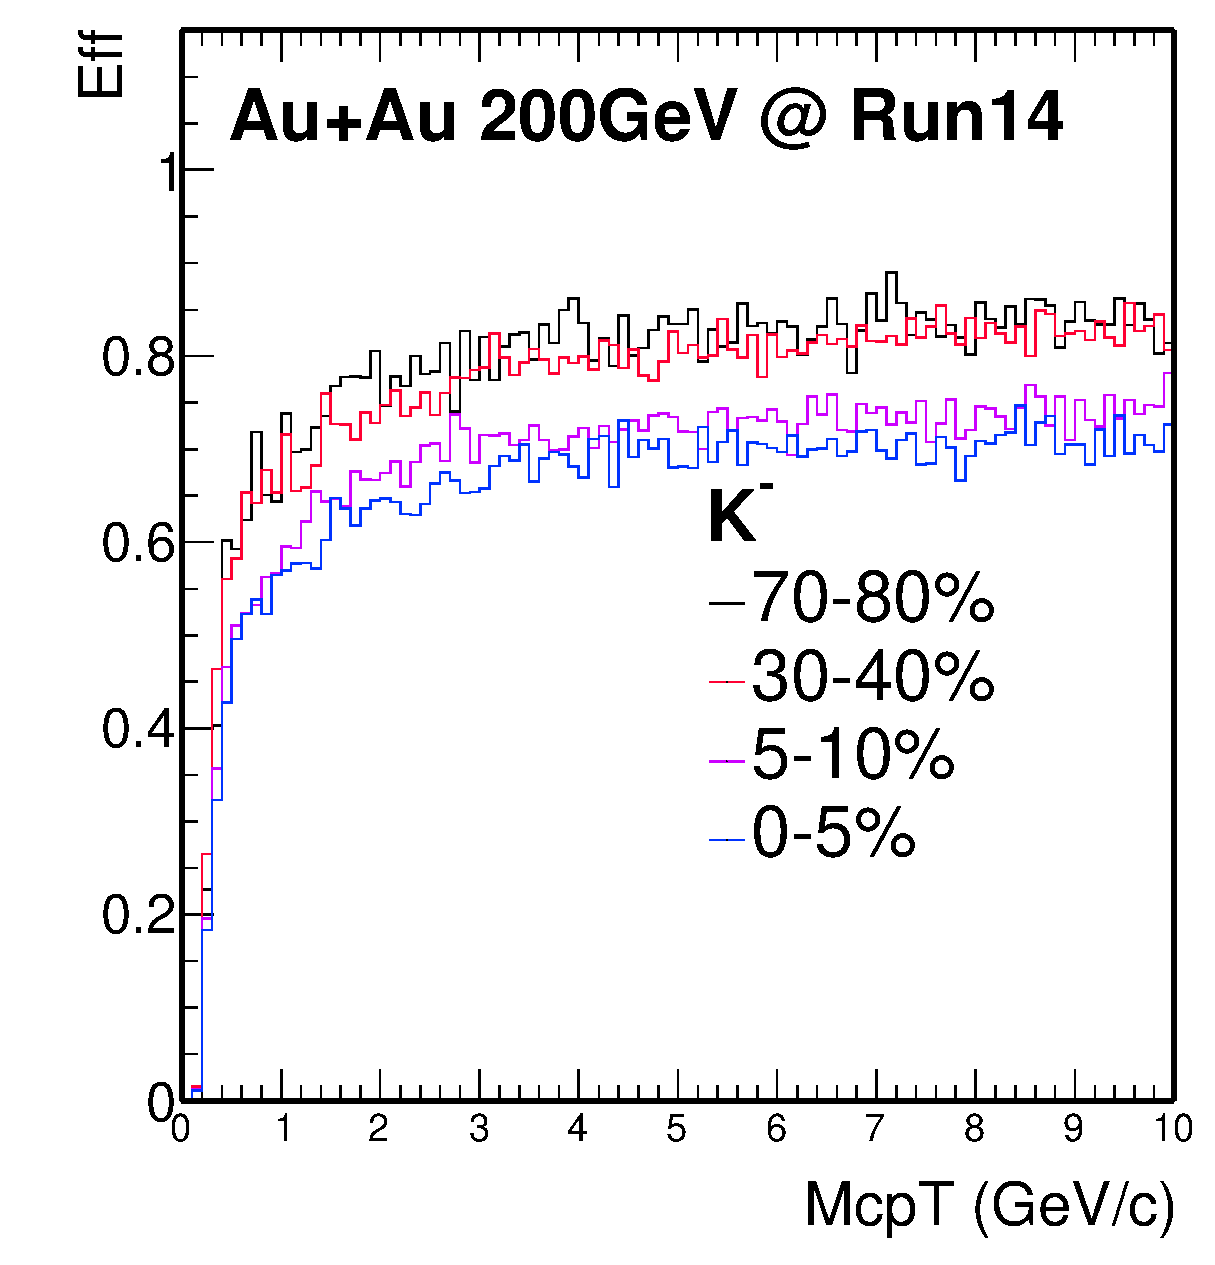
\includegraphics[width=1.0\textwidth]{figure/Run14_D0HFT/kaon.eps} 
\caption{TPC tracking efficiency in Run14 Au+Au collisions at 200 GeV for Kaon. \label{fig:mkaon}}
\end{minipage}
\end{figure}

\subsection{TOF Matching Efficiency \label{sec:TOFmatch}}

For the $D^0$ analysis, we use the hybrid PID for TOF. Which means when TOF is available we use TOF and TPC, when it's not available we just use TPC. The TOF matching efficiency ($\varepsilon_{TOF}$), including the TOF response and the acceptance difference between the TPC and TOF, is evaluated by the real data. It can be calculated by comparing the number of qualified tracks matched with the TOF (with $\beta$ > 0, $N_{matched}$) over  the number of qualified tracks ($N_{TPC}$).

\begin{figure}[htbp]
\begin{minipage}[htbp]{0.52\linewidth}
\centering
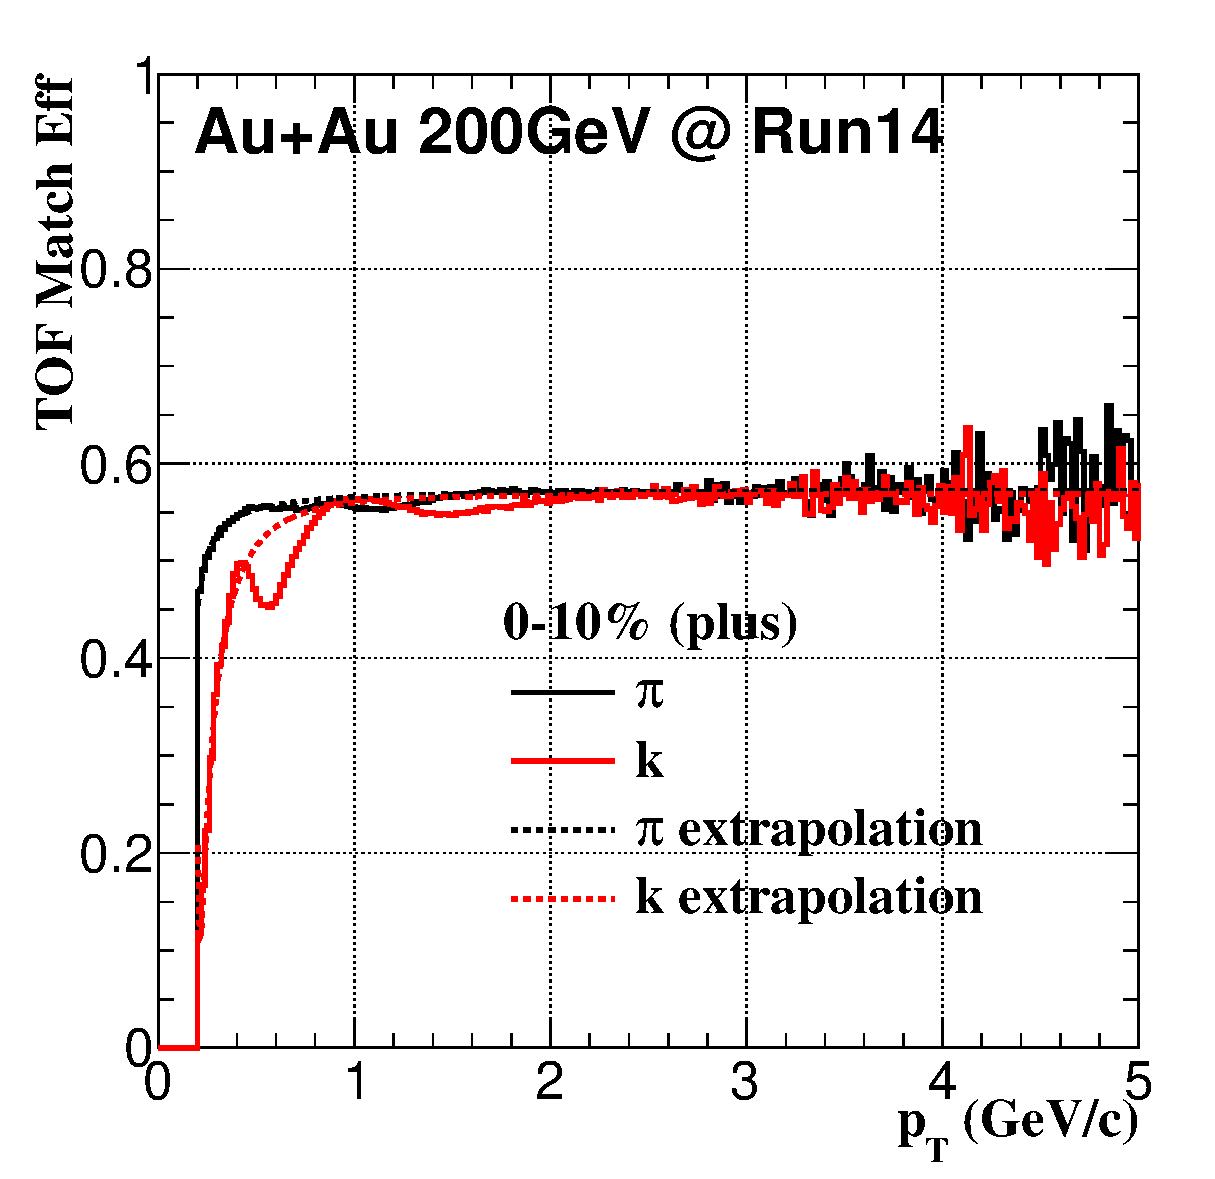
\includegraphics[width=1.0\textwidth]{figure/Run14_D0HFT/tofMatchEff_Run14_Fit_cent1.eps}
\caption{TOF match efficiency in Run14 Au+Au collisions at 200 GeV for positive charge particle in 0-10\%. \label{fig:mtof010}}
\end{minipage}
\hfill
\begin{minipage}[htbp]{0.52\linewidth}
\centering
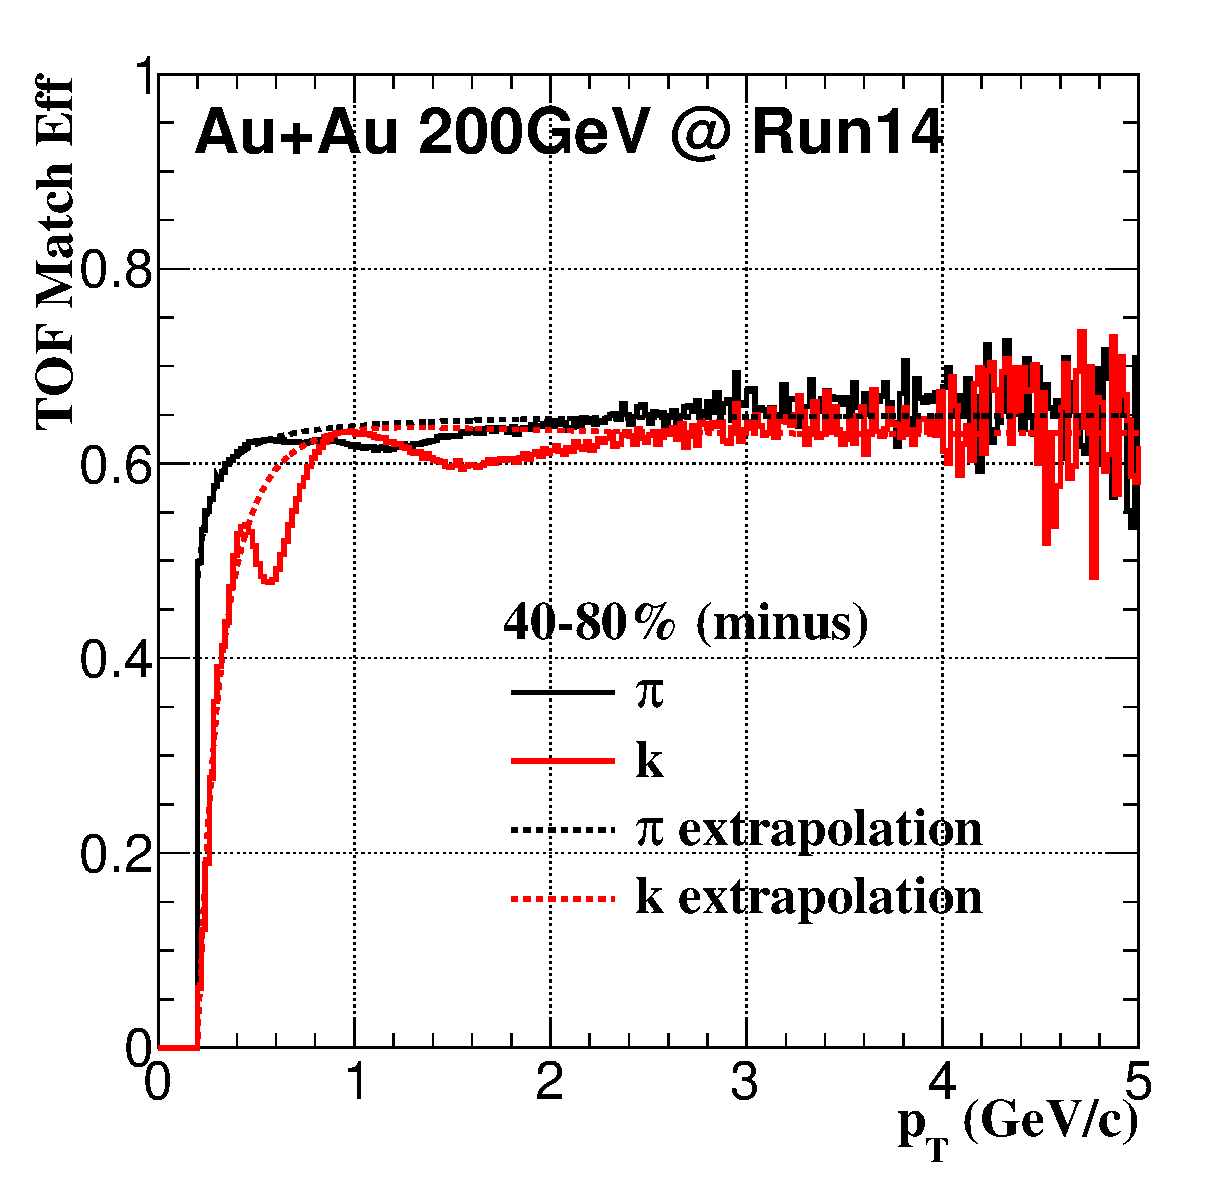
\includegraphics[width=1.0\textwidth]{figure/Run14_D0HFT/tofMatch_minus_Eff_Run14_Fit_cent3.eps} 
\caption{TOF match efficiency in Run14 Au+Au collisions at 200 GeV for negative charge particle in 40-80\%. \label{fig:mtof4080}}
\end{minipage}
\end{figure}


Fig.~\ref{fig:mtof010} shows the TOF match efficiency in Run14 Au+Au collisions at 200 GeV for positive charge particles such as $\pi^{+}$,$K^{+}$ in the centrality 0-10\%. Fig.~\ref{fig:mtof4080} shows the same plots for negative charge particles in the centrality from 40-80\%. For the pion TOF match efficiency, the tread is much smooth compare to kaon. As we see, there are some deep for the TOF match efficiency at some certain $p_{T}$ range from kaon, such as kaon in the $p_{T}$ around 0.6 GeV/$c$. This effect was studied using Hijing simulation, it's found that this is due to the hadron contaminations. 

Fig.~\ref{fig:tpck2} shows the $n\sigma_{K}$ distributions from Hijing in the $p_{T}$ range from 0.5 - 0.7 GeV/$c$. The solid lines are for particles from TPC , and the dashed lines are for particles also include TOF match information. The total yield was scaled to have the same number of pions for this comparison, since the TOF matching have $\sim$30-40\% efficiency lost. In a simple case, if we select kaons with the cut $|n\sigma_{K}| < 1 $, after the requiring of TOF match,the width of this $n\sigma_{K/\pi}$ distribution changed, and the contaminations from pions are reduced. As what we see the dashed black line have less contributions to the kaons peak within $|n\sigma_{K}| < 1$ compare to the solid black line. We also checked this effect in the other $p_{T}$ range such as 0.2 - 0.5 GeV/$c$ and 1.0 - 1.5 GeV/$c$ as shown in Fig.~\ref{fig:tpck1} and Fig.~\ref{fig:tpck3}. This effect is neglectable in the low $p_{T}$ range 0.2 - 0.5 GeV/$c$ since the TPC can well separate pions and kaon. In the high $p_{T}$ range, the dE/dex are overlap with each other for kaon and pion, it's not able to distinguish them only use TPC.

\begin{figure}[htbp]
\centering
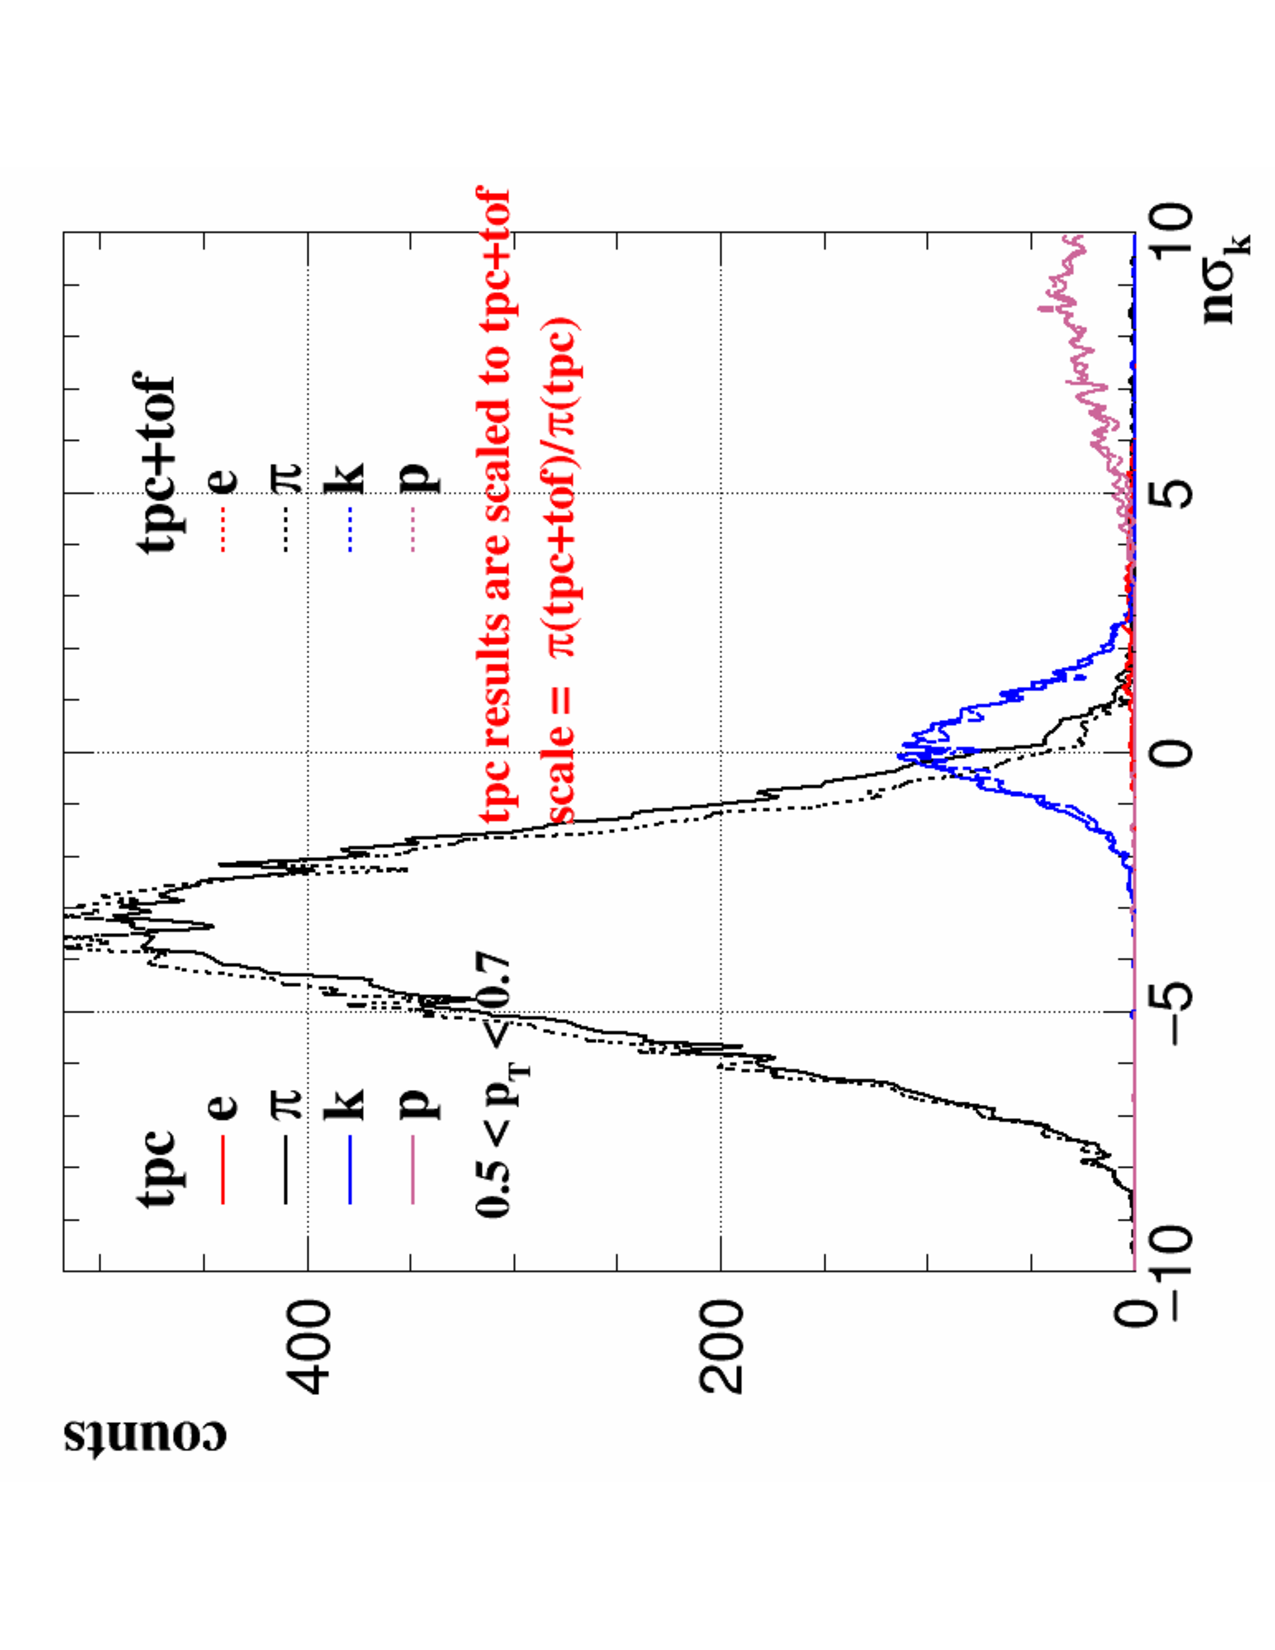
\includegraphics[keepaspectratio,width=0.6\textwidth,angle=-90]{figure/Run14_D0HFT/tofMatch_Hijing_nSigmaK.pdf}
\caption{$n\sigma_{K}$ distributions for 0.5 < $p_T$ < 0.7 GeV/$c$. The solid lines are from TPC and dashed lines are from TPC + TOF.}
\label{fig:tpck2}
\end{figure}

\begin{figure}[htbp]
\begin{minipage}[htbp]{0.52\linewidth}
\centering
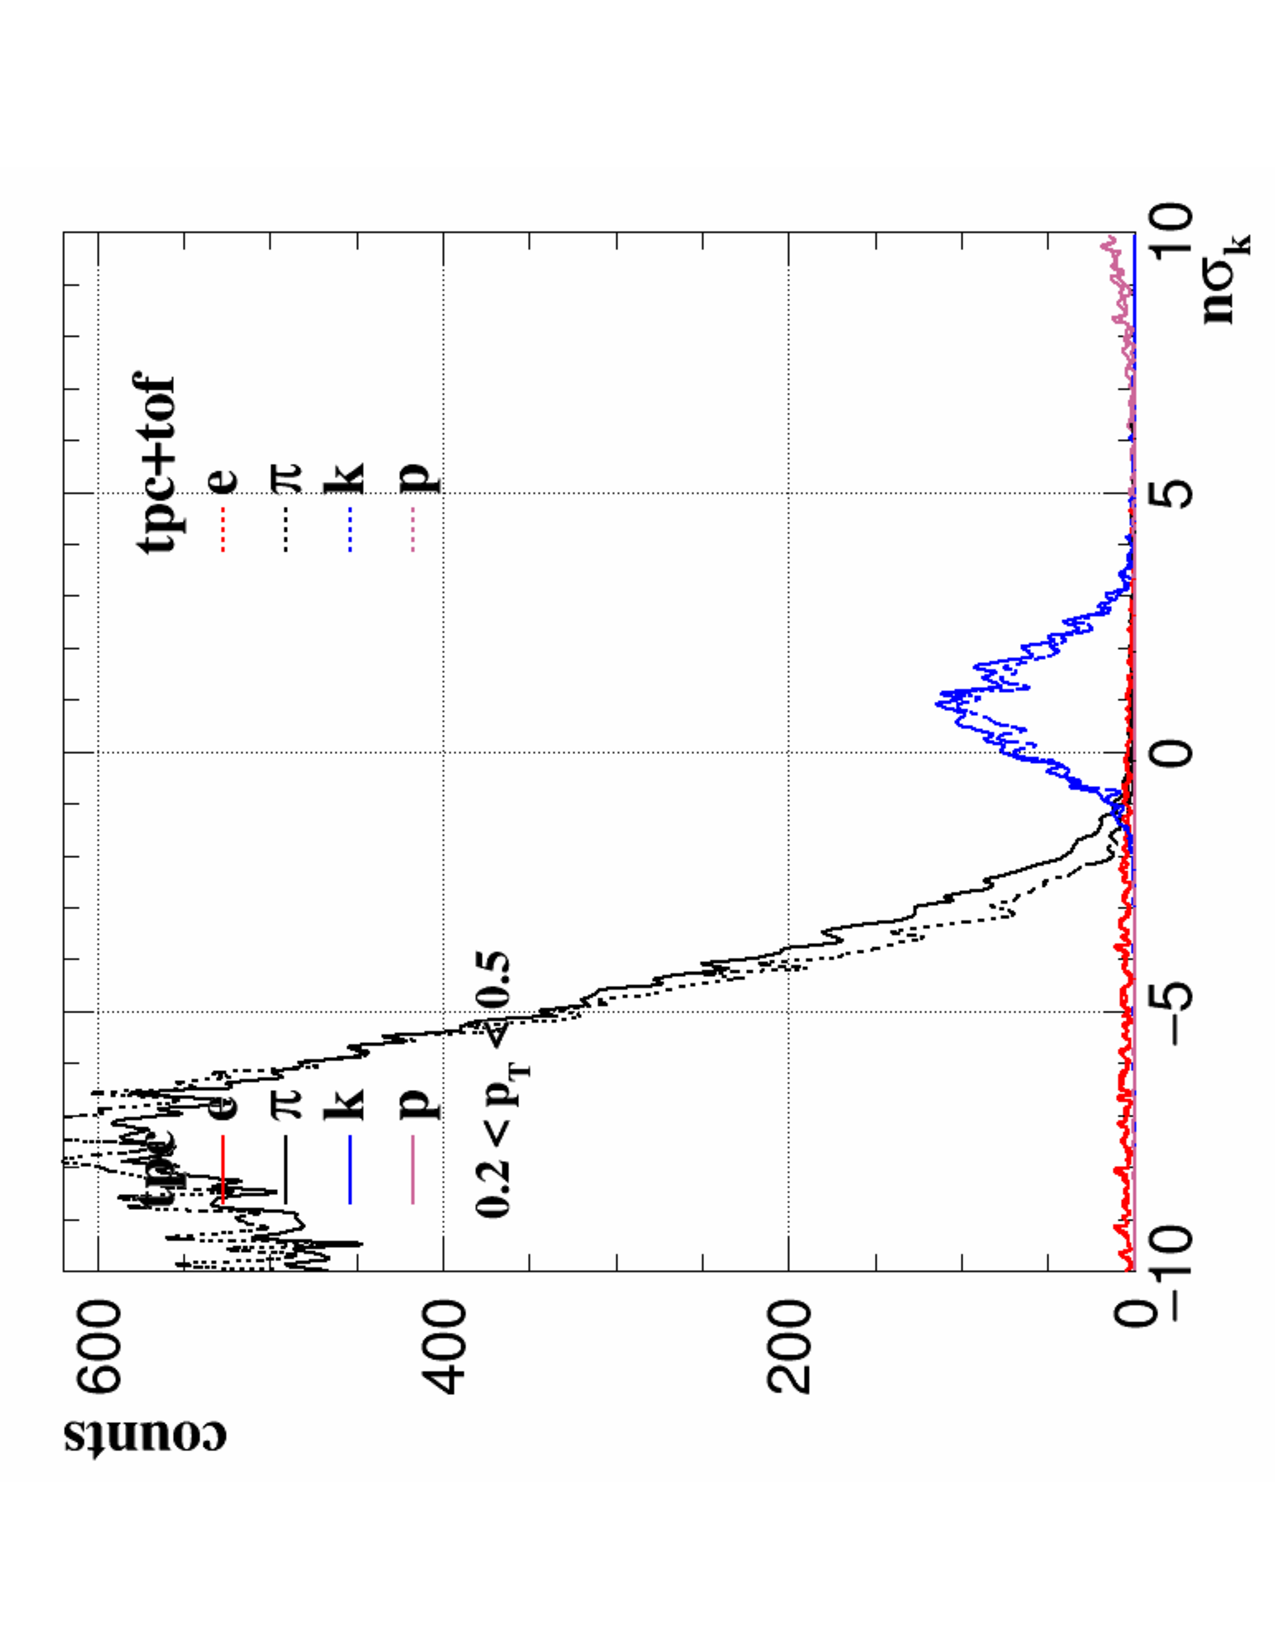
\includegraphics[width=1.0\textwidth,angle=-90]{figure/Run14_D0HFT/tofMatch_Hijing_nSigmaK1.pdf}
\caption{$n\sigma_{K}$ distributions for 0.2 < $p_T$ < 0.5 GeV/$c$. The solid lines are from TPC and dashed lines are from TPC + TOF.\label{fig:tpck1}}
\end{minipage}
\hfill
\begin{minipage}[htbp]{0.52\linewidth}
\centering
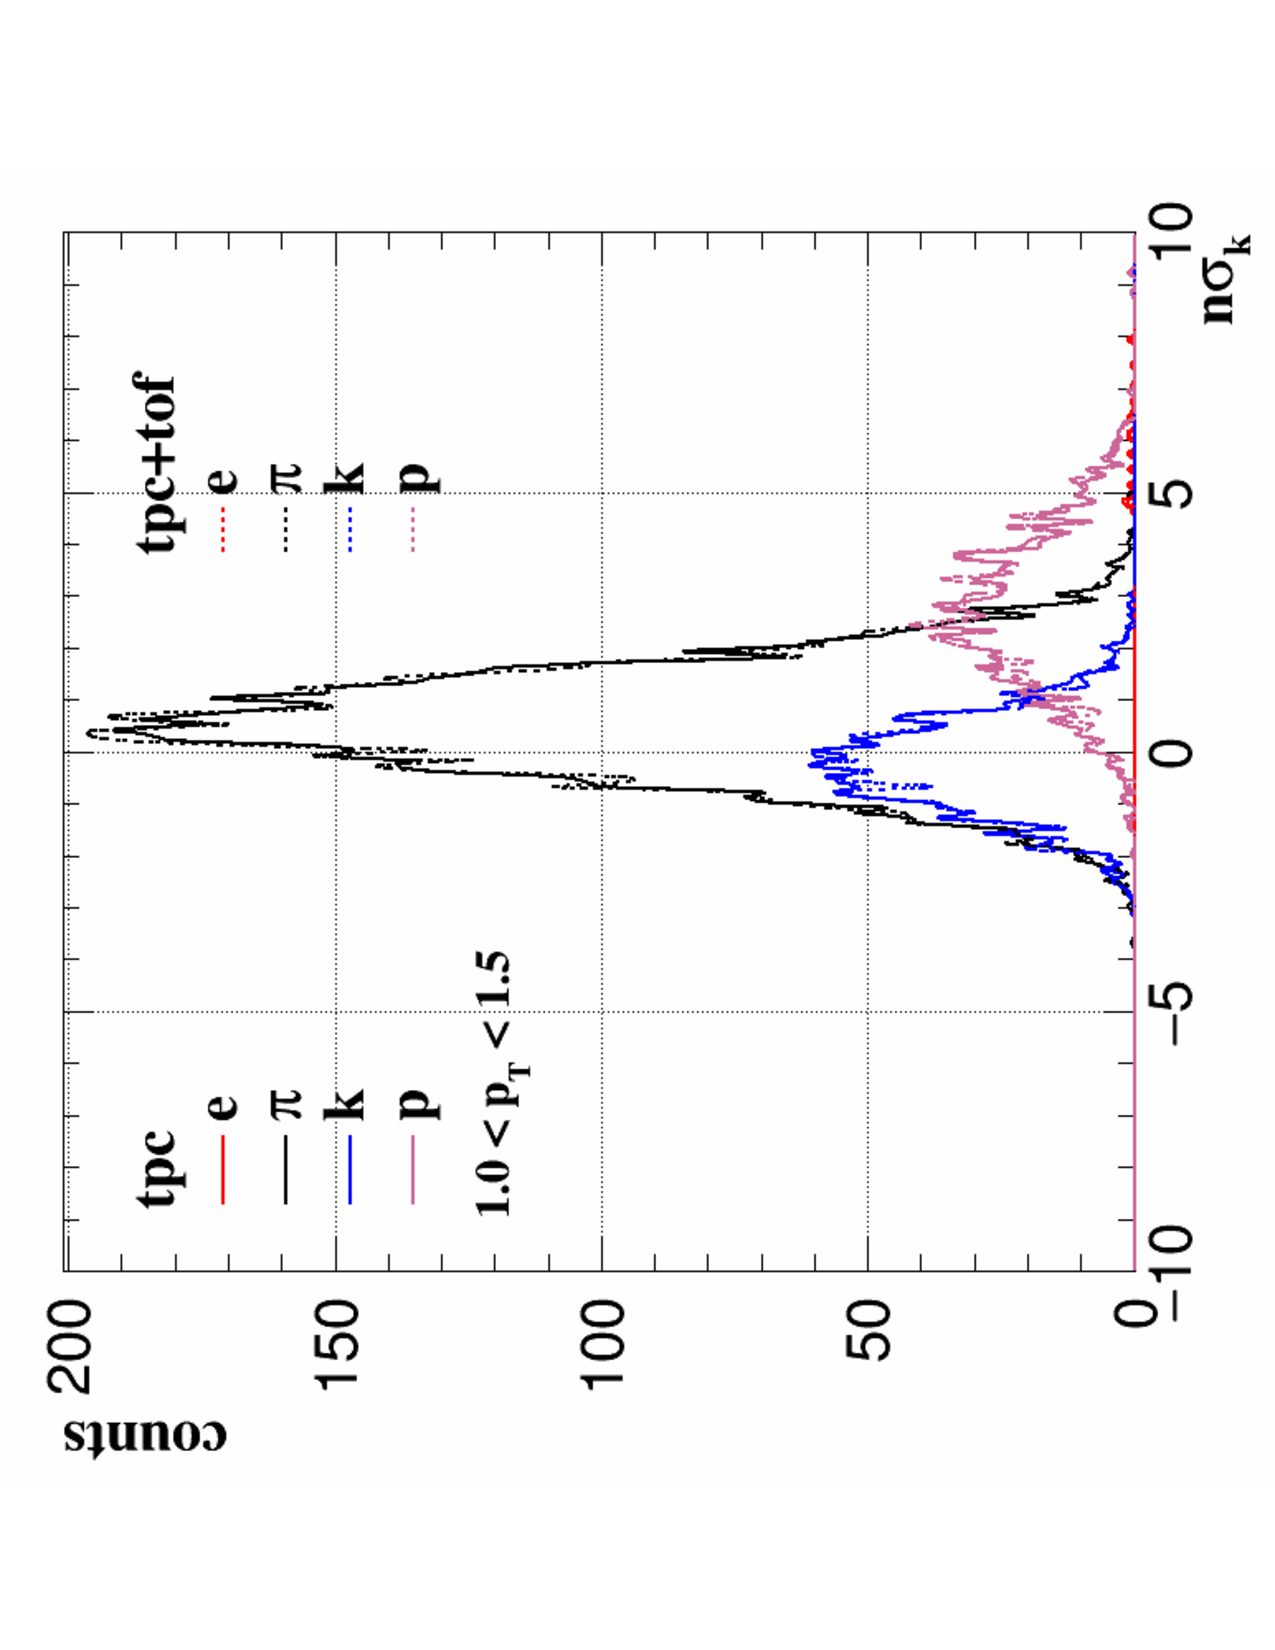
\includegraphics[width=1.0\textwidth,angle=-90]{figure/Run14_D0HFT/tofMatch_Hijing_nSigmaK2.pdf} 
\caption{$n\sigma_{K}$ distributions for 1.0 < $p_T$ < 1.5 GeV/$c$. The solid lines are from TPC and dashed lines are from TPC + TOF.\label{fig:tpck3}}
\end{minipage}
\end{figure}

\subsection{PID Cut Efficiency}
\label{pideff}
The particle identification cut efficiency ($\varepsilon_{PID}$) includes two components: the TOF velocity ($1/\beta$) cut efficiency and $dE/dx$ cut ($n\sigma_{K/\pi}$) efficiency. Pure pions and kaons sample are used to evaluate the TOF velocity cut efficiency and TPC $n\sigma_{K/\pi}$ cut efficiency. Fig.~\ref{fig:ksmass} shows the $\pi\pi$ pairs invariant mass distributions. The black line is the unlikesign foreground, and the red line is background using likesign method. With this $K_{s}^{0}$ candidates, we can statistical extract the pure pion sample for the PID efficiency study. Fig.~\ref{fig:phimass} shows the $KK$ pairs invariant mass distributions. Still with the unlikesign and likesign method, the $\Phi$ meson candidates are reconstructed, and we can statistical extract the pure kaon sample for the PID efficiency study.

\begin{figure}[htbp]
\begin{minipage}[htbp]{0.52\linewidth}
\centering
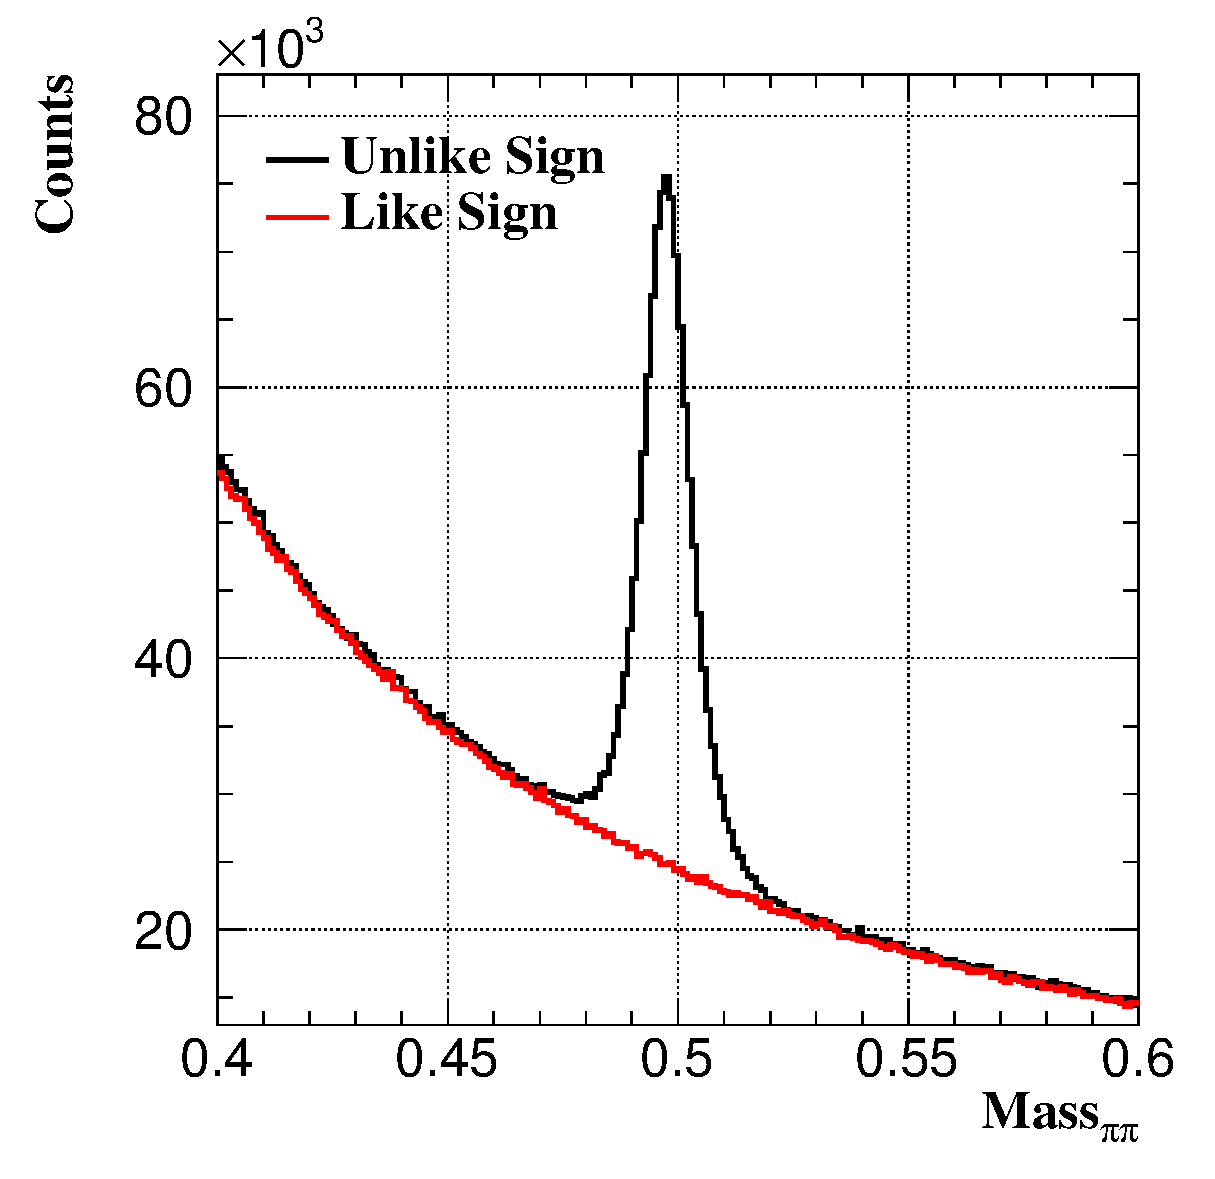
\includegraphics[width=1.0\textwidth]{figure/Run14_D0HFT/massKshort.eps}
\caption{The $\pi\pi$ pairs invariant mass distributions. The black line is the unlikesign foreground, and the red line is background using likesign method. \label{fig:ksmass}}
\end{minipage}
\hfill
\begin{minipage}[htbp]{0.52\linewidth}
\centering
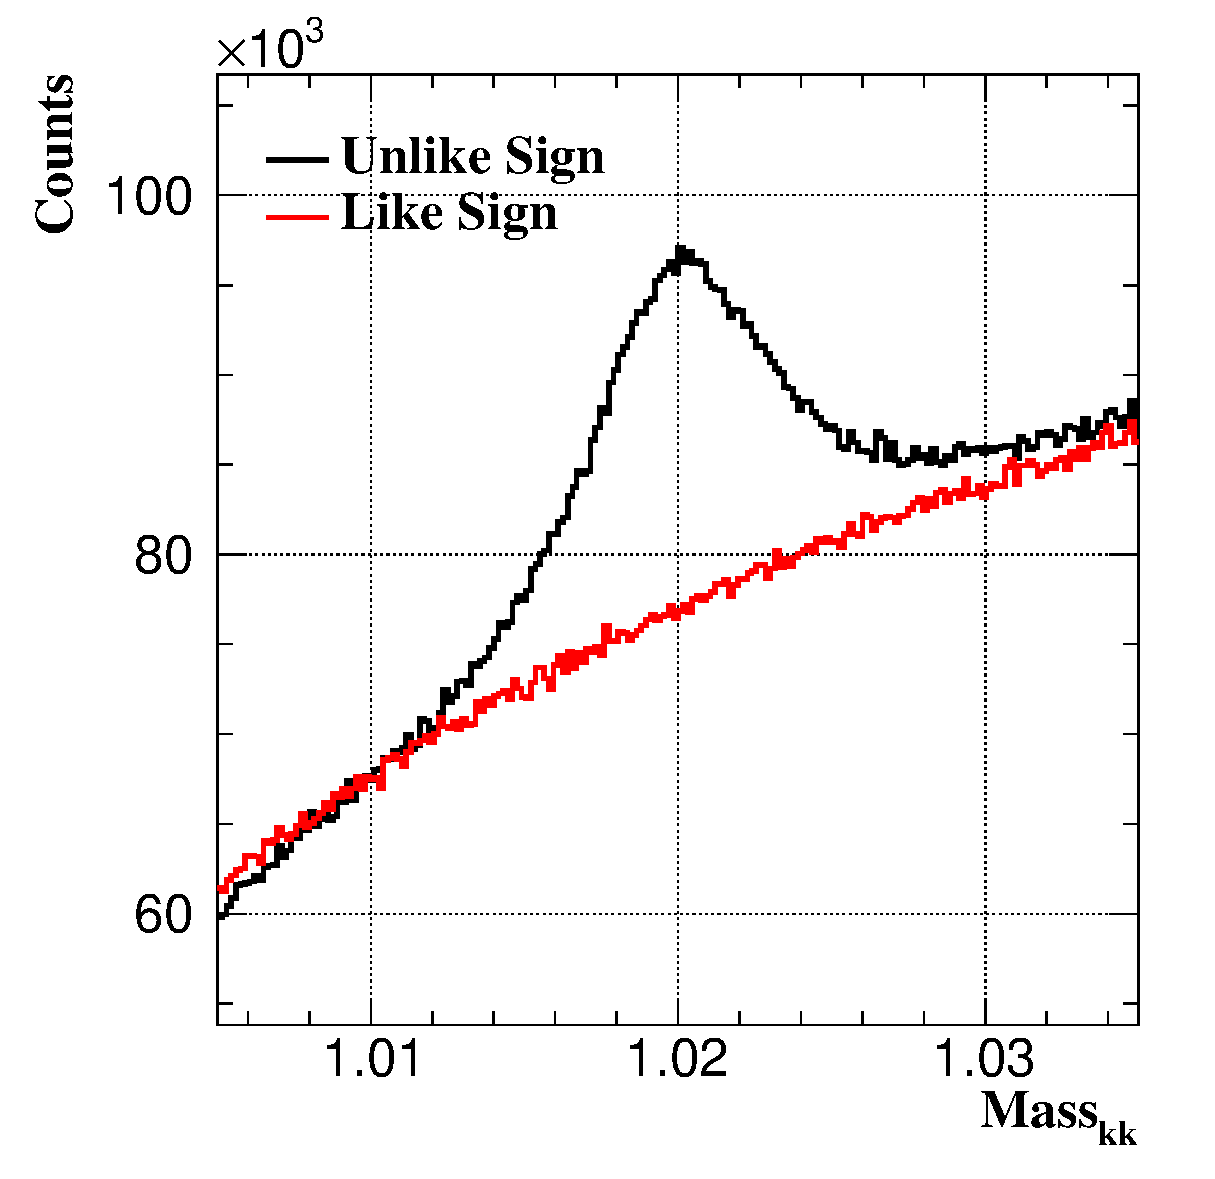
\includegraphics[width=1.0\textwidth]{figure/Run14_D0HFT/massPhi.eps} 
\caption{The $KK$ pairs invariant mass distributions. The black line is the unlikesign foreground, and the red line is background using likesign method. \label{fig:phimass}}
\end{minipage}
\end{figure}

\subsubsection{$n\sigma_{K/\pi}$ Cut Efficiency}

The $n\sigma_{K/\pi}$ cut efficiency is derived from the Gaussian fit using those pure samples. The $n\sigma_{K/\pi}$ distributions are fitted with Gaussian function, the mean value and sigma value are plotted as Fig.~\ref{fig:pionmean} and Fig.~\ref{fig:pionsigma}. With these mean and sigma distributions, assuming they follow the Gaussian function, for example, Fig.~\ref{fig:pionnsigmaeff} depicts the $n\sigma_{\pi}$ cut efficiency in Run14 Au + Au collisions at 200 GeV for pions. For kaons, we use the same method extracting this $n\sigma_{K}$ cut efficiency.

\begin{figure}[htbp]
\begin{minipage}[htbp]{0.5\linewidth}
\centering
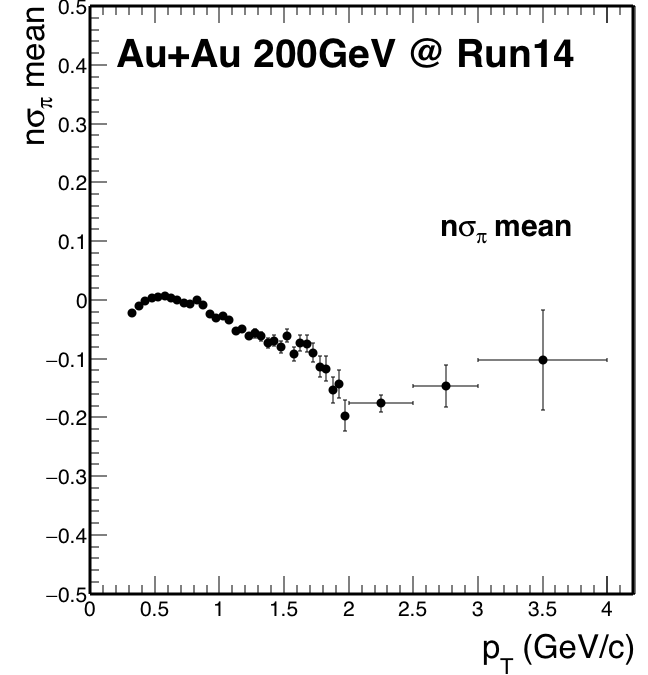
\includegraphics[width=1.0\textwidth]{figure/Run14_D0HFT/nSigPion_mean.png}
\caption{The mean value of $n\sigma_{\pi}$ distributions vs momentum. The red line is fitted function with polynomial function. \label{fig:pionmean}}
\end{minipage}
\hfill
\begin{minipage}[htbp]{0.5\linewidth}
\centering
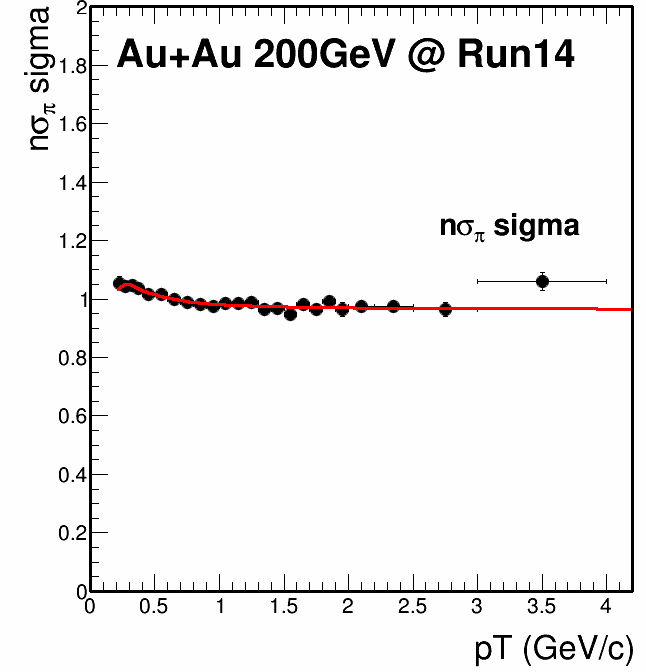
\includegraphics[width=1.0\textwidth]{figure/Run14_D0HFT/nSigPion_sigma.png}
\caption{The sigma value of $n\sigma_{\pi}$ distributions vs momentum. The red line is fitted function with polynomial function. \label{fig:pionsigma}}
\end{minipage}
\end{figure}

\begin{figure}[htbp]
\centering
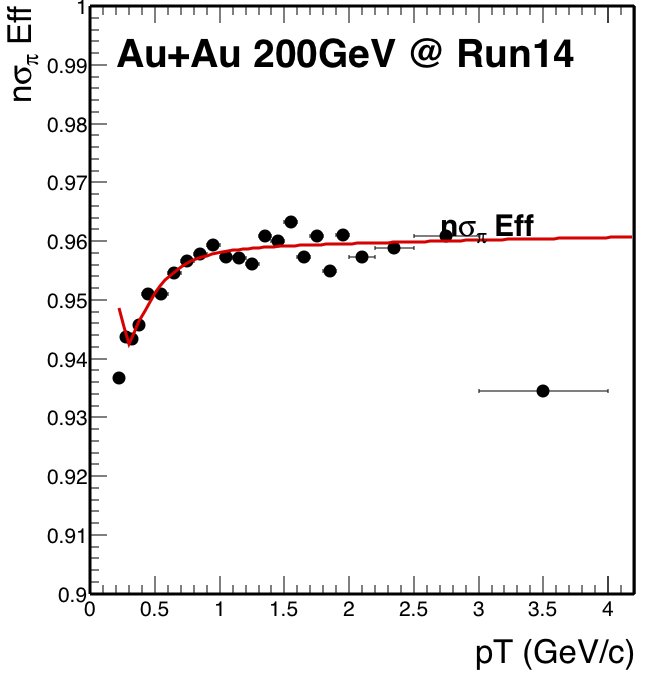
\includegraphics[keepaspectratio,width=0.55\textwidth]{figure/Run14_D0HFT/nSigPion_Eff.png}
\caption{$n\sigma_{\pi}$ cut efficiency along with momentum. Red line is the fitted polynomial function}
\label{fig:pionnsigmaeff}
\end{figure}

\subsubsection{$1/\beta$ Cut Efficiency}
The $1/\beta$ cut efficiency is derived from the 1/$\beta$ distributions, two methods are used, one is the bin counting method and another is using Gaussian fitting and calculate the efficiency from the fitting parameters. The default value is from bin counting and the difference between these two methods are quoted as systematic uncertainties as shown on Fig.~\ref{fig:piontofeff} and Fig.~\ref{fig:kaontofeff} as fitting method. The fluctuations for kaons samples was due to the hadron contaminations at some $p_T$ range. 

\begin{figure}[htbp]
\begin{minipage}[htbp]{0.5\linewidth}
\centering
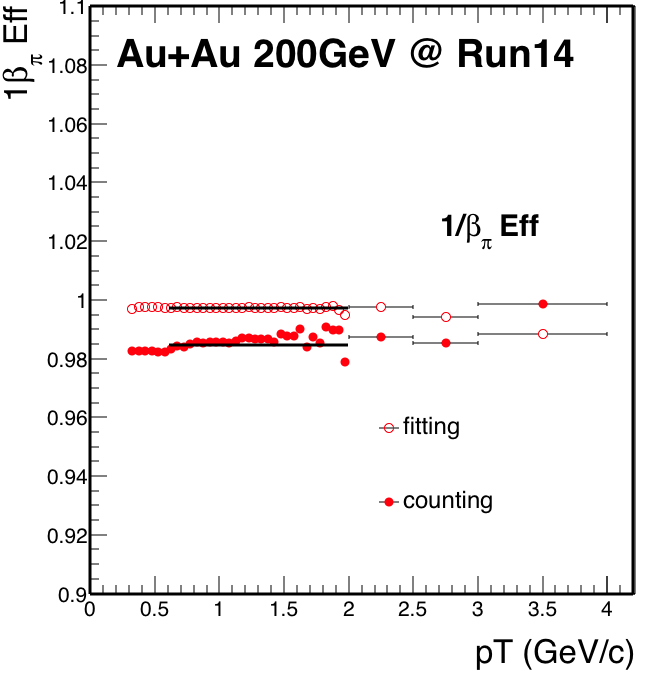
\includegraphics[width=1.0\textwidth]{figure/Run14_D0HFT/nSigPionTof_eff.png}
\caption{$1/\beta$ cut efficiency along with momentum for pion. Red line is the fitted function. \label{fig:piontofeff}}
\end{minipage}
\hfill
\begin{minipage}[htbp]{0.5\linewidth}
\centering
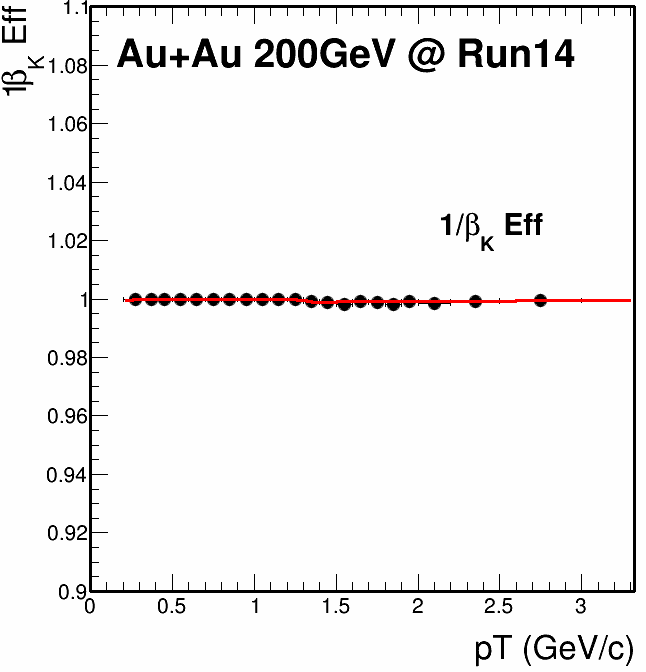
\includegraphics[width=1.0\textwidth]{figure/Run14_D0HFT/nSigKaonTof_eff.png}
\caption{$1/\beta$ cut efficiency along with momentum for kaon. Red line is the fitted function. \label{fig:kaontofeff}}
\end{minipage}
\end{figure}


\subsection{Data-driven fast Monte Carlo setup for HFT and Topological Cut Efficiency}

As discussed in the beginning of this section, the HFT related efficiency shown on Eq.~\ref{effEqu} including two items: HFT acceptance and topological cuts. Since the HFT embedding is not ready yet at that time, we developed the `Data-Driven Fast simulation' for the HFT related efficiency correction. And this method was validated with full GEANT simulation and will be discuss later.

\subsubsection{Assumptions}
\label{assumptions}
Before we discuss the details procedure of the method, it's better to make it clear, this data-driven simulation is based on several assumptions. And the validating will be tested step by step in the later section.
\begin{itemize}
\item Factorization of tracking efficiency:
\begin{equation}
\frac{\textup{HFT}}{\textup{MC}} = \frac{\textup{HFT}}{\textup{TPC}} \times \frac{\textup{TPC}}{\textup{MC}}
\label{efffact}
\end{equation}
\item Spatial resolution of HFT is encoded in two variables: $\textup{DCA}_{\textup{XY}}$ and $\textup{DCA}_{\textup{Z}}$ (two dimensions correlated).
\item Vertex resolution, which is possibly folded in the DCA resolution of single tracks and correlated for kaons and pions, is a negligible, at least for semi-central to central events.
\item The contribution of feed-down particles from secondary decays to DCA distributions is negligible.
\item Mis-matched daughter tracks are removed by topological cuts.
\end{itemize}

\subsubsection{Ingredients}
\label{ingredients}
There are several input ingredients for this fast-simulation package which is extracted from data.
\begin{itemize}
\item Extract $\textup{V}_\textup{z}$ distributions from data (centrality dependent).
\item Extract ratio of HFT matched tracks to TPC tracks from data (This ratio includes all mismatched tracks) (particle species, centrality, $p_T$, $\eta$, $\phi$, $\textup{V}_\textup{z}$ dependence).
\item Extract $\textup{DCA}_{\textup{XY}}$ - $\textup{DCA}_{\textup{Z}}$ distributions from data. Assuming that data DCA distributions is dominated by primary particles (particle species, centrality, $p_T$, $\eta$, $\textup{V}_\textup{z}$ dependence).
\item Extract TPC efficiency and momentum resolution from embedding (particles, centrality and $p_T$ dependence).
\end{itemize}

Fig.~\ref{hftRatioExample} shows an example of the input HFT match ratio in the certain $\eta$, $\textup{V}_\textup{Z}$, $\phi$ and centrality range. The HFT match ratio increase in the low pt range due to the high mismatch occupancy and keep flat in the high $p_T$ range. This ratio have a strong dependence on these differential such as $\eta$ and $\textup{V}_\textup{Z}$ since this is effected by HFT acceptance. Fig.~\ref{DcaExample} shows an example of the $\textup{Dca}_{\textup{XY}}$ vs $\textup{Dca}_{\textup{Z}}$ distribution in the certain $p_T$, $\eta$, $\textup{V}_\textup{Z}$ and centrality range. The axis binning is dynamic binning (non-uniform) since the most central (around 0) part is the dominate part. Limited by the computing memory, the most central part use fine binning and others use the unrefined binning as shown on the plots.

In total, there are 11 ($\phi$) $\times$ 10 ($\eta$) $\times$ 6 ($\textup{V}_\textup{z}$) $\times$ 9 (centrality) $\times$ 2 (particles) 1D histograms (36 $p_T$ binning) for HFT match efficiency.
There are 5 ($\eta$) $\times$ 4 ($\textup{V}_\textup{z}$) $\times$ 9 (centrality) $\times$ 2 (particles) histograms $\times$ 19 ($p_T$) 2D histograms (144 $\times$ 144 Dca binning) for Dca resolution smearing.

Effectively, these 1D and 2D histograms encode HFT efficiency, acceptance and spatial resolution performance in Run14 data.

\begin{figure}[htbp]
\begin{minipage}[htbp]{0.52\linewidth}
\centering
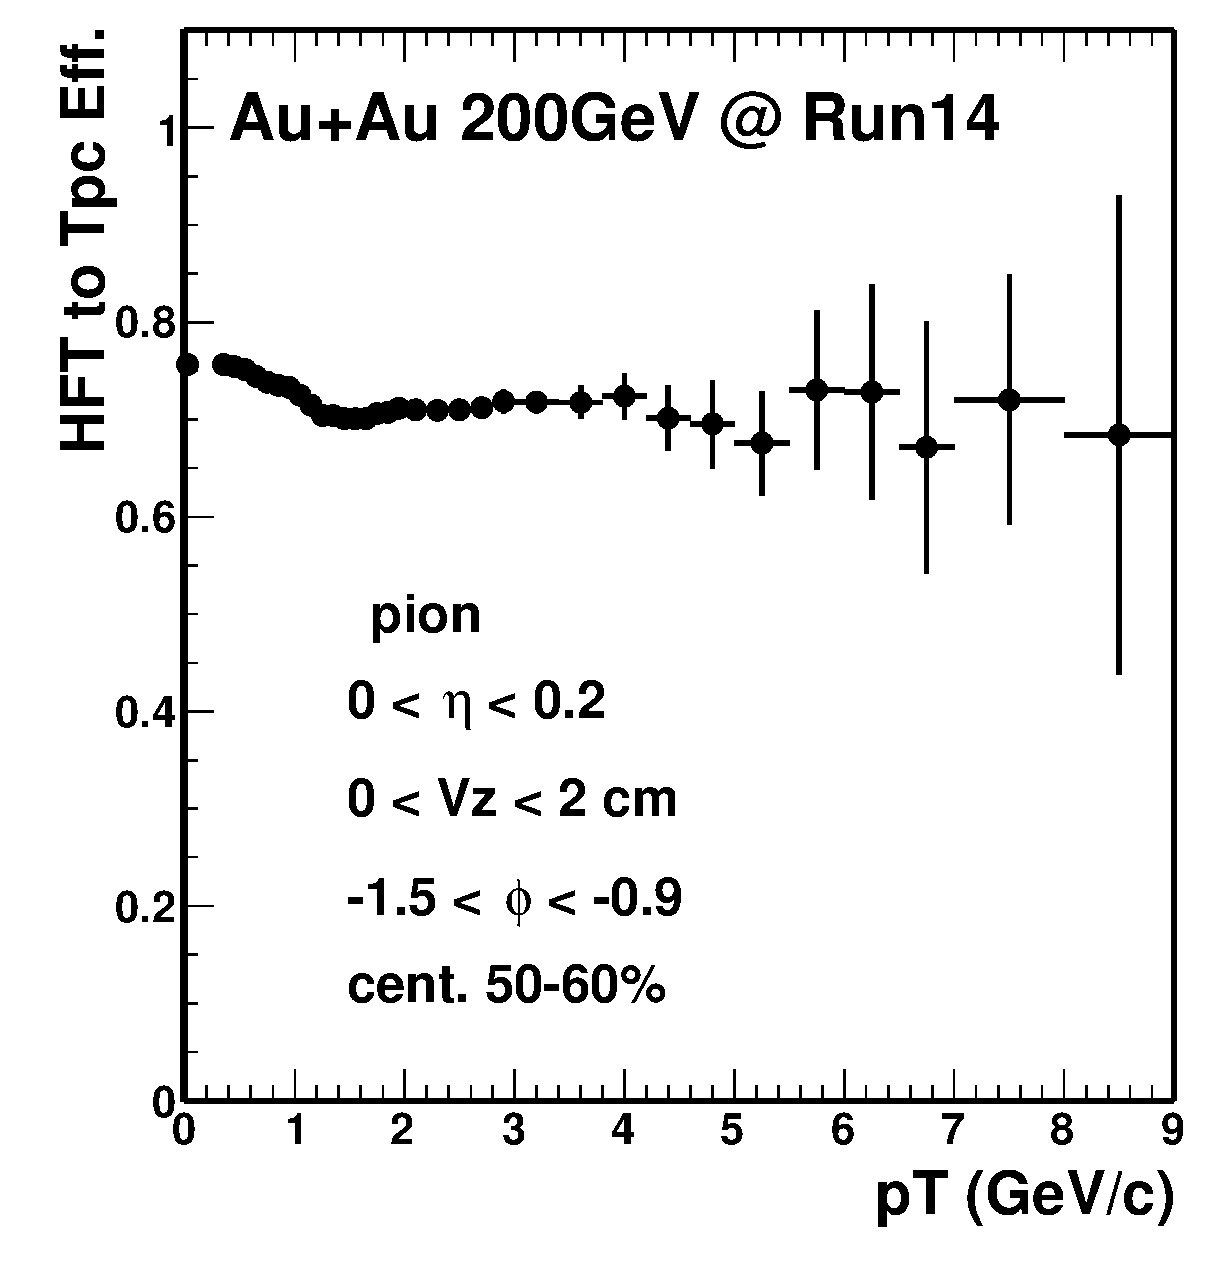
\includegraphics[width=1.0\textwidth,angle=0]{figure/Run14_D0HFT/hftRatioExample.eps}
\caption{ HFT to TPC track match ratio for pion at certain $\eta$,$\textup{V}_{\textup{Z}}$,$\phi$,centrality range. \label{hftRatioExample}}
\end{minipage}
\hfill
\begin{minipage}[htbp]{0.52\linewidth}
\centering
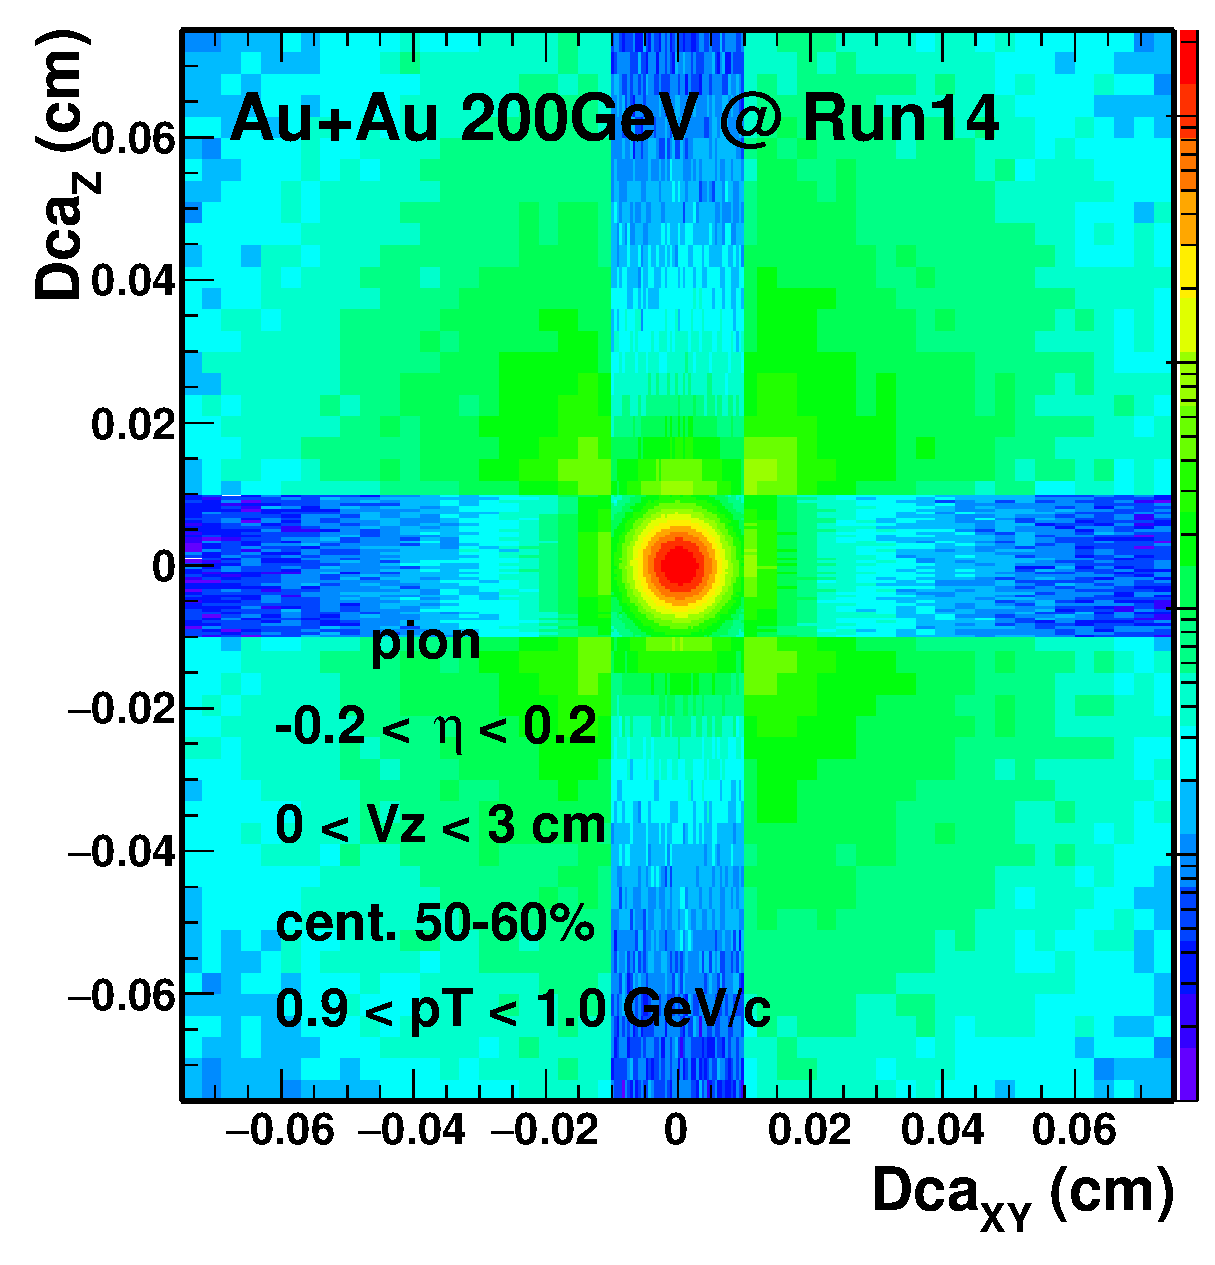
\includegraphics[width=1.0\textwidth,angle=0]{figure/Run14_D0HFT/DcaExample.eps} 
\caption{$\textup{Dca}_{\textup{XY}}$ vs. $\textup{Dca}_\textup{Z}$ for pion at certain $\eta$,$\textup{V}_{\textup{Z}}$,centrality range. \label{DcaExample}}
\end{minipage}
\end{figure}

\subsubsection{Recipe}
\label{recipe}
After all the input ingredients ready for the fast-simulation, a simple toy MC simulation (PYTHIA/EvtGen) is applied for the efficiency study. The basic recipe is following:
\begin{itemize}
\item Sample $\textup{V}_\textup{z}$ distribution according to data distribution.
\item Generate $D^0$ flat in $p_T$ and rapidity and decay it.
\item Smear momentum according the embedding.
\item Smear $DCA_{\textup{XY}}$ and $DCA_\textup{Z}$ of Kaons and Pions independently according to distributions from data.
\item Apply HFT matching efficiency from HFT ratio.
\item Apply TPC reconstruction efficiency.
\item Reconstruct $D^0$
\end{itemize}

\subsubsection{$D^0$ Efficiency and Topological Distribution}

As discussed in the recipe, we obtain the efficiency step by step as shown on Fig.~\ref{D0effStep1} to Fig.~\ref{D0effStep3}.  First we have the TPC efficiency shown by red maker which is after the $p_T$, $\eta$ acceptance cut and TPC tracking efficiency from embedding. Then after folding in the HFT matching efficiency, the second item is obtained on black circle. Last step is after the topological cut, as shown by the cyan marker. As see in the low $p_T$ part, the topological cut efficiency is really small due to the tight cut as the combinatorial background is huge.

% \begin{figure}[htbp]
% \begin{minipage}[htbp]{0.52\linewidth}
% \centering
% 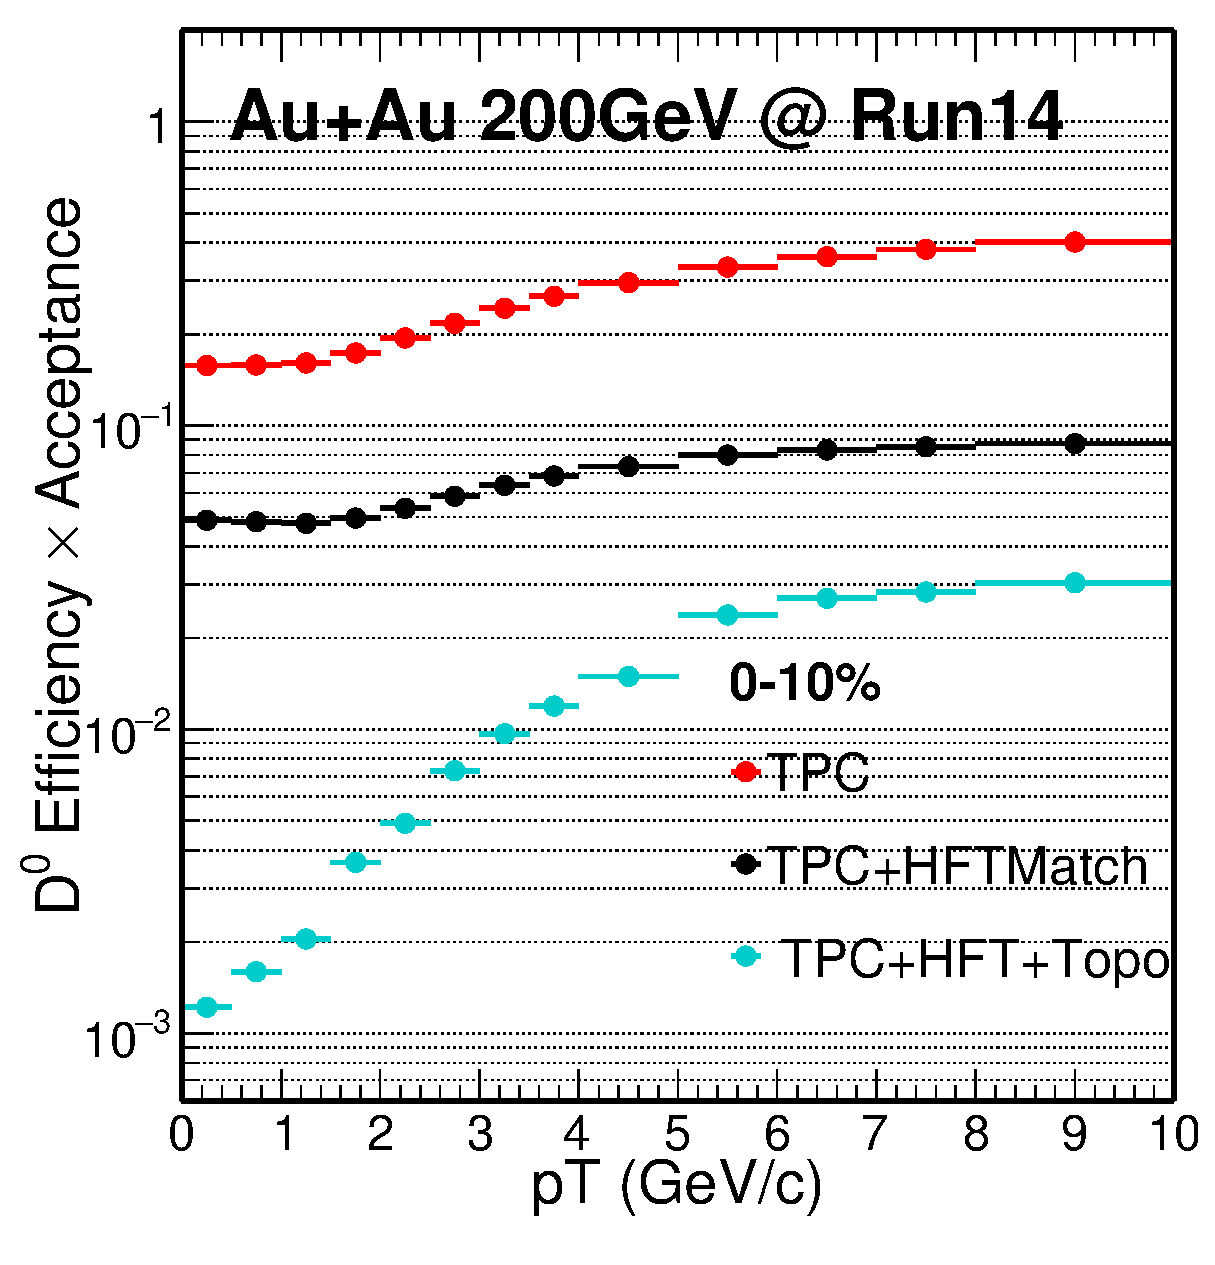
\includegraphics[width=1.0\textwidth,angle=0]{figure/Run14_D0HFT/HFT_efficiencyCombineStepbyStep_2.eps}
% \caption{ $D^0$ efficiency step by step from TPC, HFT Ratio, Topological cut in most central 0-10\%. \label{D0effStep}}
% \end{minipage}
% \hfill
% \begin{minipage}[htbp]{0.52\linewidth}
% \centering
% 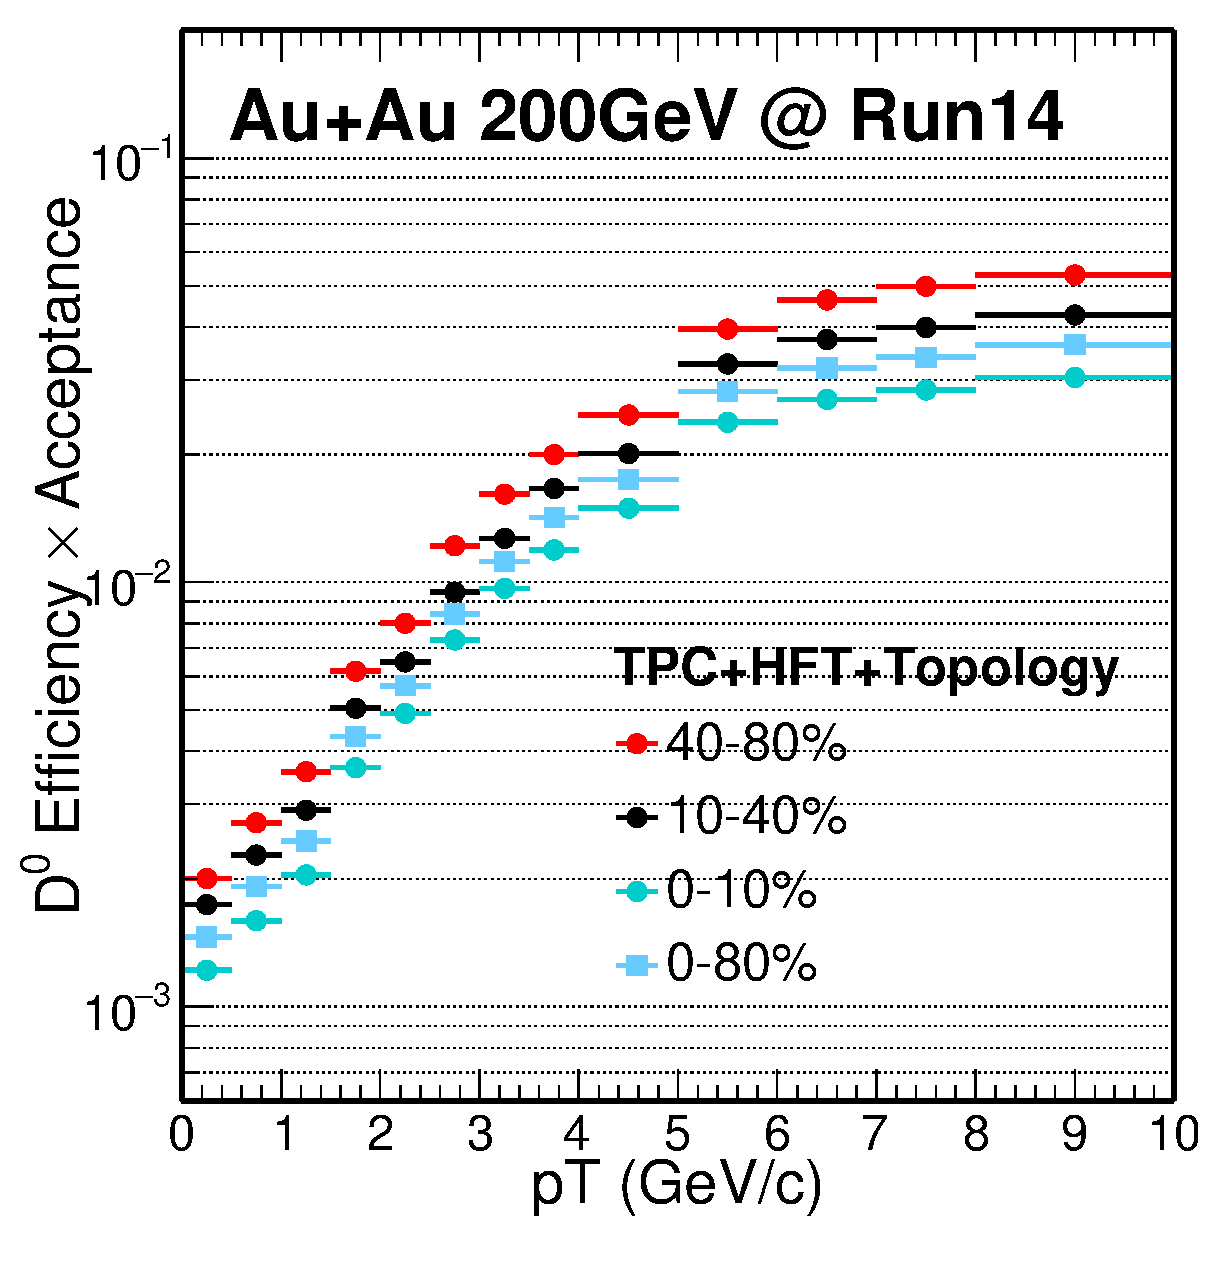
\includegraphics[width=1.0\textwidth,angle=0]{figure/Run14_D0HFT/HFT_efficiencyCombineCompare_5.eps} 
% \caption{ $D^0$ efficiency including TPC, HFT and Topological cut in several centralities. \label{D0effCombine}}
% \end{minipage}
% \end{figure}

\begin{figure}[htbp]
\begin{minipage}[htbp]{0.52\linewidth}
\centering
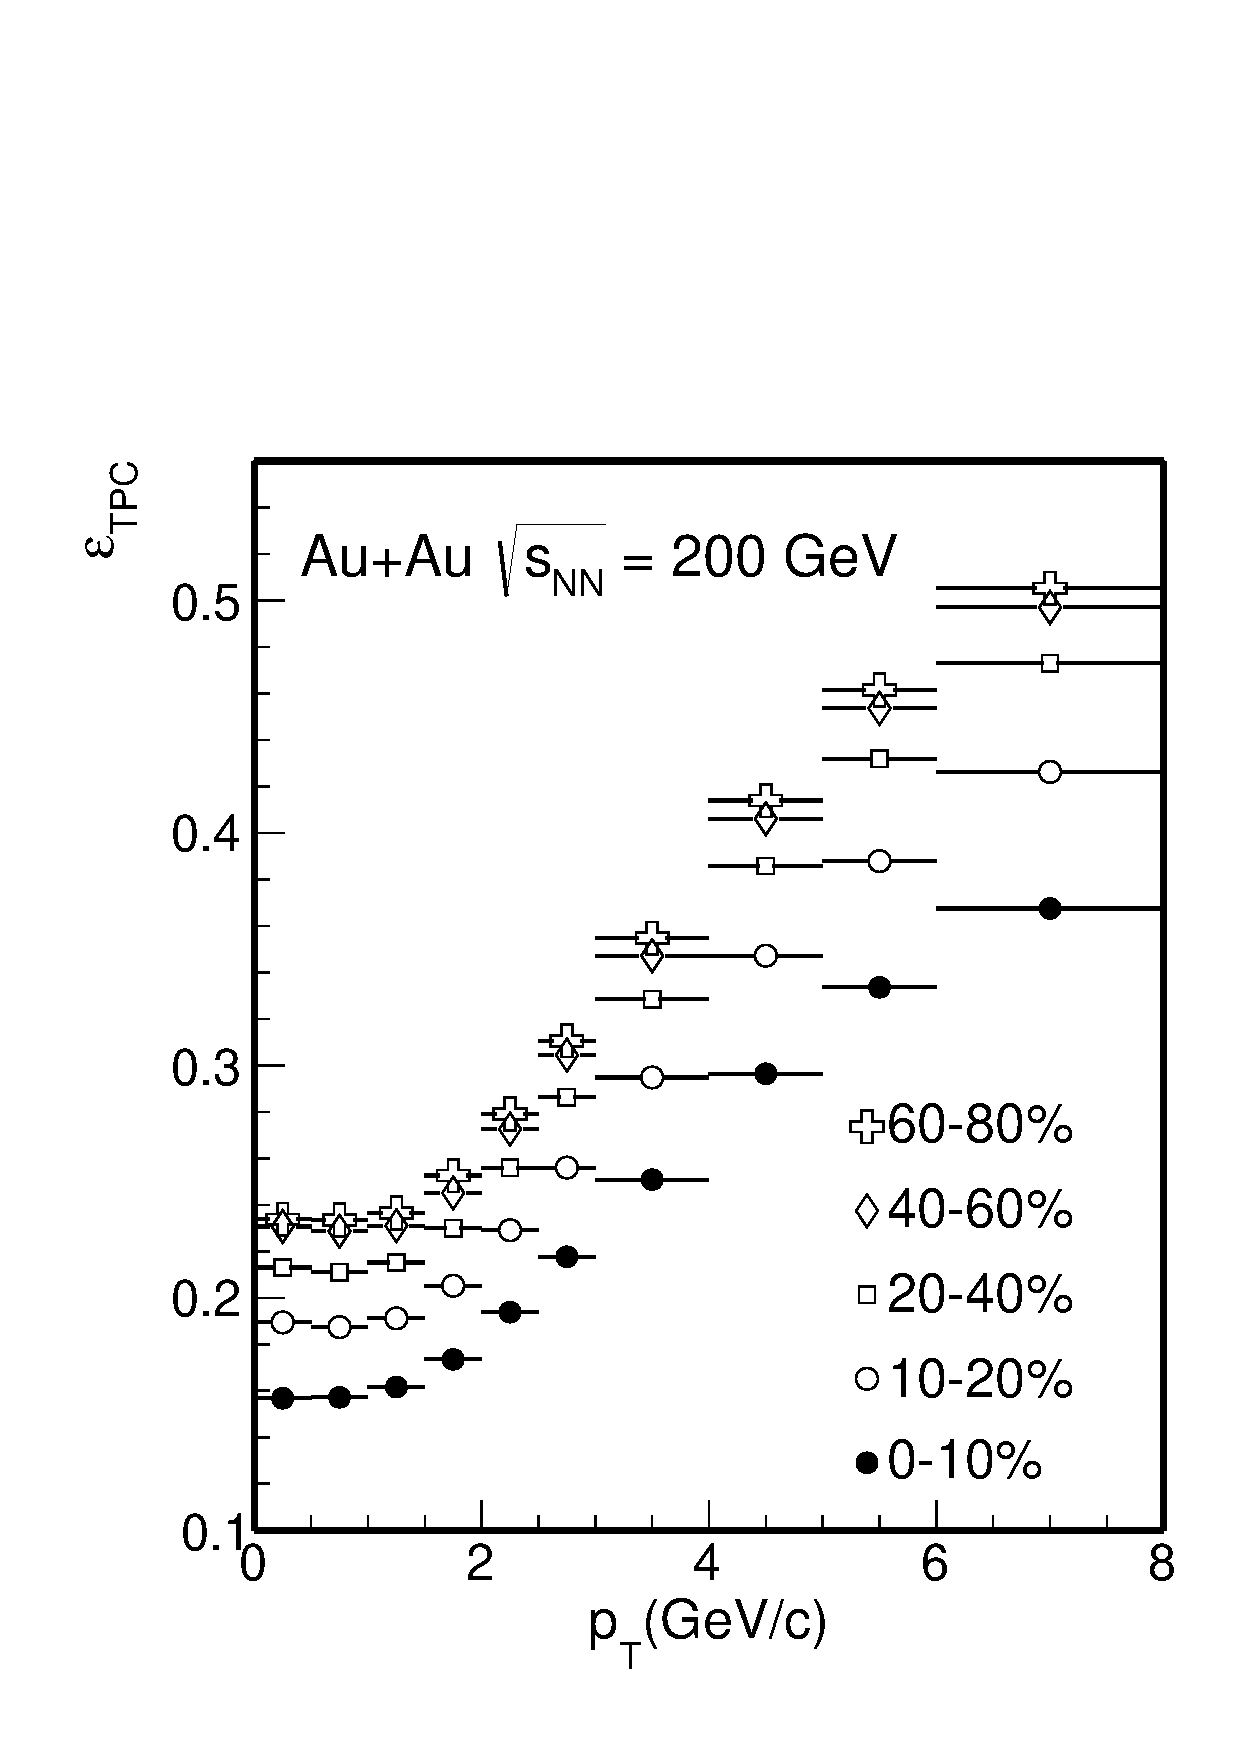
\includegraphics[width=1.0\textwidth,angle=0]{figure/Run14_D0HFT/Datad0Eff_tpc.pdf}
\caption{ $D^0$ efficiency step by step from TPC in different centralities. \label{D0effStep1}}
\end{minipage}
\hfill
\begin{minipage}[htbp]{0.52\linewidth}
\centering
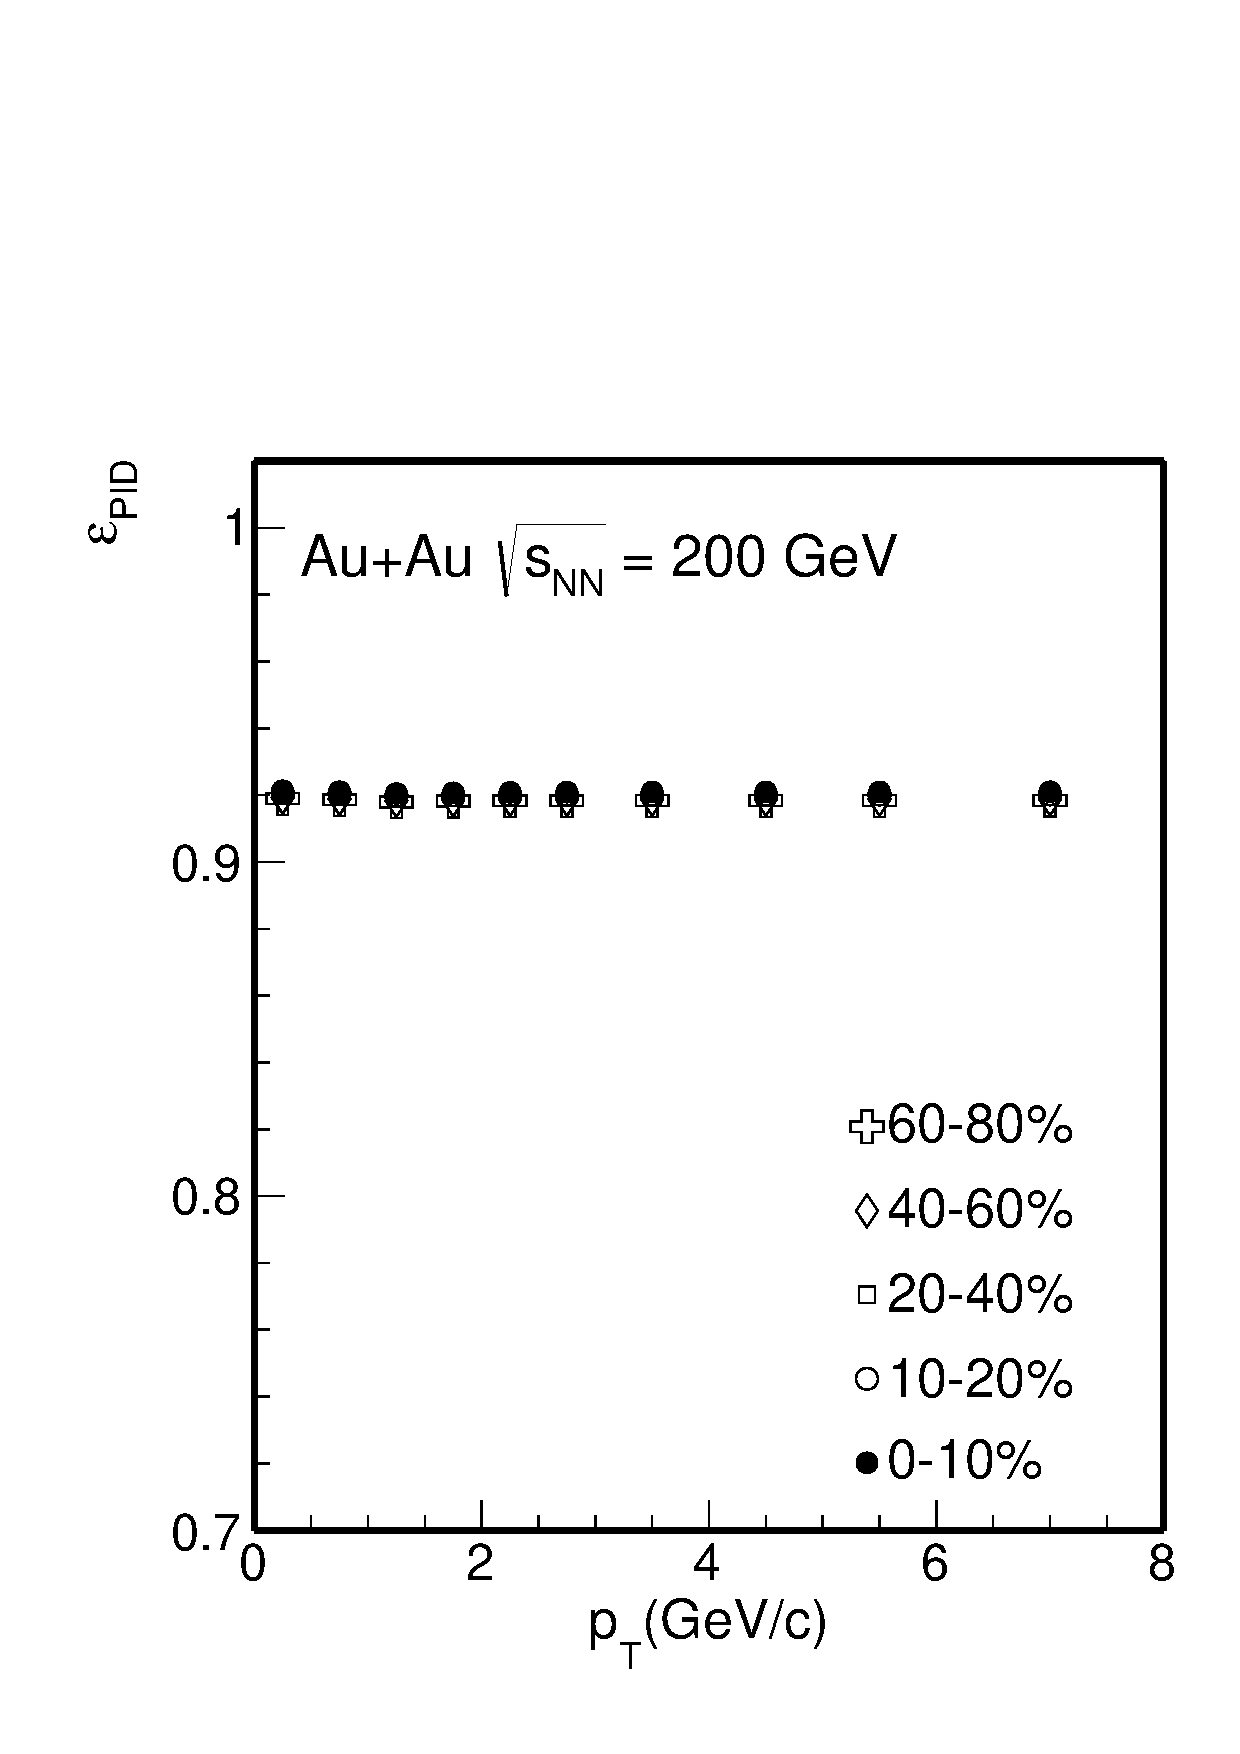
\includegraphics[width=1.0\textwidth,angle=0]{figure/Run14_D0HFT/Datad0Eff_pid.pdf} 
\caption{ $D^0$ efficiency including PID in several centralities. \label{D0effStep2}}
\end{minipage}
\end{figure}

\begin{figure}[htbp]
\begin{minipage}[htbp]{0.52\linewidth}
\centering
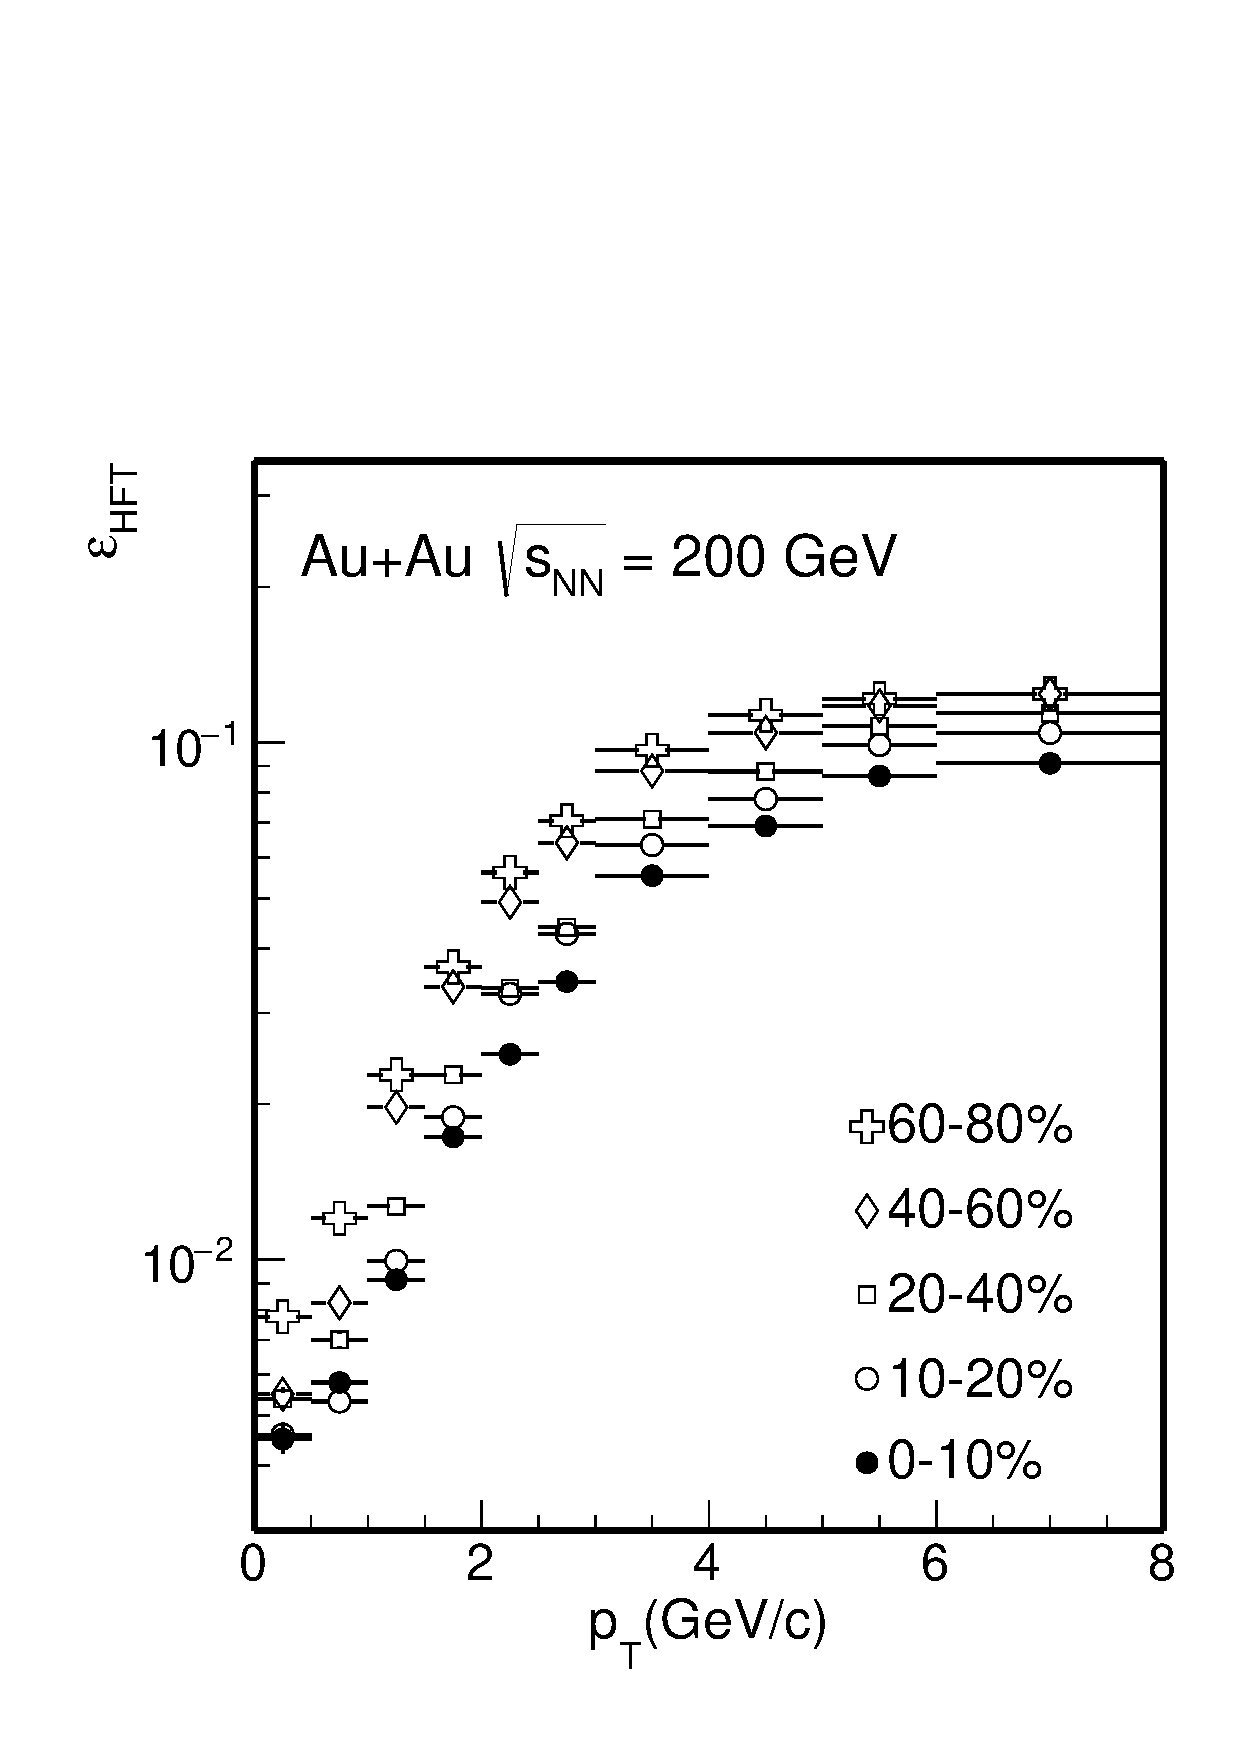
\includegraphics[width=1.0\textwidth,angle=0]{figure/Run14_D0HFT/Datad0Eff_hftTopo.pdf}
\caption{ $D^0$ efficiency step by step from HFT acceptance tracking and topological cuts in different centralities. \label{D0effStep3}}
\end{minipage}
\hfill
\begin{minipage}[htbp]{0.52\linewidth}
\centering
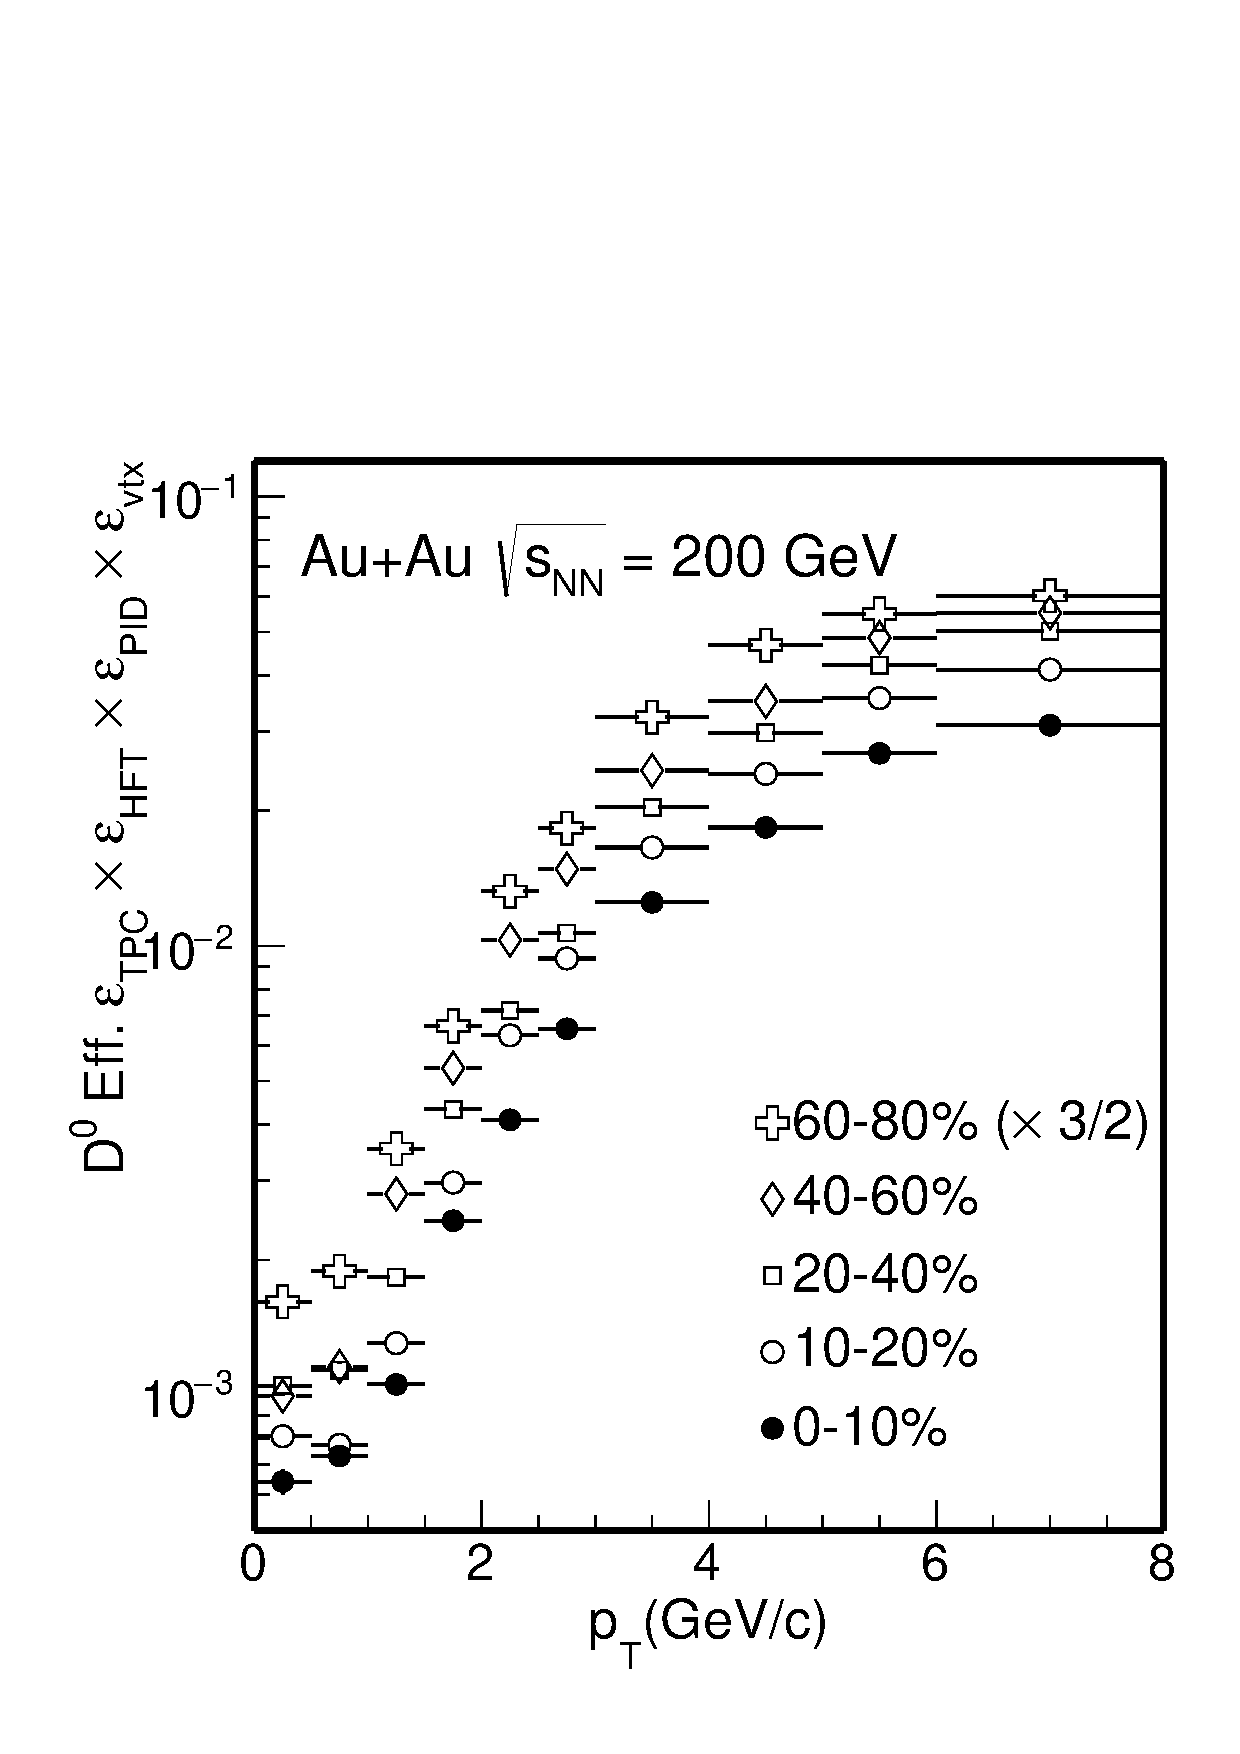
\includegraphics[width=1.0\textwidth,angle=0]{figure/Run14_D0HFT/Datad0Eff.pdf} 
\caption{ $D^0$ efficiency including PID in several centralities. \label{D0effCombine}}
\end{minipage}
\end{figure}

We study all the efficiencies with small centrality bin width, in total we have 9 centrality bins from our StRefmultCorr class. Since the $D^0$ production is scaled by the number of binary collisions ($\textup{N}_{\textup{bin}}$), the $D^0$ is favor produced in more central collisions. So the final efficiencies for the wider centrality bins 0-10\%, 10-40\%, 40-80\% and 0-80\% are calculated using $\textup{N}_{\textup{bin}}$ as weights, for example, the efficiency in 0-80\% is calculated as the following Eq.~\ref{effcombine}. Fig~\ref{D0effCombine} shows the $D^0$ efficiency for 4 wide centralities after TPC, HFT match and Topological efficiency included.

\begin{equation}
  \textup{Efficiency}_{0-80\%} = \sum_{i=1}^{9}(\textup{Efficiency}_{i} \times N_{bin}^{i}) / <\textup{N}_{\textup{bin}}>
\label{effcombine}
\end{equation}

The Data-Driven Fast-Simulation also provide the topological information, can be used for the comparison with real data. For the real data part, within the $D^0$ mass window we can statistical subtract the background and extract the pure $D^0$ topological distributions. The invariant mass plots shown as Fig.~\ref{d0massforTopo}. $D^0$ is in the 2 < $p_T$ < 3 GeV/$c$, 0-80\% centrality. Black is unlikesign foreground, blue is likesign background and red is mixed event background. The blue vertical lines are the mass window used for the topological comparison. For each topological variable, that corresponding topological cut was removed when reconstruct the $D^0$ candidate, so that we can compare that variable in a wide range.

\begin{figure}[htbp]
\centering
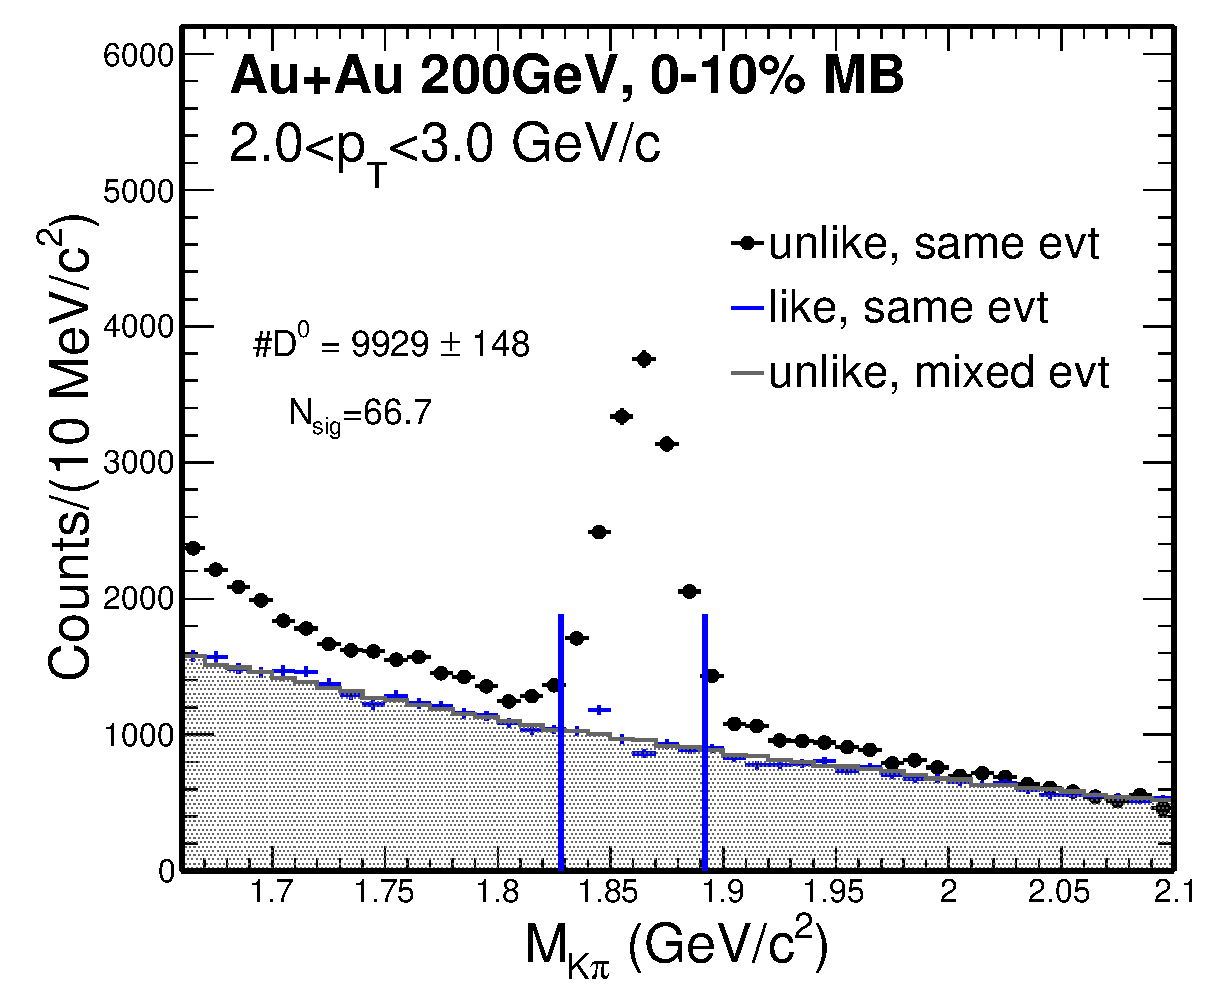
\includegraphics[keepaspectratio,width=0.6\textwidth]{figure/Run14_D0HFT/Mixed_cent_8_9_pt_2_3.eps}
\caption{$D^0$ invariant mass distributions in the 2 < $p_T$ < 3 GeV/$c$, 0-10\% centrality. Black is unlikesign foreground, blue is likesign background and red is mixed event background. The blue vertical lines are the mass window used for the topological comparison.}
\label{d0massforTopo}
\end{figure}

\begin{figure}[htbp]
\begin{minipage}[htbp]{0.52\linewidth}
\centering
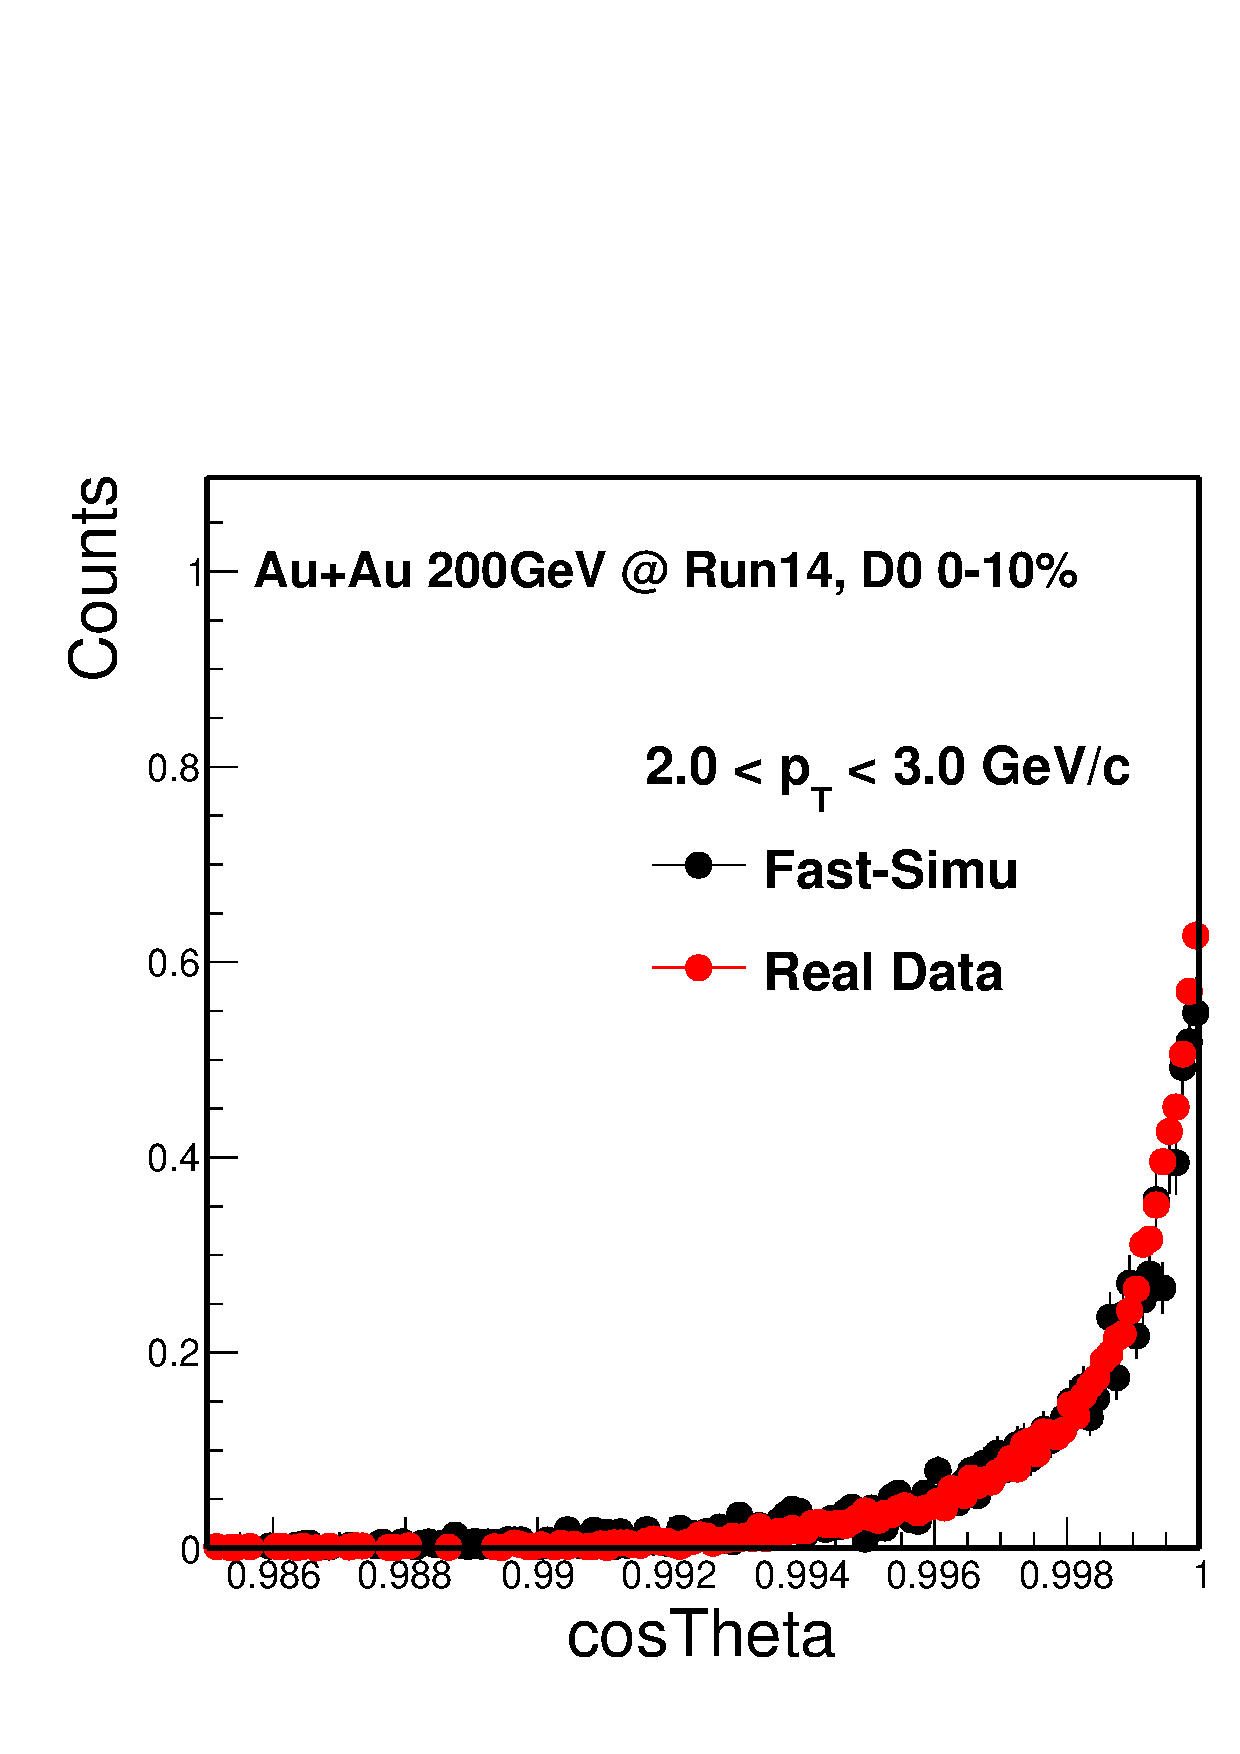
\includegraphics[width=1.0\textwidth,angle=0]{figure/Run14_D0HFT/pointingangle.pdf}
\caption{ $D^0$ cosTheta distribution in most central 0-10\% between Fast-Simulation and Real Data.\label{pointingangle}}
\end{minipage}
\hfill
\begin{minipage}[htbp]{0.52\linewidth}
\centering
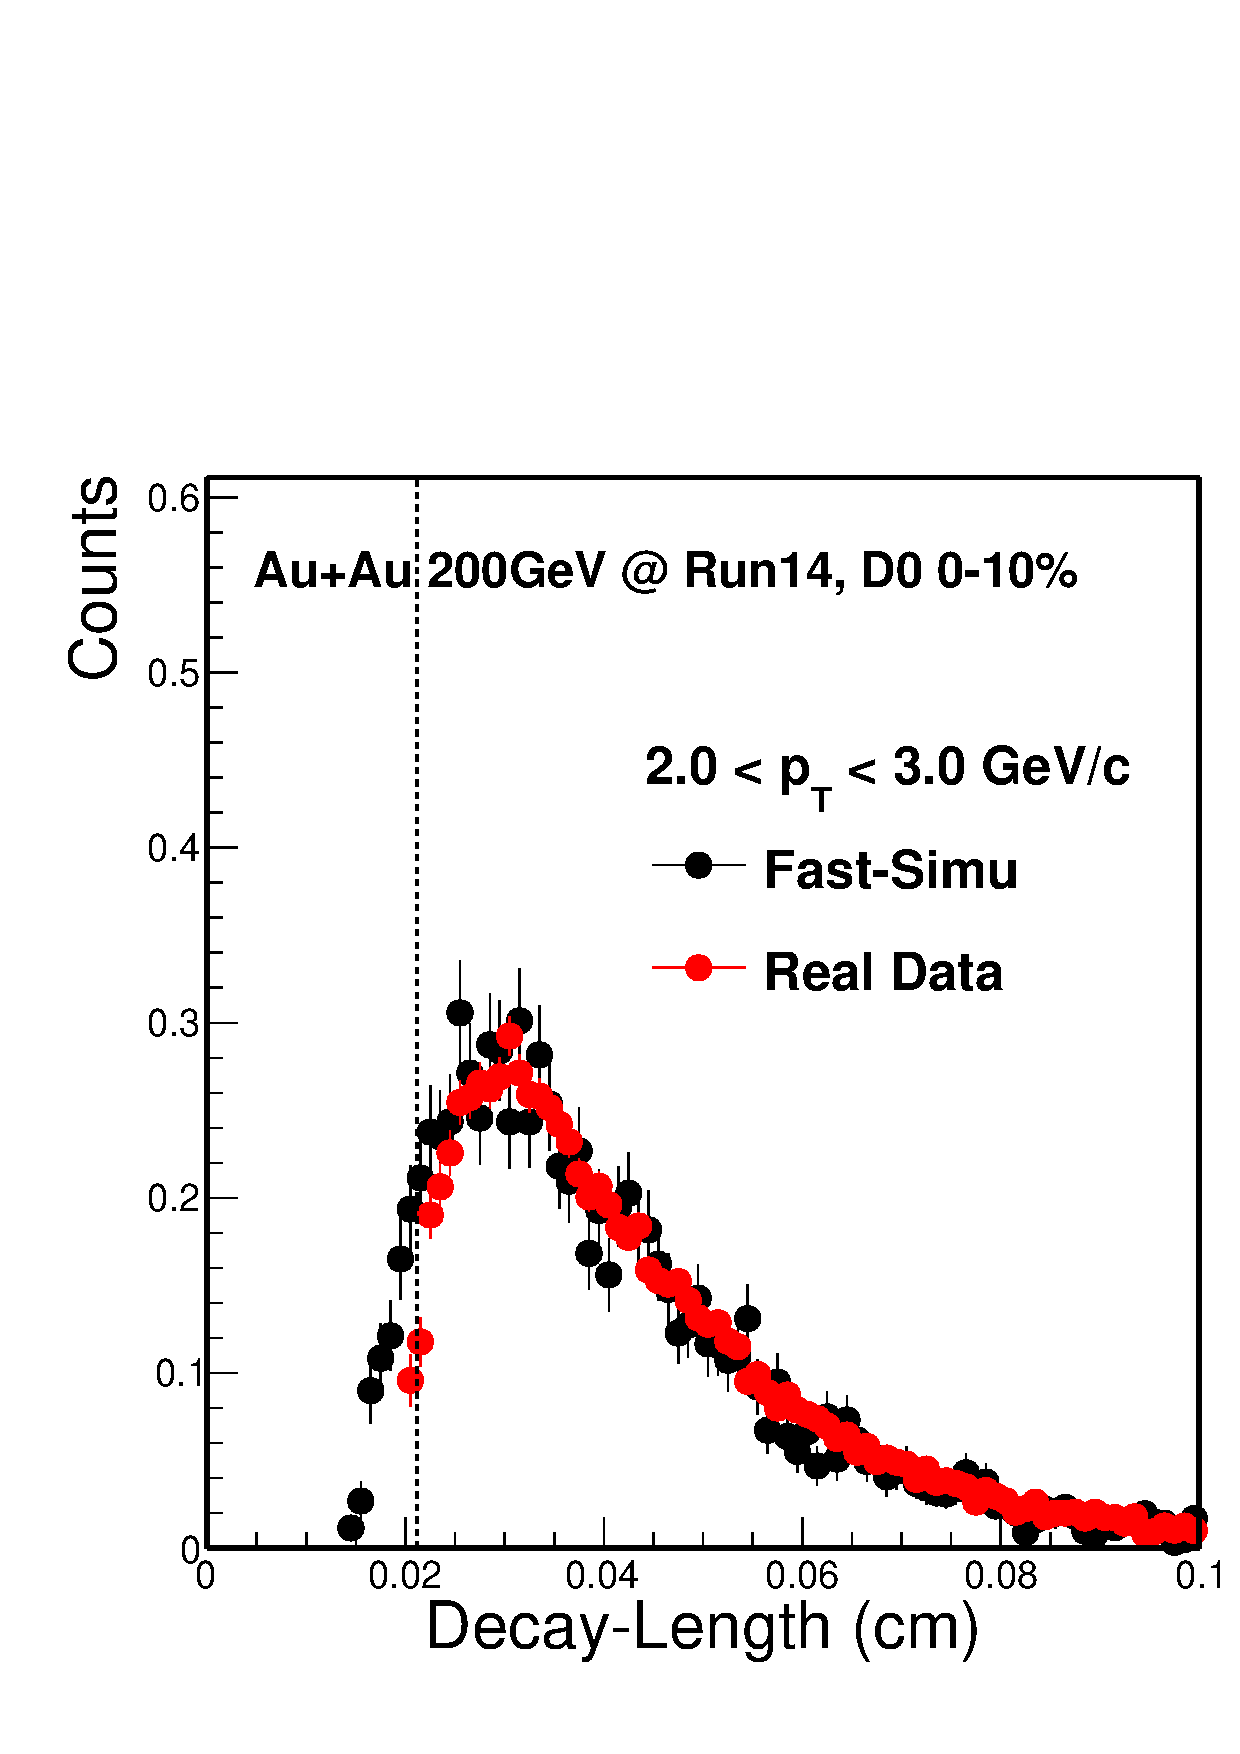
\includegraphics[width=1.0\textwidth,angle=0]{figure/Run14_D0HFT/DecayL.pdf} 
\caption{ $D^0$ decay length distribution in most central 0-10\% between Fast-Simulation and Real Data.\label{DecayL}}
\end{minipage}
\end{figure}

\begin{figure}[htbp]
\begin{minipage}[htbp]{0.52\linewidth}
\centering
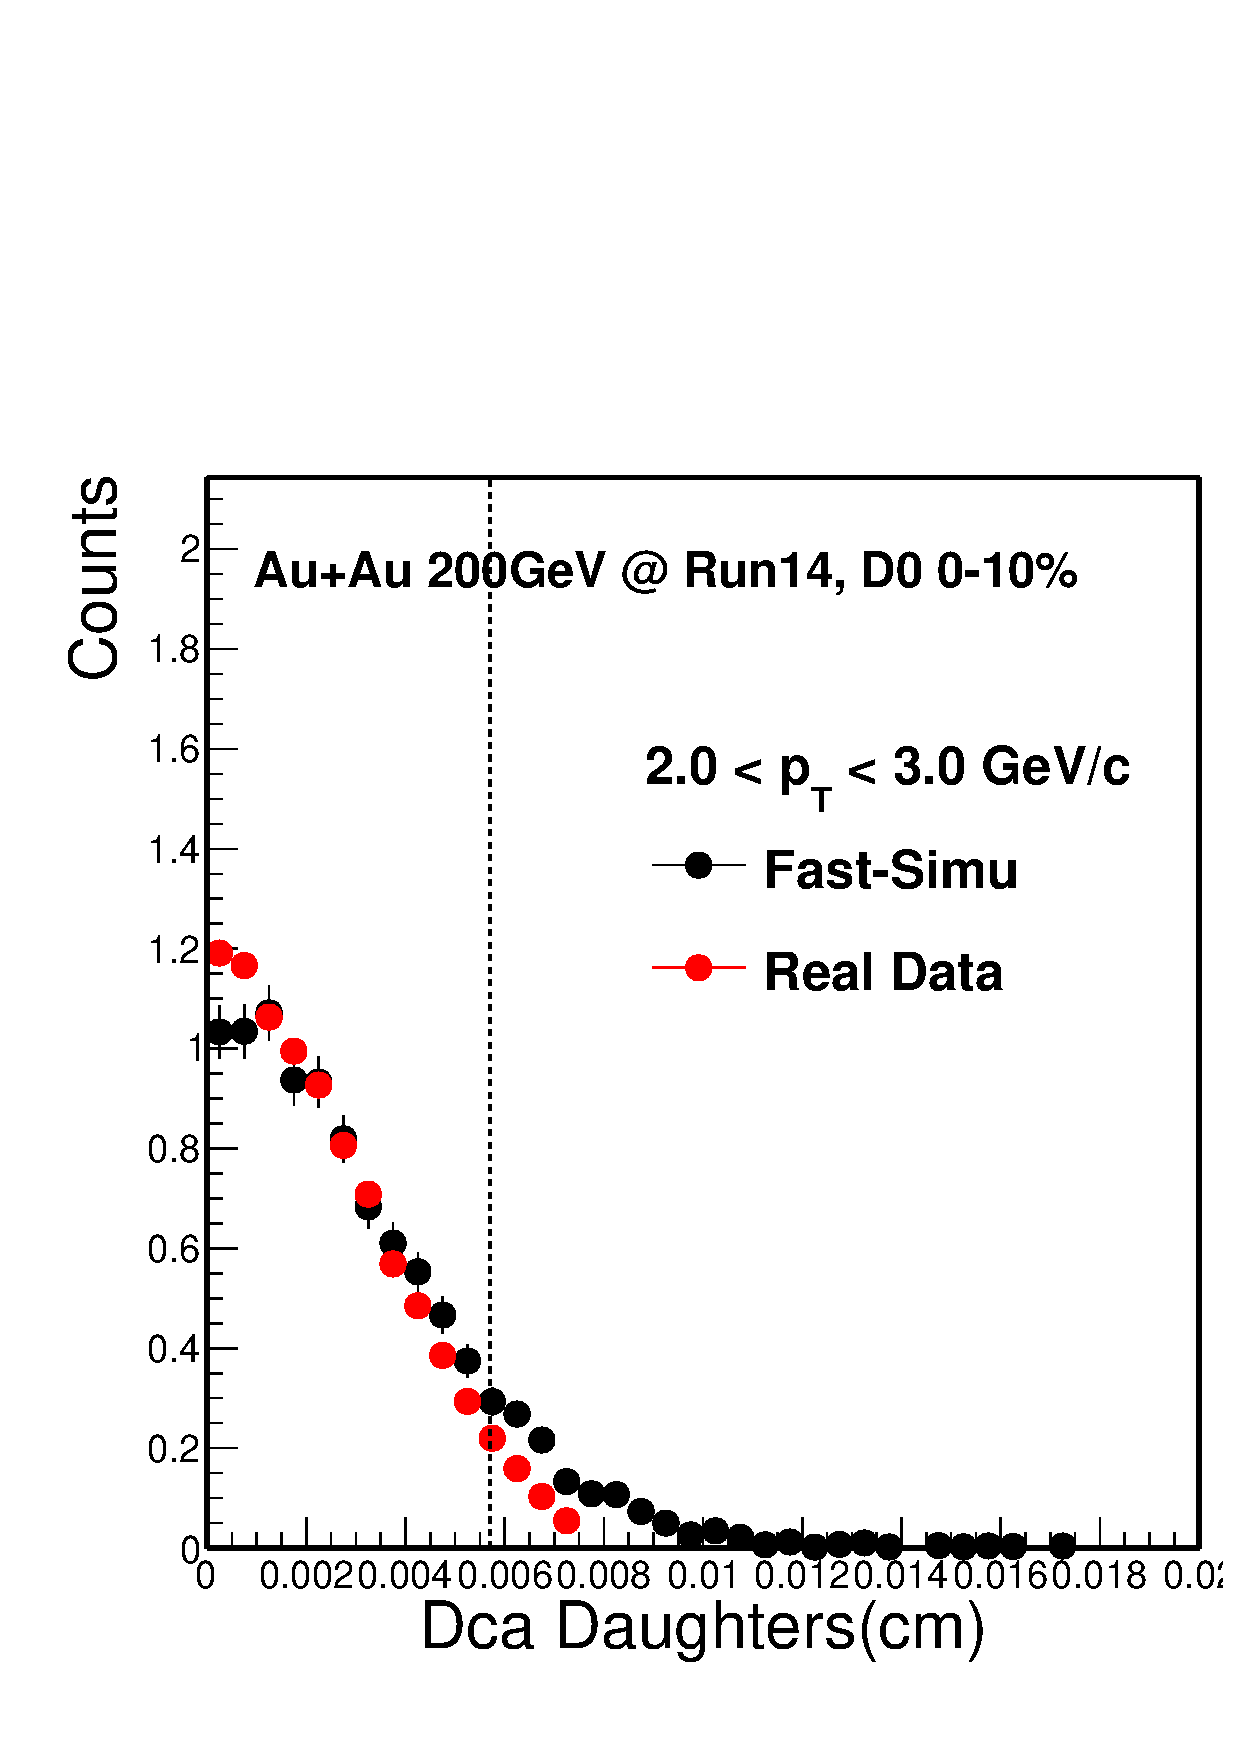
\includegraphics[width=1.0\textwidth,angle=0]{figure/Run14_D0HFT/dcaDaughters.pdf}
\caption{ $D^0$ dcaDaughters distribution in most central 0-10\% between Fast-Simulation and Real Data.\label{dcaDaughters}}
\end{minipage}
\hfill
\begin{minipage}[htbp]{0.52\linewidth}
\centering
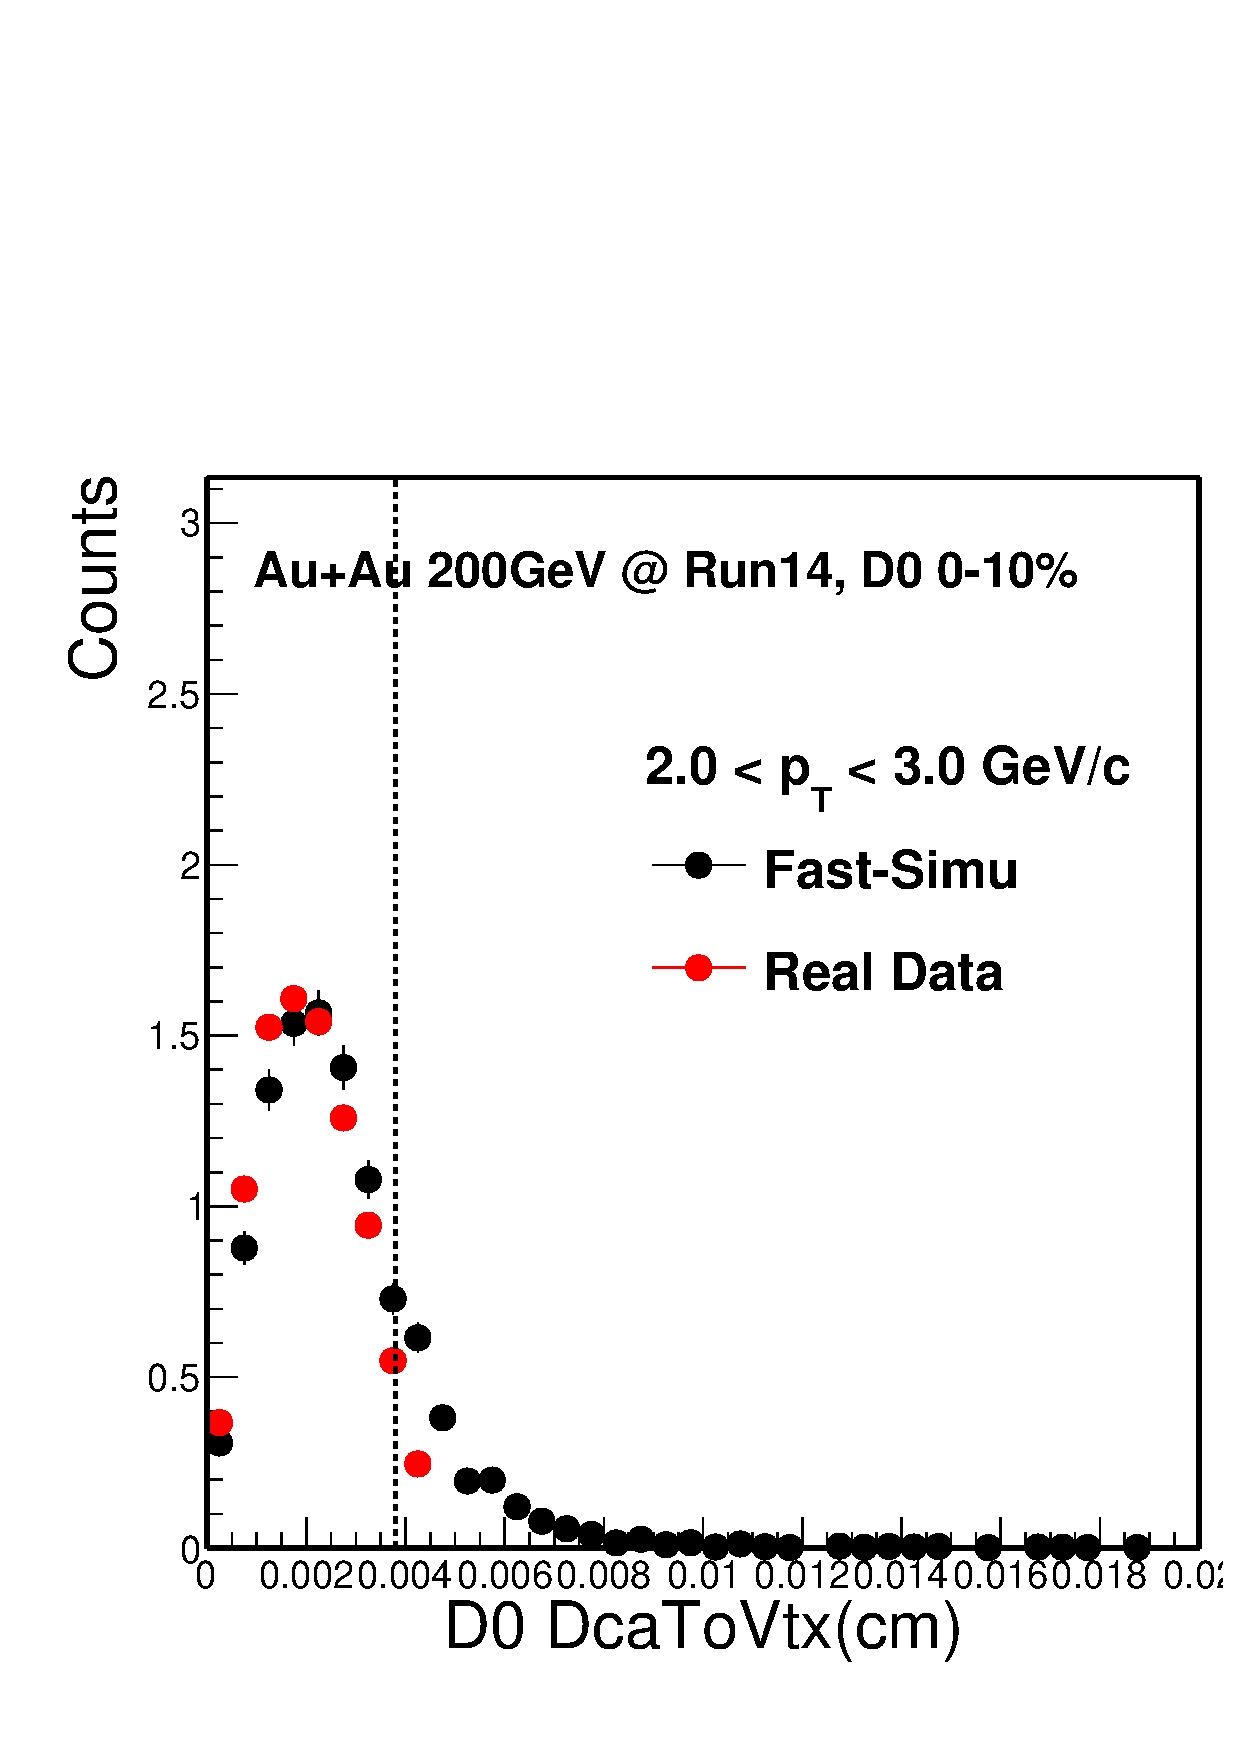
\includegraphics[width=1.0\textwidth,angle=0]{figure/Run14_D0HFT/D0Dca2Vtx.pdf} 
\caption{ $D^0$ dca to Vertex distribution in most central 0-10\% between Fast-Simulation and Real Data.\label{D0Dca2Vtx}}
\end{minipage}
\end{figure}

\begin{figure}[htbp]
\begin{minipage}[htbp]{0.52\linewidth}
\centering
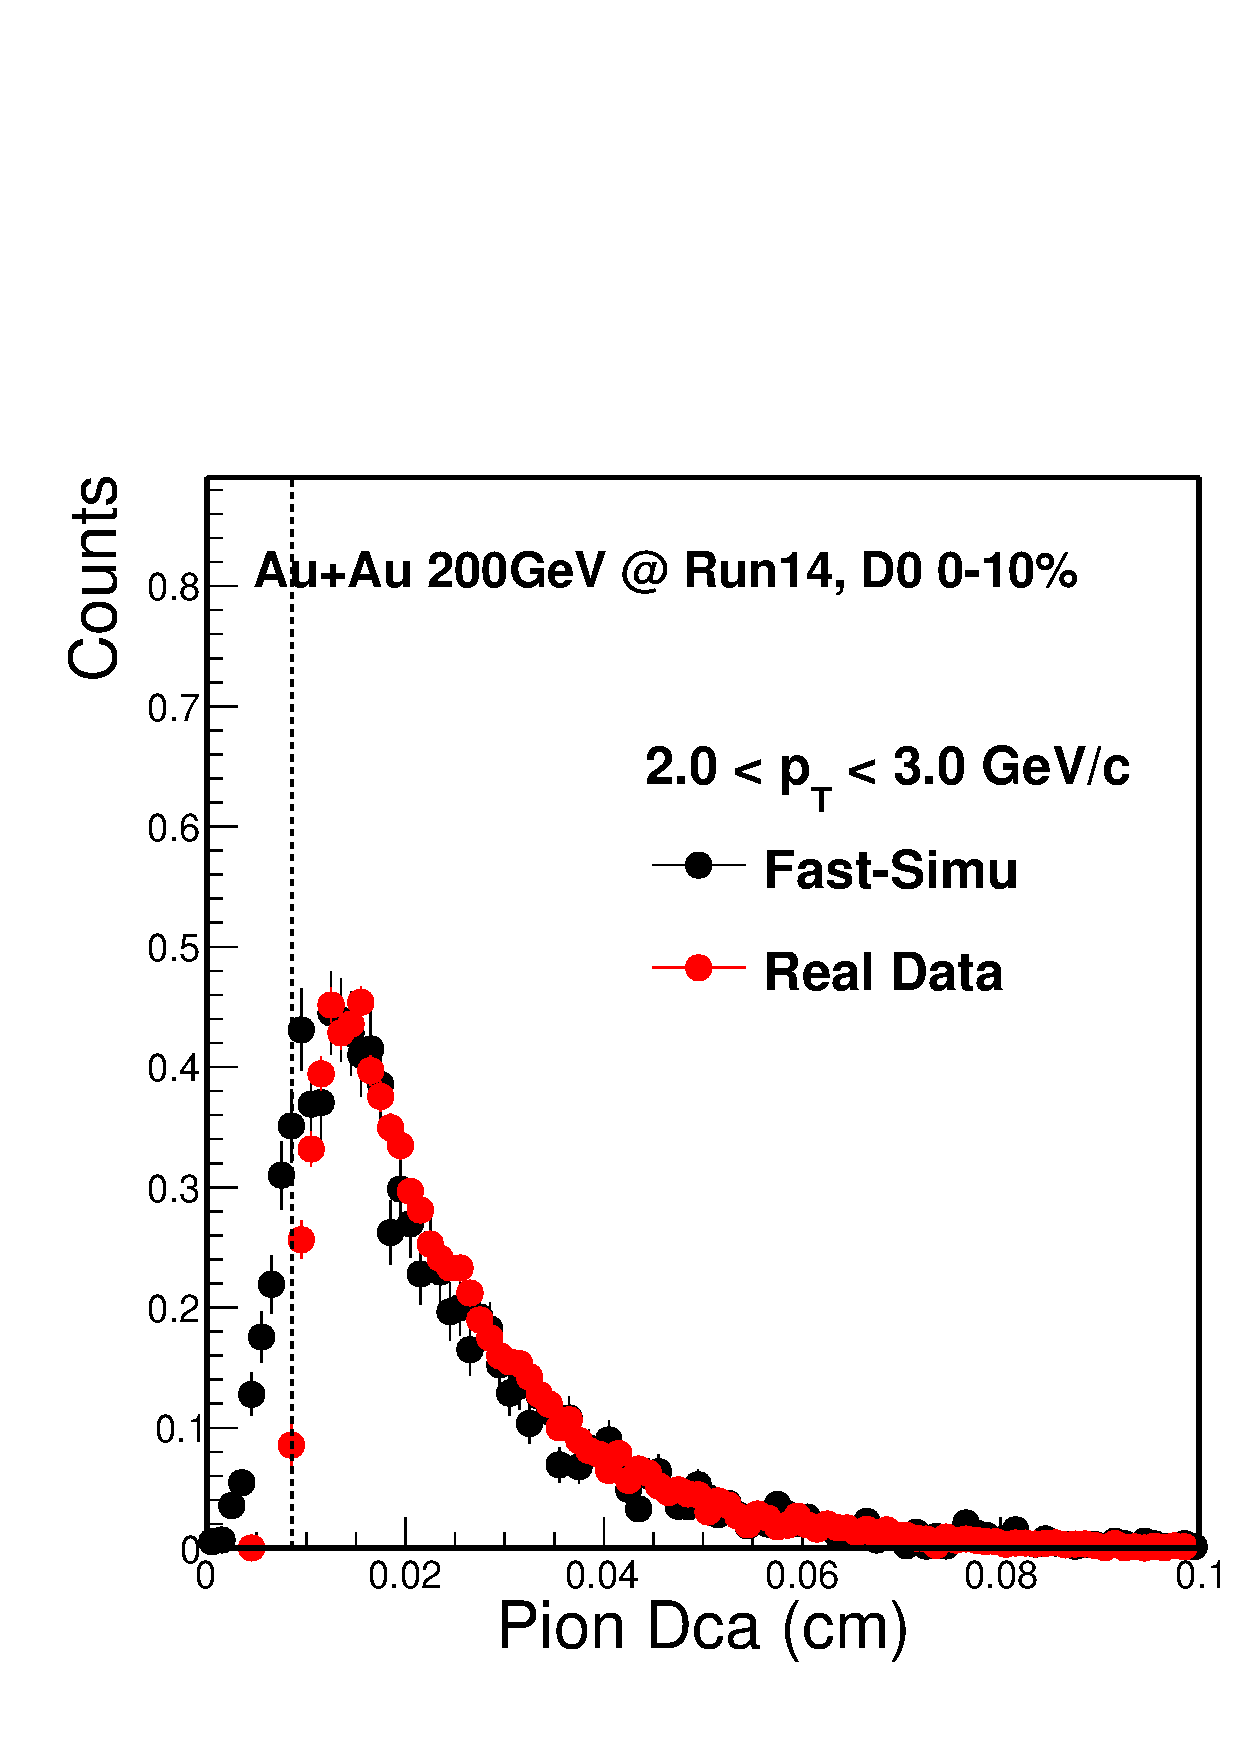
\includegraphics[width=1.0\textwidth,angle=0]{figure/Run14_D0HFT/pionDca.pdf}
\caption{ $D^0$ pionDca distribution in most central 0-10\% between Fast-Simulation and Real Data. \label{pionDca}}
\end{minipage}
\hfill
\begin{minipage}[htbp]{0.52\linewidth}
\centering
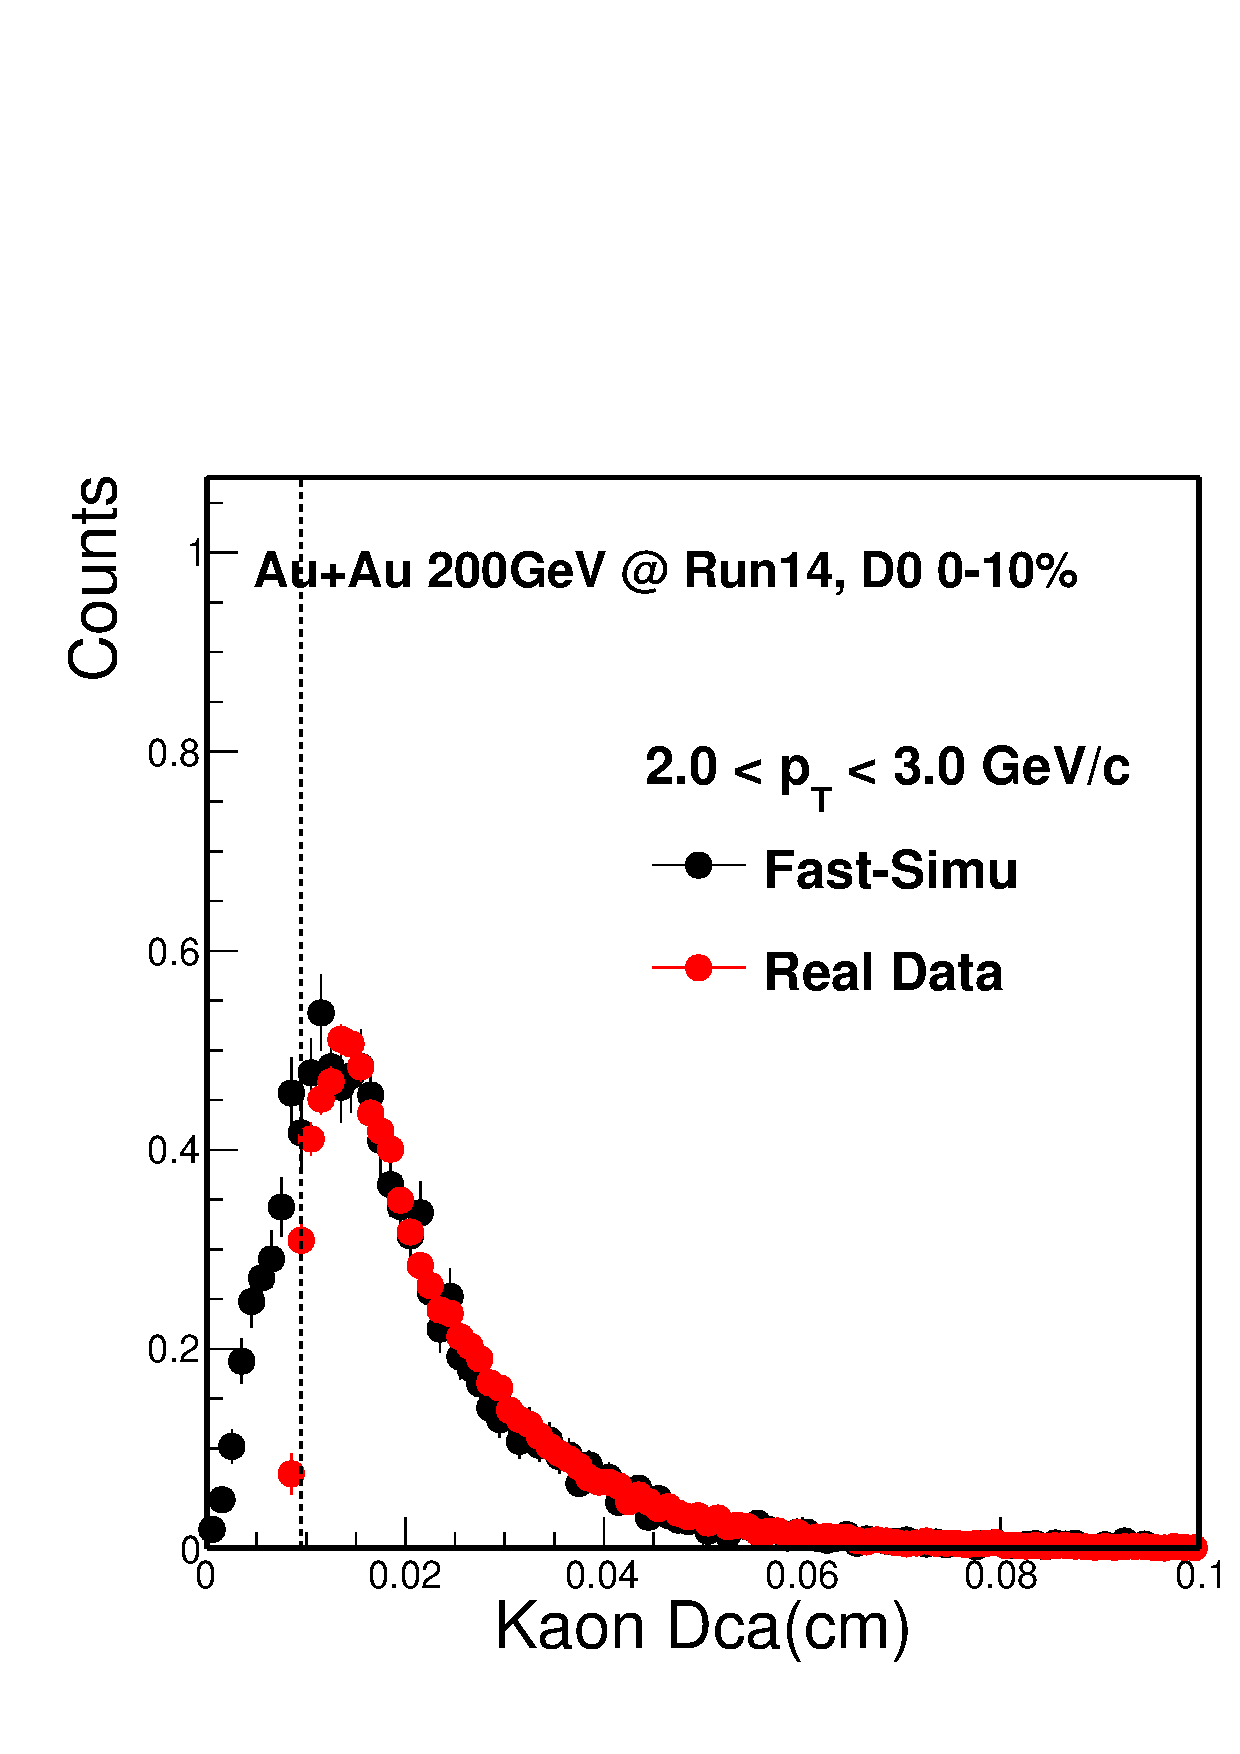
\includegraphics[width=1.0\textwidth,angle=0]{figure/Run14_D0HFT/kaonDca.pdf} 
\caption{ $D^0$ kaonDca distribution in most central 0-10\% between Fast-Simulation and Real Data. \label{kaonDca}}
\end{minipage}
\end{figure}

From Fig.~\ref{pointingangle} to Fig.~\ref{kaonDca}, these are the topological variables (cos($\theta$), decayLength, dcaDaughters, D0DcaToVtx, PionDca and KaonDca) used for the $D^0$ reconstruction. The distributions from the real data part are using mixed event method to statistical subtract the background. The Data-Driven Fast-Simulation part was the package we relayed on for our efficiency study as shown before.

Comparison these topological variables between real data and Fast-Simulation, the agreement is reasonable good, which means our Data-Driven Fast-Simulation method can well reproduce the topological variables in real data. In another word, the efficiency estimation from Data-Driven Fast-Simulation is reliable. Note here, there are some small discrepancy such as single track Dca distributions in the low end, that's because in the data analysis part, we already require some minimum cut in order to save the computing resource. There is another method we are going to discuss in the following section, also can be used to validating our Fast-Simulation method.

\subsection{Validation with Full GEANT+Hijing Simulation}

Before discuss the details of this Hijing validation, it's better to conclude those assumptions we made before. The first assumption is the factorization shown in Eq.~\ref{efffact}. Relaying on the Hijing simulation, we have two samples. One is only include TPC tracking, another one include both HFT and TPC in tracking. From the first sample, we can extract the TPC factorized tracking efficiency, and the second sample can be used to extract the overall total efficiency and HFT over TPC factorized efficiency separately. Fig.~\ref{assumption01} shows the comparison between the overall efficiency and the multiplied factorization efficiency. The red one is from overall efficiency from the second sample, and the blue one is multiplied efficiency from two components. The bottom panel shows the double ratio of these two efficiency, and they are perfectly factorized as the ratio is flat as unity.

\begin{figure}[htbp]
\centering
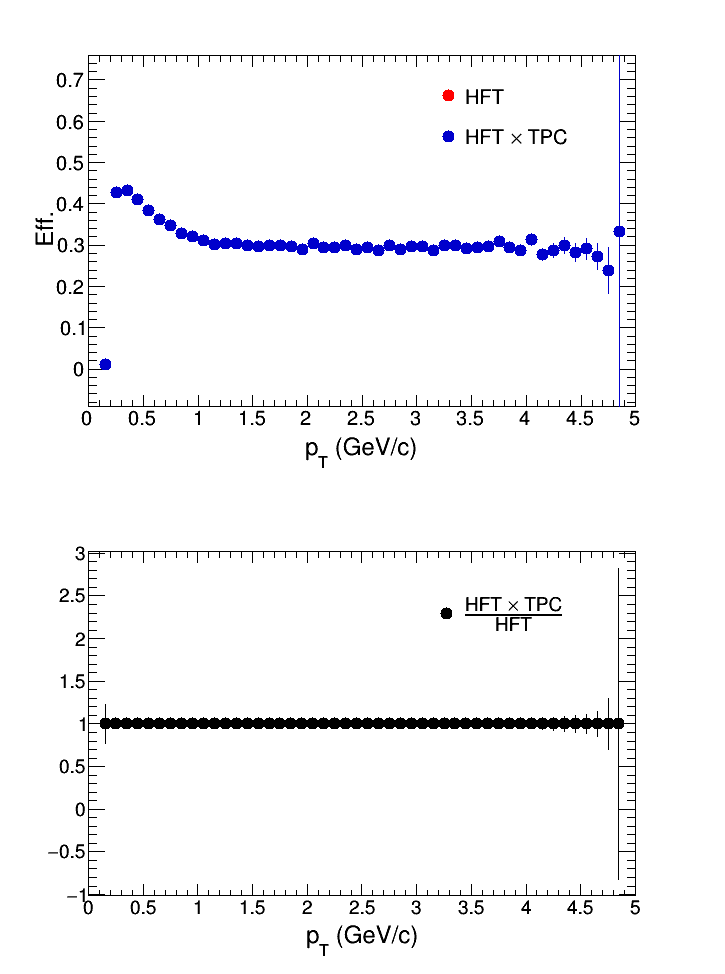
\includegraphics[keepaspectratio,width=0.7\textwidth]{figure/Run14_D0HFT/assumption01.png}
\caption{(top)HFT Efficiency Factorization comparison. (bottom) Double Ratio of these factorization.}
\label{assumption01}
\end{figure}

The second assumption is for the spatial resolution, it is encoded in those $\textup{Dca}_{\textup{XY}}$ and $\textup{Dca}_{\textup{Z}}$ variables, and they are correlated in the two dimensions. Fig.~\ref{assumption2} shows the comparison between the input Dca from real data and output Dca from Fast-Simulation in three dimensions. The first row is Dca in XY plane, the second row is in Z plane and the last row is in the 3-D dimension. From the left to right is the comparison from low $p_{T}$ to high $p_{T}$. As shown the red line is from data and black line is from fast simulation, the agreement is pretty good.
For the others assumption, they will be discussed separately in the following section.

\begin{figure}[htbp]
\centering
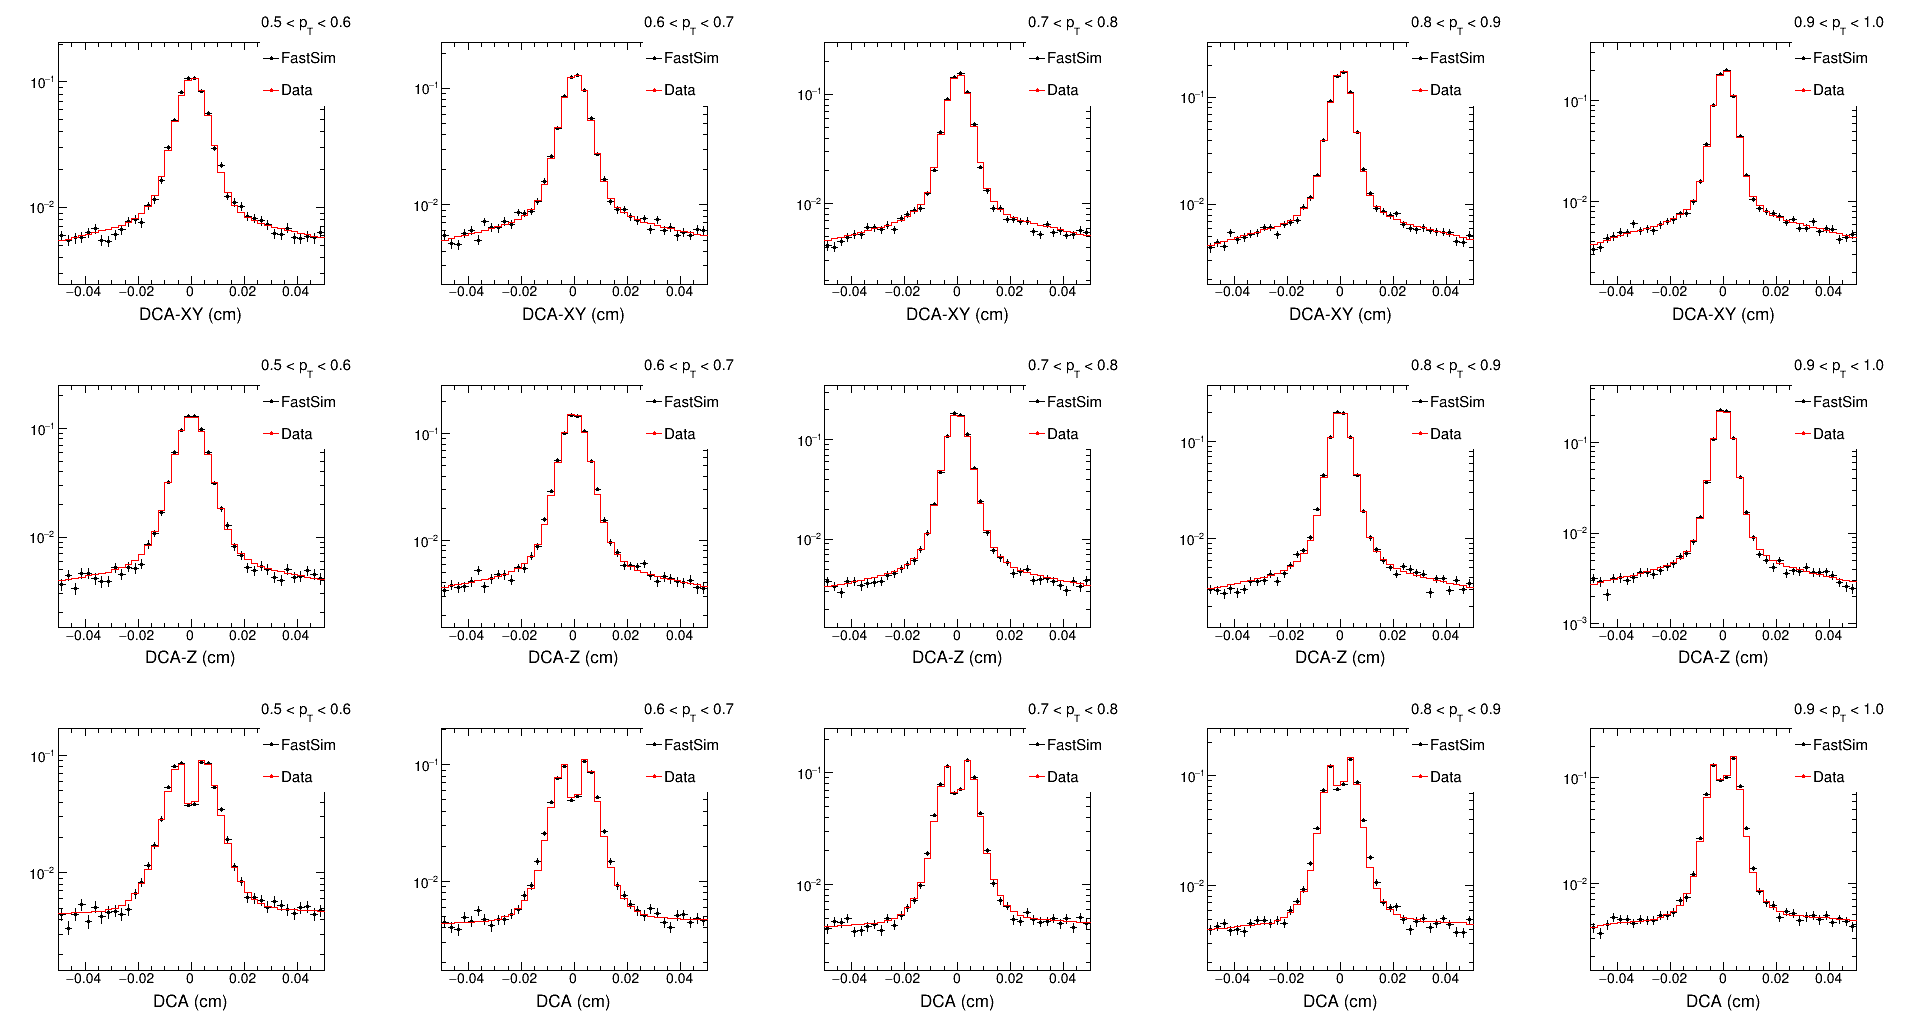
\includegraphics[keepaspectratio,width=1.0\textwidth]{figure/Run14_D0HFT/assumption2.png}
\caption{Comparison of Dca between data (red) and Fast-Simulation (black). From top to bottom, the comparison is for $\textup{Dca}_{\textup{XY}}$, $\textup{Dca}_{\textup{Z}}$ and $\textup{Dca}$. From left to right the transverse momentum is from low $p_T$ to high $p_T$.}
\label{assumption2}
\end{figure}

\subsection{Hijing Samples Performance}
\label{hijingsample}
The Hijing sample was run through the Full Hijing + GEANT simulation with realistic pileup hits (UPC+MB) in PXL and sensor masking tables. They can provide reasonable performance for the HFT matching ratio and Dca resolution. 
In total we have $\sim$45K 0-10\% centrality Hijing events, and for each event is embedded with 20 $D^0$'s. So in total, we have $\sim$900K $D^0$ for this Hijing sample. The embedded $D^0$ has small effect on the tracking since the multiplicity is much higher compared to 20 $\times$ 2 $D^0$' decayed daughters.

\begin{figure}[htbp]
\begin{minipage}[htbp]{0.52\linewidth}
\centering
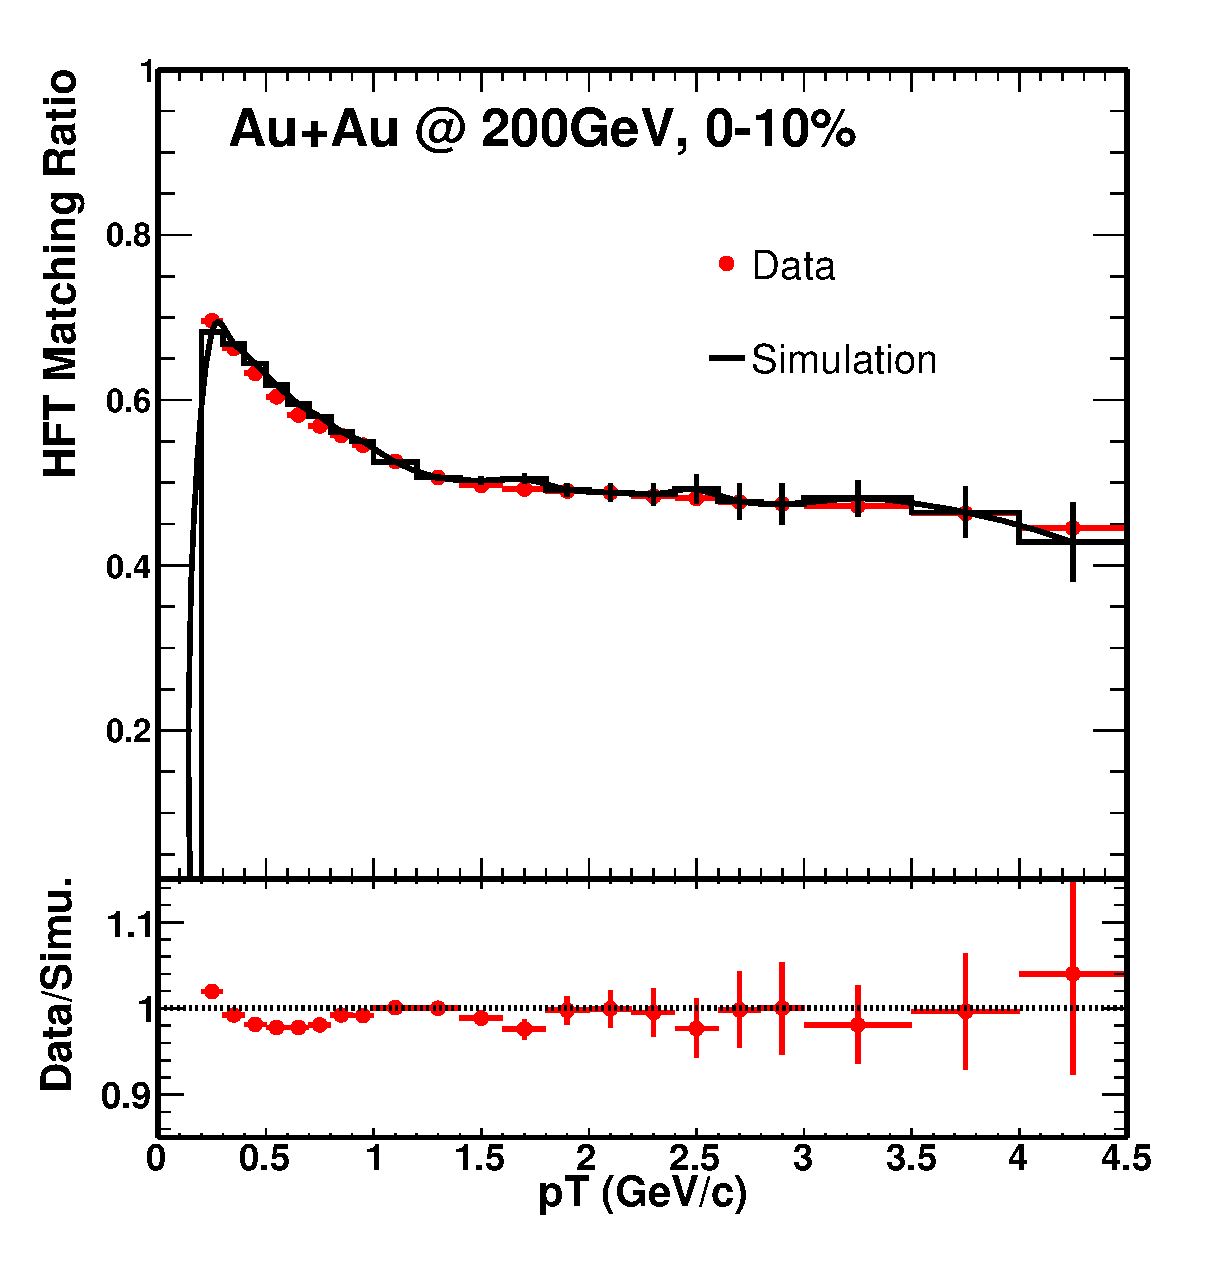
\includegraphics[width=1.0\textwidth,angle=0]{figure/Run14_D0HFT/HijingRatio.eps}
\caption{ HFT Ratio comparison between data and Hijing simulation in Au+Au 200 GeV/c, 0-10\%.\label{HijingRatio}}
\end{minipage}
\hfill
\begin{minipage}[htbp]{0.52\linewidth}
\centering
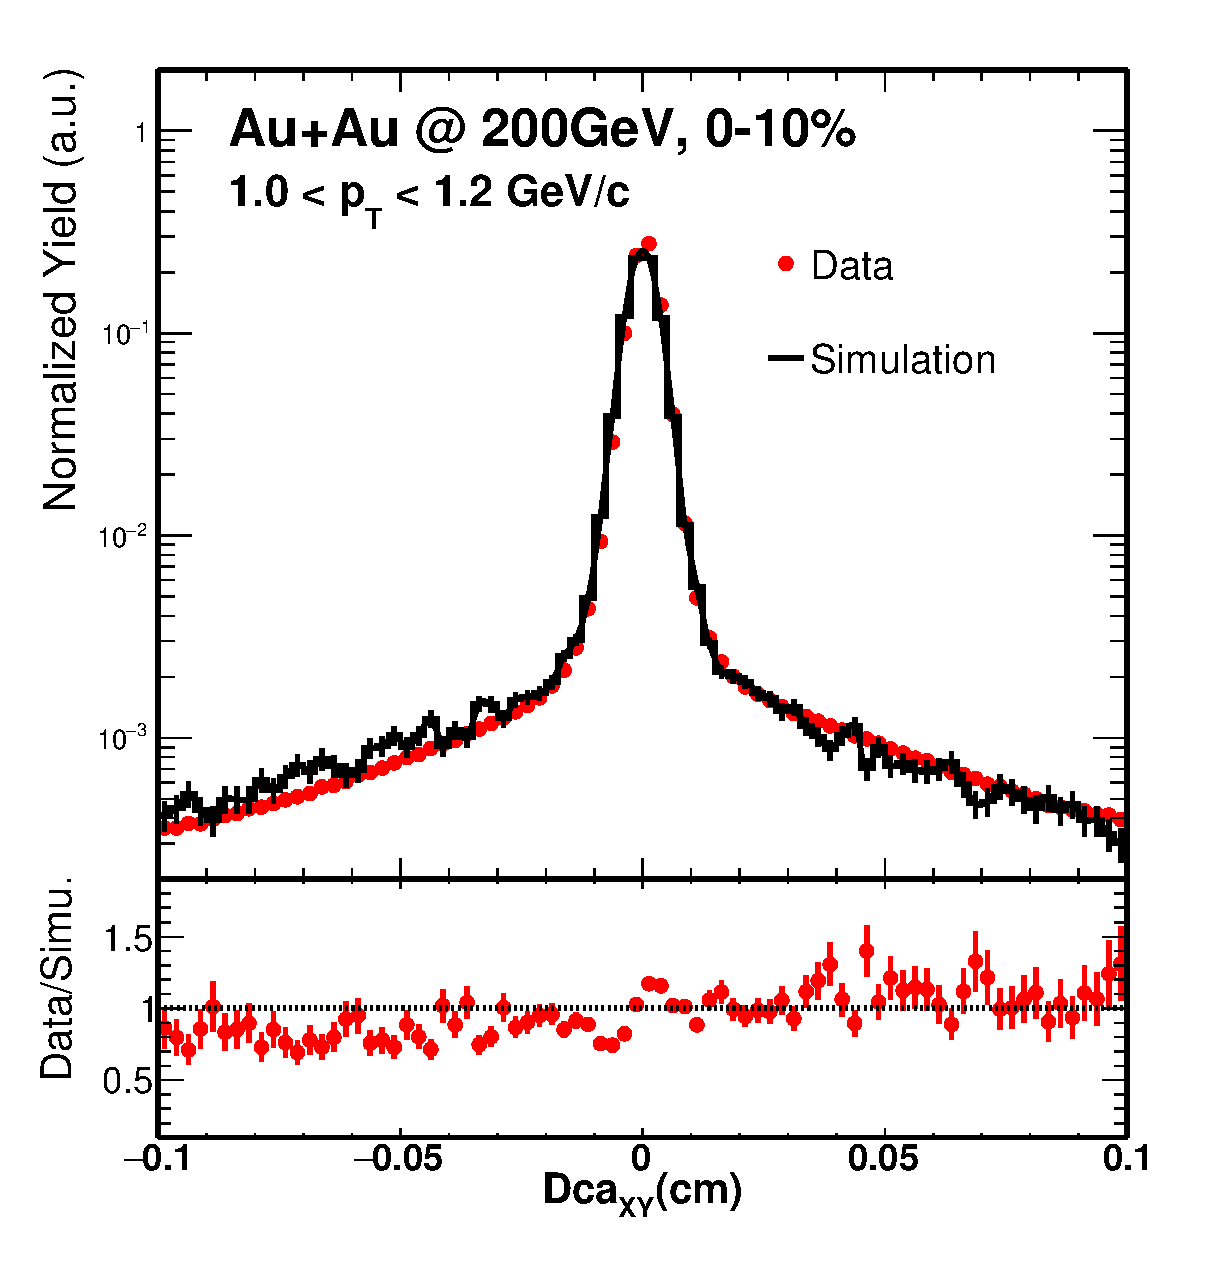
\includegraphics[width=1.0\textwidth,angle=0]{figure/Run14_D0HFT/HijingDca.eps} 
\caption{ $\pi^{\pm}$ $\textup{Dca}_{\textup{XY}}$ comparison between data and Hijing simulation in Au+Au 200 GeV/c, 0-10\%.\label{HijingDca}}
\end{minipage}
\end{figure}

As shown in Fig.~\ref{HijingRatio} is the HFT matching ratio comparison between data (red) and Hijing samples (black) in Au+Au 200 GeV/$c$ from 0-10\% centrality, the bottom panel is the double ratio of these two HFT matching ratio. The value is around unity, which means the Hijng simulation can well reproduce these matching performance. 

Fig.~\ref{HijingDca} shows the pions $\textup{Dca}_{\textup{XY}}$ comparison between data (red) and Hijing samples (black) in Au+Au 200 GeV/$c$ from 0-10\% centrality at 1.0 < $p_T$ < 1.2GeV/$c$, the bottom panel is the double ratio of these two Dca distributions. The value is also around unity, which means the Hijng simulation well describes the real data.

\subsection{Validation Procedures}
\label{validationprocedure}

The idea is simple for this Hijing validation, we have the enriched $D^0$ Hijing sample. After run through the detector and full GEANT simulation, the $D^0$ efficiency and topological variables distributions can be extracted. Another procedure is extract the necessary ingredients from Hijng sample for the Fast-Simulation input (Fast-Simulation with Hijing input), such as the TPC Tracking efficiency, the HFT matching ratio and the 2D $\textup{Dca}_\textup{XY}$-$\textup{Dca}_\textup{Z}$ distributions similar as we used in real data analysis and discussed in the previous section. Then run through the Fast Simulation, as discussed before, the $D^0$ efficiency and topological variables are also available in this way and can be compared to the first Hijing + GEANT procedure. The workflow is shown in Fig.~\ref{validation0}.

\begin{figure}[htbp]
\centering
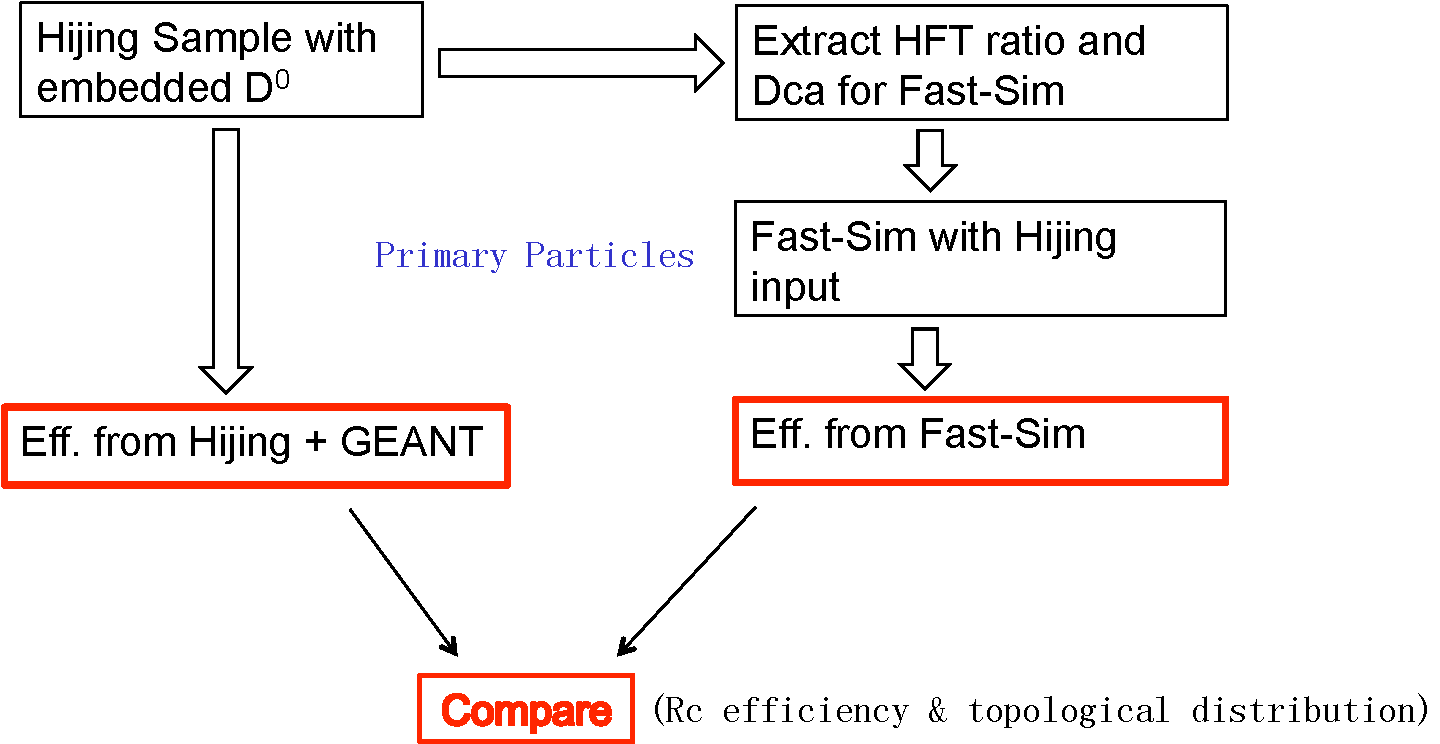
\includegraphics[keepaspectratio,width=1.0\textwidth]{figure/Run14_D0HFT/validation0.pdf}
\caption{Hjiing validation procedure and workflow}
\label{validation0}
\end{figure}

\subsubsection{Validation Efficiency}
\label{validationeff}

The first step is to check the kinematic form different MC decayer such as PYTHIA, Hijing, evtGen and PhaseSpace class from ROOT. Need to make sure the decayer used for Fast-Simulation has the same kinematic as the Hijng. After the basic acceptance cut, such as $D^0$ |y| < 1, daughter $p_T$ > 0.2 GeV/$c$ and |$\eta$| <1 cut. $D^0$ is the simple phase space decay, all these decayer give the same acceptance efficiency as shown in Fig.~\ref{d0decayer} left panel, the right panel shows the double ratio to PYTHIA. As all the decayer follow the same trend they have the same decay kinematic, so, for our Fast-Simulation decayer we choose PYTHIA for this validation and also for our real data analysis.

\begin{figure}[htbp]
\centering
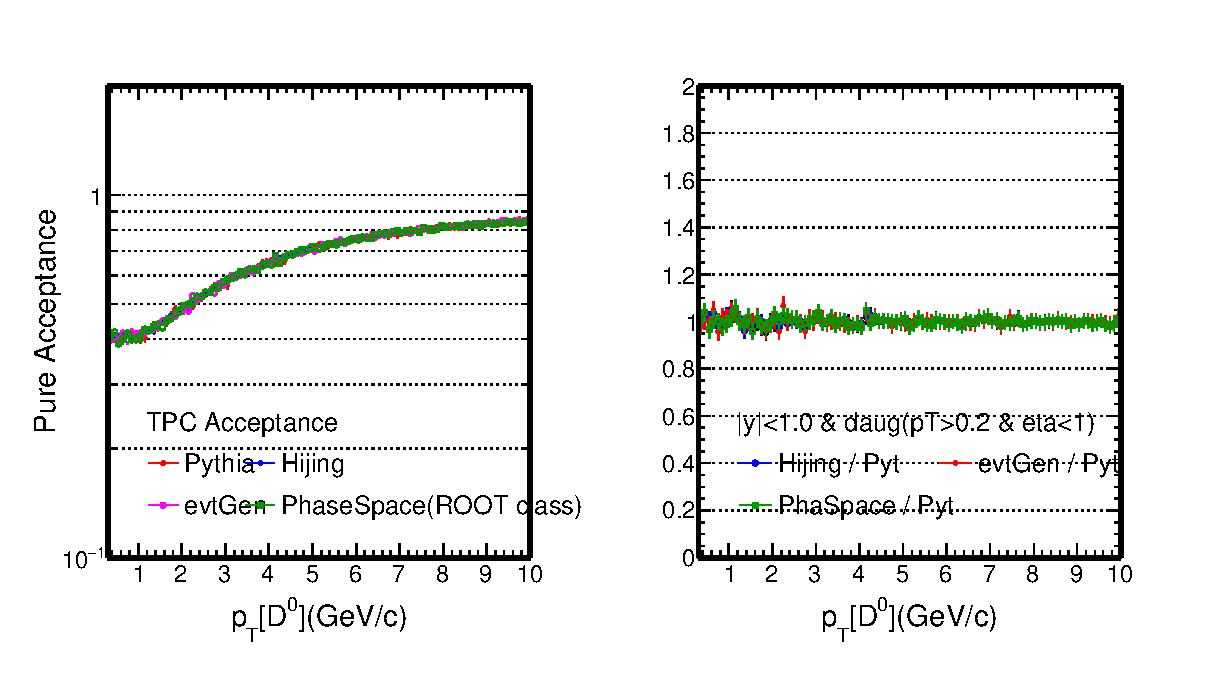
\includegraphics[keepaspectratio,width=1.0\textwidth]{figure/Run14_D0HFT/Acceptance_D0Decayer.eps}
\caption{$D^0$ pure acceptance from different MC decayer, such as PYTHIA, Hijing, evtGen and PhaseSpace class. (right) Double ratio of the acceptance to PYTHIA.}
\label{d0decayer}
\end{figure}

The second step is to check the kinematic with the reconstructed TPC tracking information. Compare to the first step, this one fold in the momentum resolution and the TPC acceptance effect. Fig.~\ref{d0tpceff} left panel shows this efficiency $\times$ Acceptance comparison between Hijing + GEANT (red) and Fast-Simulation with Hijing input (black), the right panel shows the double ratio to Hijing. As the red line is the fit function and the fit results around $\sim$1 shows very good agreement, which means this step is also doing right work.

\begin{figure}[htbp]
\centering
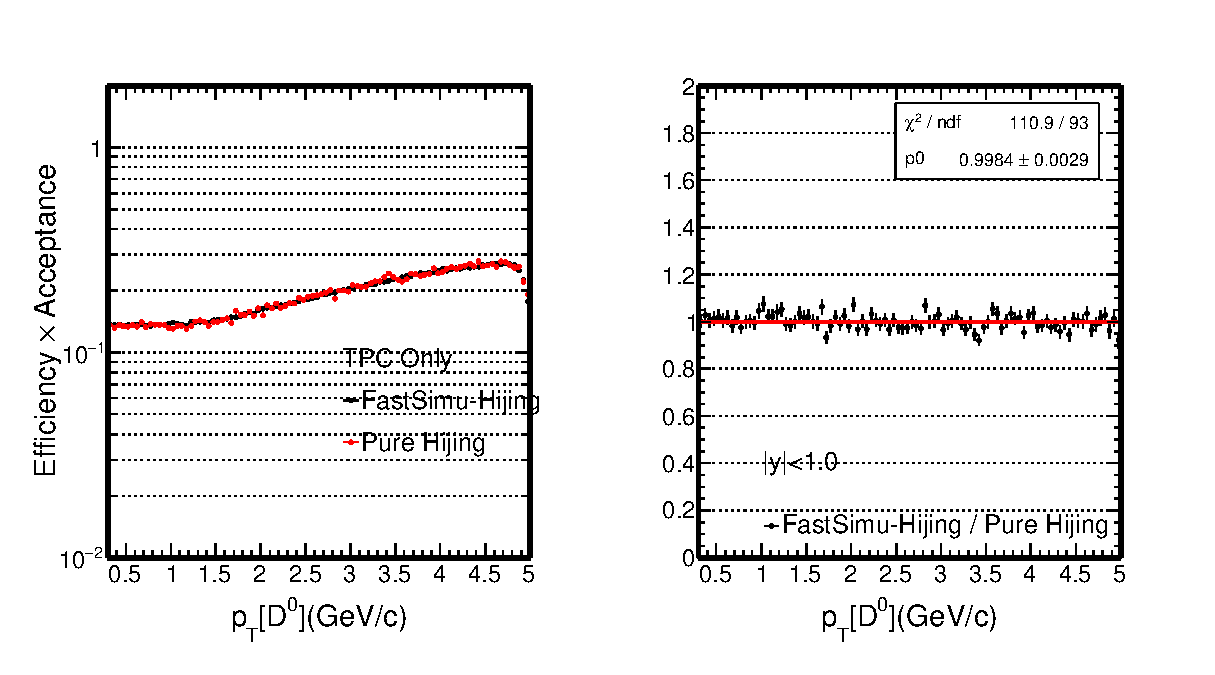
\includegraphics[keepaspectratio,width=1.0\textwidth]{figure/Run14_D0HFT/Physics_FastHijingVsPureHijing_TpcOnly2.eps}
\caption{The comparison of $D^0$ TPC acceptance $\times$ efficiency between Hijing + GEANT (red) and Fast-Simulation with Hijing input (black). (right) Double ratio of these acceptance to Hijing.}
\label{d0tpceff}
\end{figure}

The next step is to trying to fold in the HFT matching efficiency and this is to consider the HFT acceptance effect. Fig.~\ref{d0hftmatcheff} left panel shows this efficiency $\times$ Acceptance comparison after TPC and HFT matching between Hijing + GEANT (red) and Fast-Simulation (black), the right panel shows the double ratio to Hijing. As the red line is the fit function and the fit results around $\sim$1 shows good agreement, which means this HFT matching step is also correctly implemented in the package. For the small discrepancy at the high $p_T$ range, this is purely due to the limited statistics. Since the Hijing sample is time consumption, we do not have enough statistics for the HFT match ratio input. But this problem is not exist for our real data analysis since we have $\sim$900M events which is totally enough and we checked the HFT match ratio, they can extend to a reasonable high $p_T$ range in real data. We did another small check, use one quart of these Hijing statistics for this validation, and the discrepancy shown here is bigger than the current results, which is another approve of the limited Hijing statistics.

\begin{figure}[htbp]
\centering
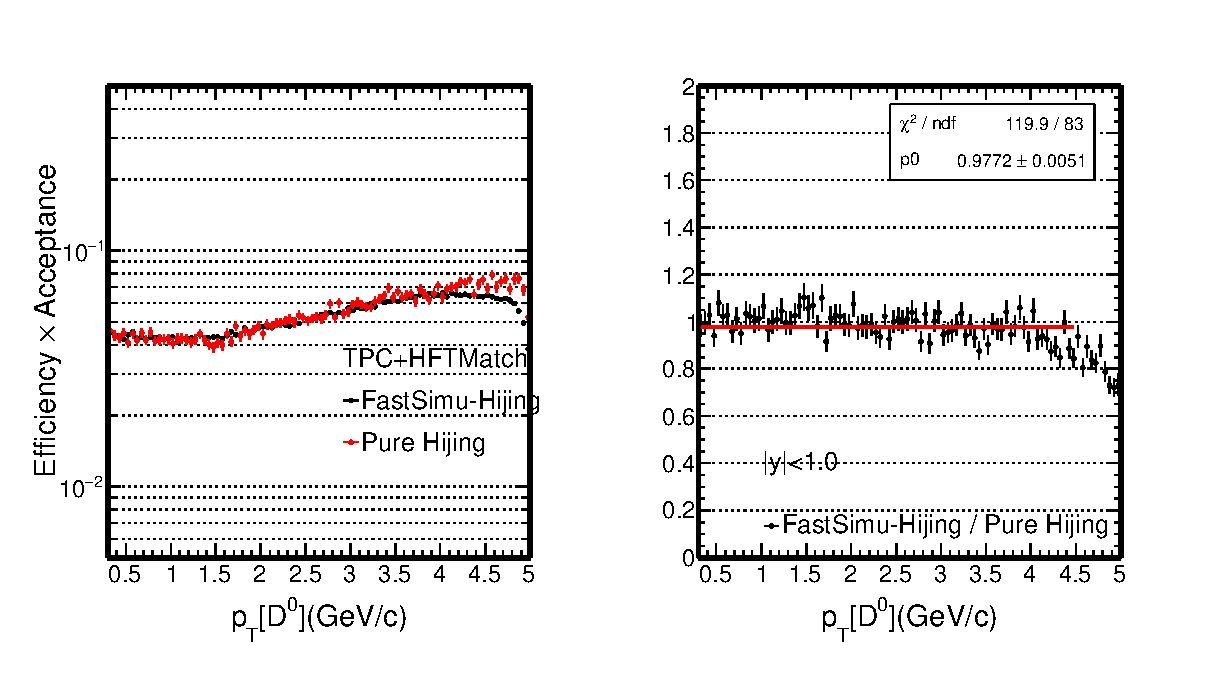
\includegraphics[keepaspectratio,width=1.0\textwidth]{figure/Run14_D0HFT/Physics_FastHijingVsPureHijing_HFTRatio2.eps}
\caption{The comparison of $D^0$ TPC + HFT match acceptance $\times$ efficiency between Hijing + GEANT (red) and Fast-Simulation with Hijing input (black). (right) Double ratio of these acceptance to Hijing.}
\label{d0hftmatcheff}
\end{figure}

The last step is folding in the topological cuts and then compare between the Hijing and Fast-Simulation. Fig.~\ref{d0hfttopoeff} left panel shows this efficiency $\times$ Acceptance comparison after TPC, HFT matching and topological cuts between Hijing + GEANT (red) and Fast-Simulation (black), the right panel shows the double ratio to Hijing. Still the red line is the fit function and the fit results around $\sim$0.93 shows good agreement, which means this topological variables are well described in the package. For the left panel, there are some twist for this efficiency $\times$ acceptance at $p_T$ $\sim$1 GeV/$c$ and 2 GeV/$c$, this is due to the topological cuts are different in separate $p_T$ ranges. As the red points show the efficiency from Hijing + GEANT, the statistics error is larger compared to the Fast-Simulation which shows by black. This is also the reason we use data-driven Fast-Simulation for our efficiency study, it can be easily enlarge the statistics by a factor of 100 or even 1000 compare to the traditional Full GEANT simulation especially for this kind of low efficiency studies. Fig.~\ref{d0hfttopoeff2} shows the same plots of the comparison as Fig.~\ref{d0hfttopoeff} with different binning, we merged some binning for statistics concern. After merged the binning, the agreement is even better from the fitting shown on the right panel, the fitting results is $\sim$0.96.

\begin{figure}[htbp]
\centering
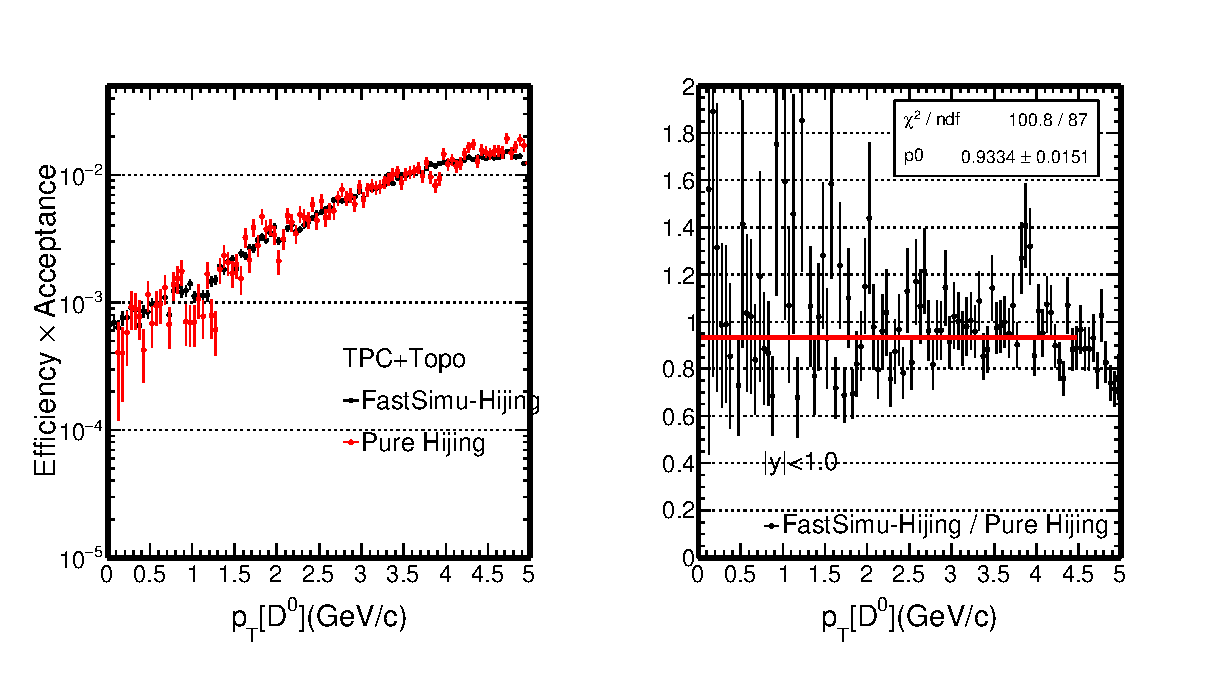
\includegraphics[keepaspectratio,width=1.0\textwidth,angle=0]{figure/Run14_D0HFT/Physics_FastHijingVsPureHijing_HFTTopo2.eps}
\caption{The comparison of $D^0$ TPC + HFT match + Topological acceptance $\times$ efficiency between Hijing + GEANT (red) and Fast-Simulation with Hijing input (black). (right) Double ratio of these acceptance to Hijing.}
\label{d0hfttopoeff}
\end{figure}

\begin{figure}[htbp]
\centering
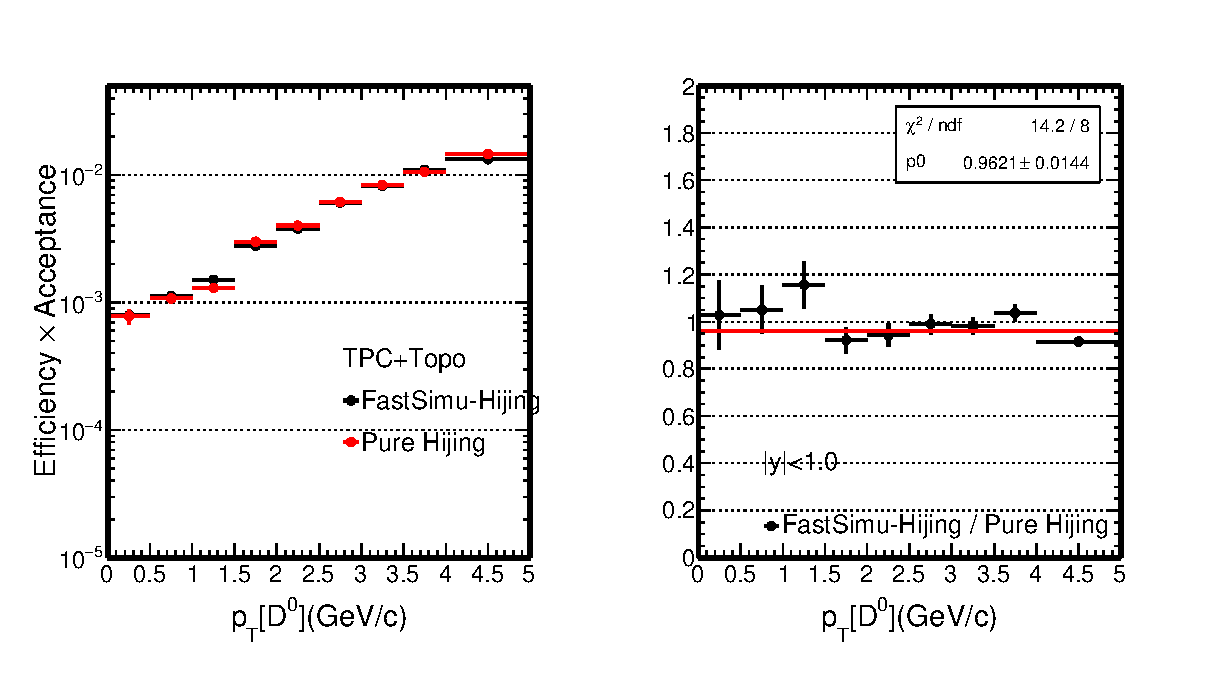
\includegraphics[keepaspectratio,width=1.0\textwidth,angle=0]{figure/Run14_D0HFT/Physics_FastHijingVsPureHijing_HFTTopo.eps}
\caption{The comparison of $D^0$ TPC + HFT match + Topological acceptance $\times$ efficiency between Hijing + GEANT (red) and Fast-Simulation with Hijing input with wide binning (black). (right) Double ratio of these acceptance to Hijing.}
\label{d0hfttopoeff2}
\end{figure}

From Hijing + GEANT simulation, we know exactly whether the HFT matched track is real match or mismatch, so we can determine the HFT real matched efficiency $\times$ acceptance for $D^0$ reconstruction from Hijing sample. Fig.~\ref{d0hfttoporealeff} shows these real matched efficiency $\times$ acceptance comparison between Hijng + GEANT and our previously Fast-Simulation. The right panel shows the double ratio of these efficiency and fitted with a line, the parameters shows $\sim$0.98 which means the (previous) Fast-Simulation can well reproduce the real HFT matched reconstruction efficiency. Fig.~\ref{d0hfttoporealeff2} shows the same plots of the comparison with different binning. 

\begin{figure}[htbp]
\centering
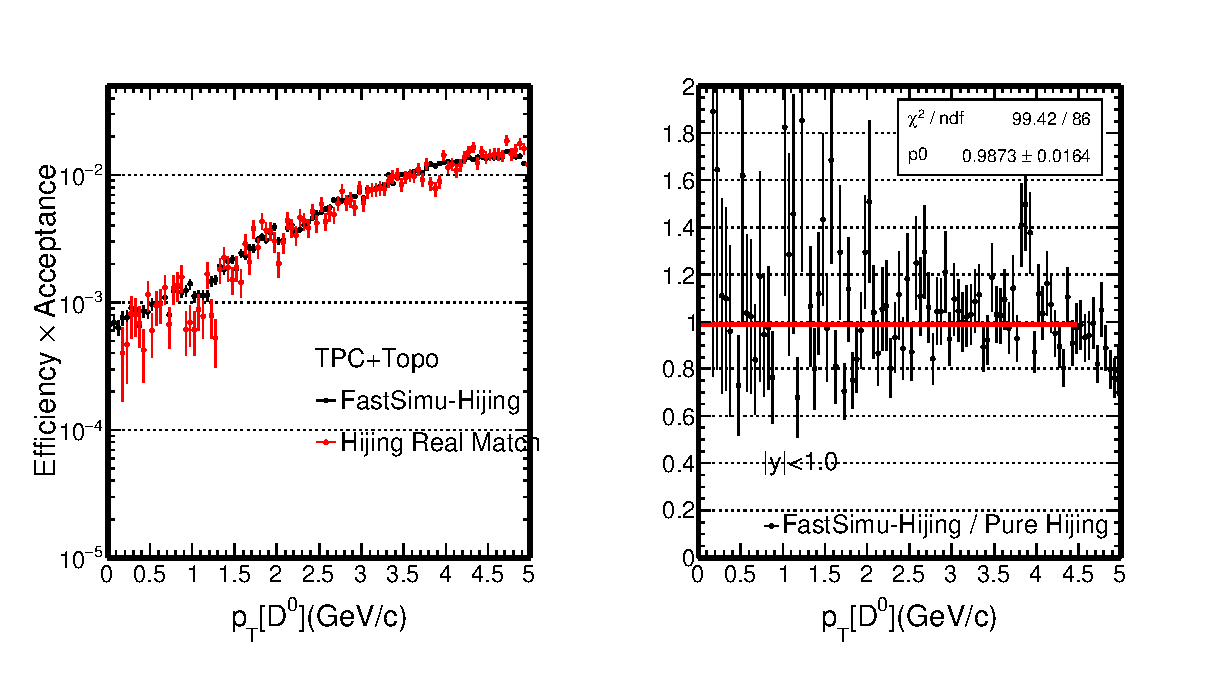
\includegraphics[keepaspectratio,width=1.0\textwidth,angle=0]{figure/Run14_D0HFT/Real_Physics_FastHijingVsPureHijing_HFTTopo2.eps}
\caption{The comparison of $D^0$ TPC + HFT Real match + Topological acceptance $\times$ efficiency between Hijing + GEANT (red) and Fast-Simulation with Hijing input (black). (right) Double ratio of these acceptance to Hijing.}
\label{d0hfttoporealeff}
\end{figure}

\begin{figure}[htbp]
\centering
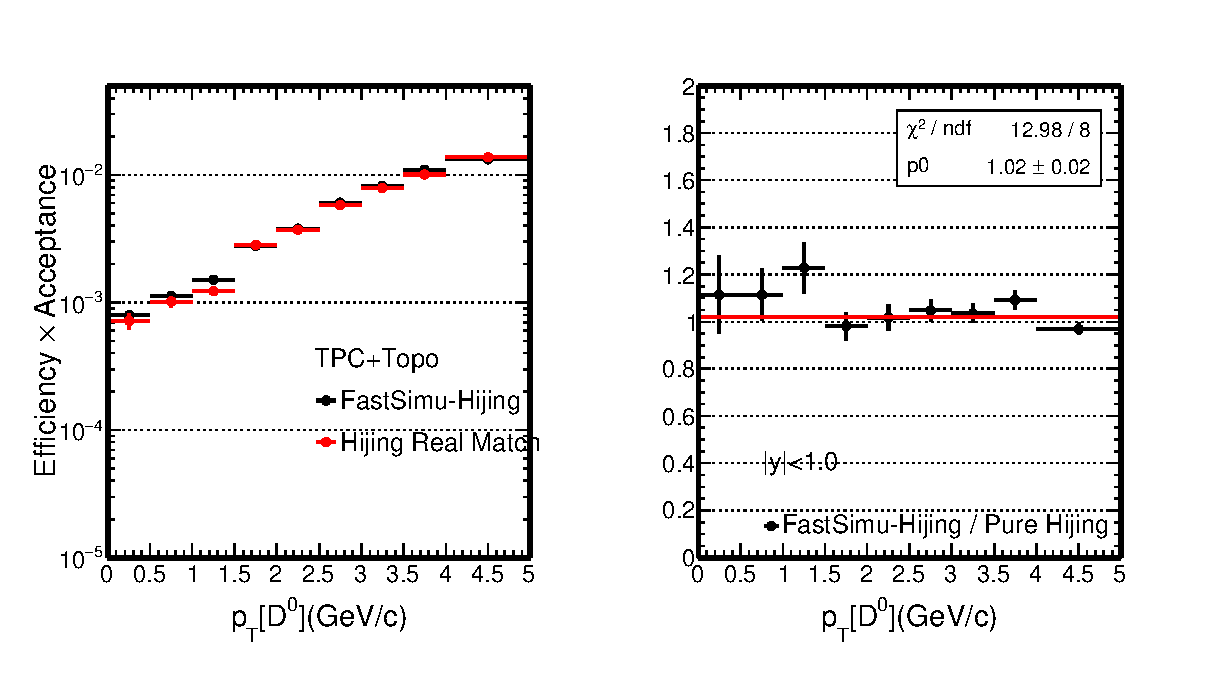
\includegraphics[keepaspectratio,width=1.0\textwidth,angle=0]{figure/Run14_D0HFT/Real_Physics_FastHijingVsPureHijing_HFTTopo.eps}
\caption{The comparison of $D^0$ TPC + HFT Real match + Topological acceptance $\times$ efficiency between Hijing + GEANT (red) and Fast-Simulation with Hijing input with wide binning (black). (right) Double ratio of these acceptance to Hijing.}
\label{d0hfttoporealeff2}
\end{figure}

If we compare with the previous Hijing HFT matched efficiency (not necessary to be real matched), it also indicate that most of the Mis-matched daughter tracks are removed by topological cuts as we said in the assumptions. Fig.~\ref{d0hfttopoAlleff} shows the different components contributions directly from Hijing, the black one is HFT matched, red one requires all the daughter tracks are real matched and the blue one shows at least one of the daughter tracks are mis-matched. Right panel shows the relative fraction of the real match and mis-mismatch contribution. As see, most of the mis-matched tracks are removed, but still there are $\sim$5\% contribution from this study.

\begin{figure}[htbp]
\centering
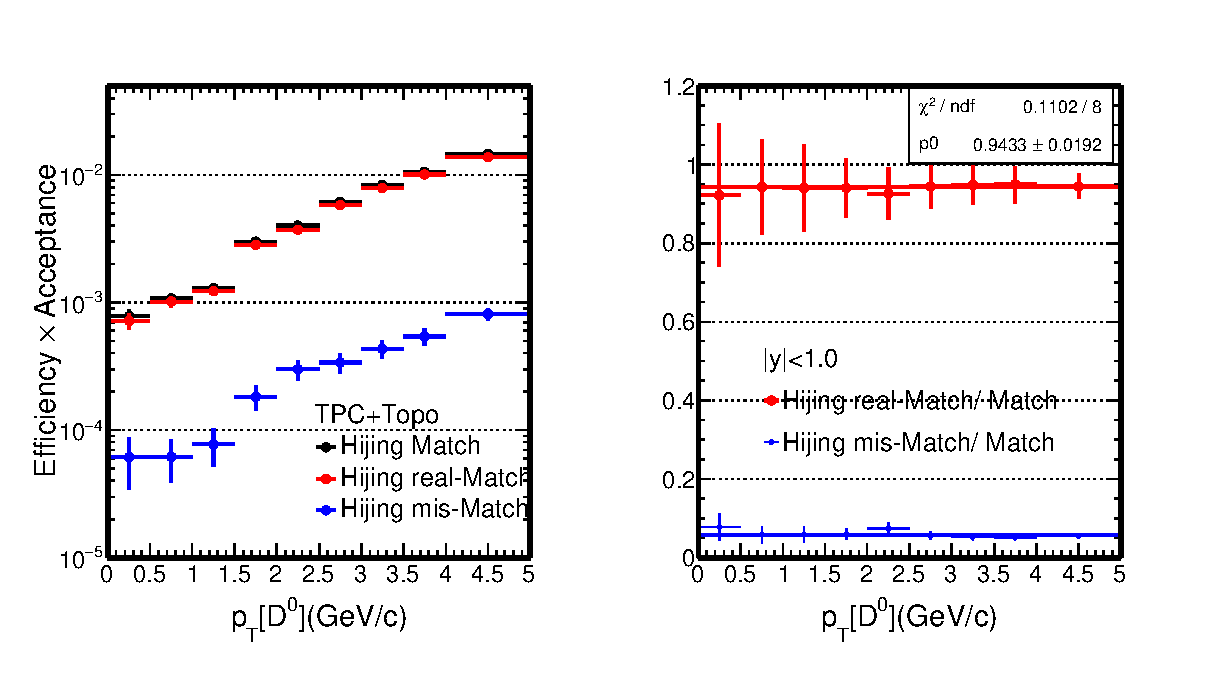
\includegraphics[keepaspectratio,width=1.0\textwidth,angle=0]{figure/Run14_D0HFT/ALL_Physics_FastHijingVsPureHijing_HFTTopo.eps}
\caption{The comparison of $D^0$ TPC + HFT (real/mis) match + Topological acceptance $\times$ efficiency for Hijing + GEANT. (right) Double ratio of the components form Hijing.}
\label{d0hfttopoAlleff}
\end{figure}

Above all the discussions in this section ~\ref{validationeff}, we are confident that the Fast-Simulation method can well reproduce the acceptance and efficiency for this HFT related analysis. The precision as shown on Fig.~\ref{d0hfttopoeff2} is good enough for our efficiency study. For the missed-match check, there are $\sim$5\% contributions in the signals. And there is another approvement that will describe in the following section.

\subsubsection{Validation Topological Distributions}
\label{validationTopo}

As discussed before, we can extract the topological variables from both Hijing + GEANT and Fast-Simulation relay on those Hijing input. Similar as we did in Sec. ~\ref{d0efficiency}, we can compare the topological distributions from these two procedures. This will be another evidence that our Fast-Simulation can well reproduce the topological variables which is crucial for these kind of secondary vertex reconstruction analysis.

\begin{figure}[htbp]
\begin{minipage}[htbp]{0.52\linewidth}
\centering
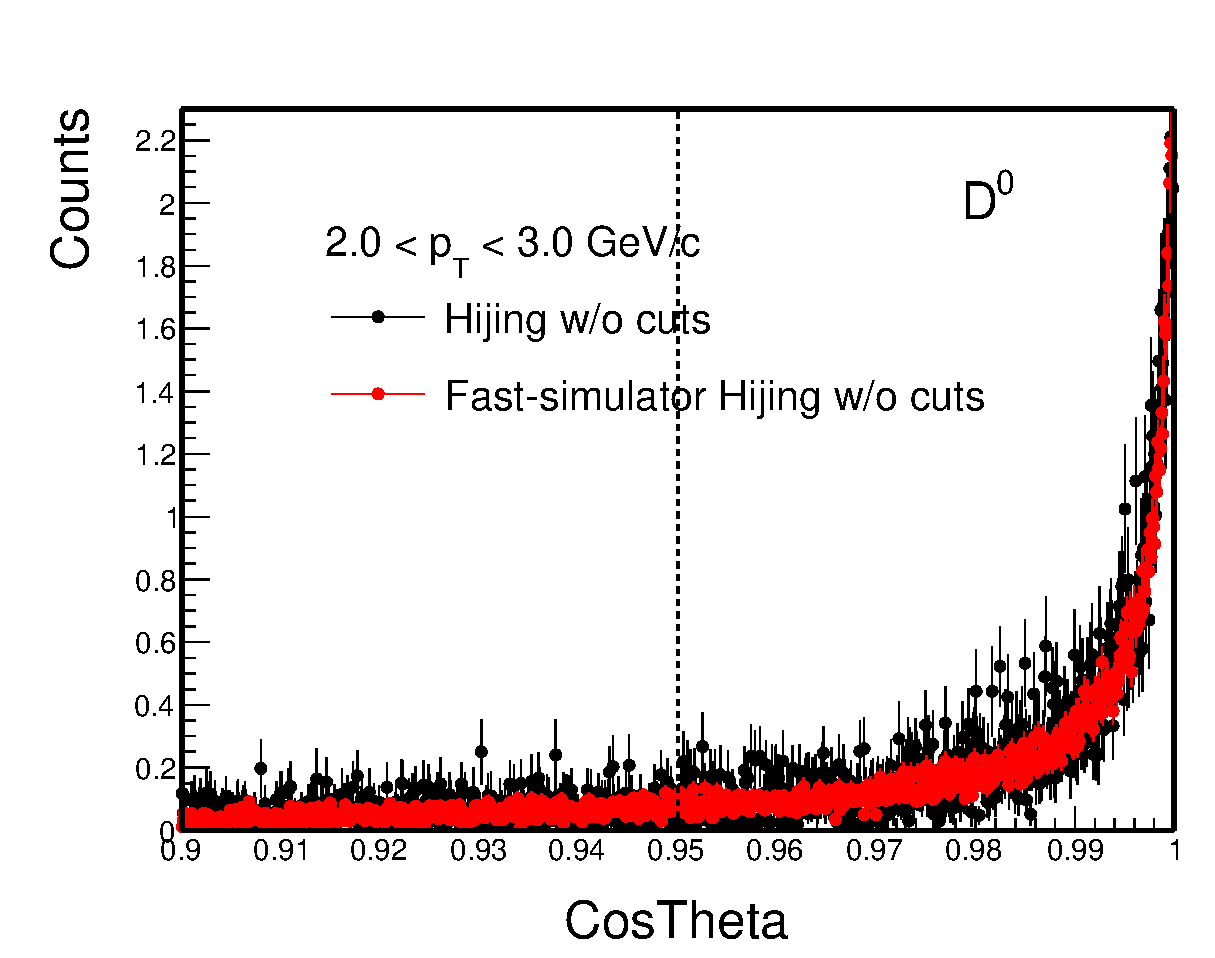
\includegraphics[width=1.0\textwidth,angle=0]{figure/Run14_D0HFT/HijingcosTheta.eps}
\caption{ $D^0$ cosTheta distribution in most central 0-10\% between Hijing and Fast-Simulation.\label{Hijingpointingangle}}
\end{minipage}
\hfill
\begin{minipage}[htbp]{0.52\linewidth}
\centering
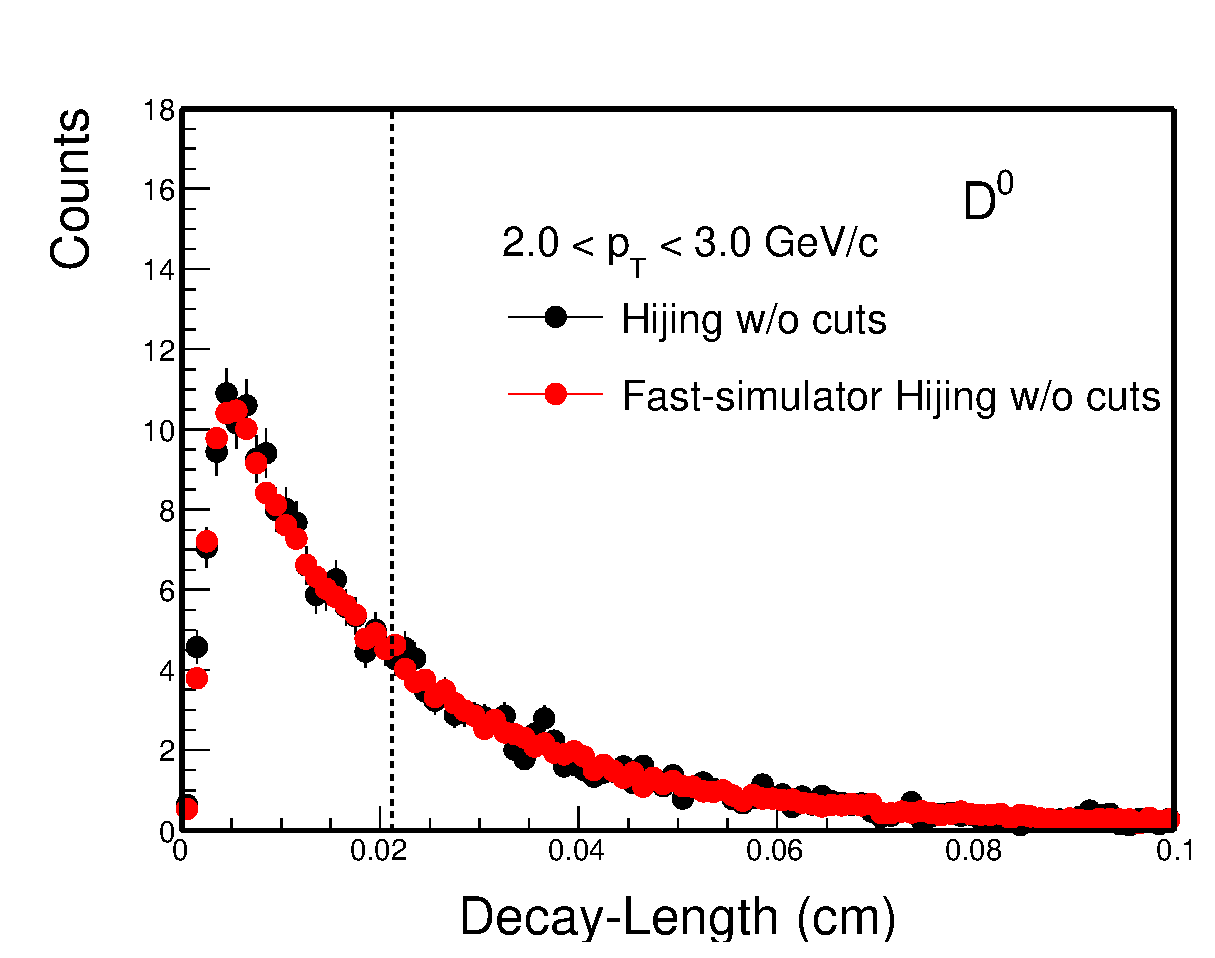
\includegraphics[width=1.0\textwidth,angle=0]{figure/Run14_D0HFT/HijingDecayL.eps} 
\caption{ $D^0$ decay length distribution in most central 0-10\% between Hijing and Fast-Simulation.\label{HijingDecayL}}
\end{minipage}
\end{figure}

\begin{figure}[htbp]
\begin{minipage}[htbp]{0.52\linewidth}
\centering
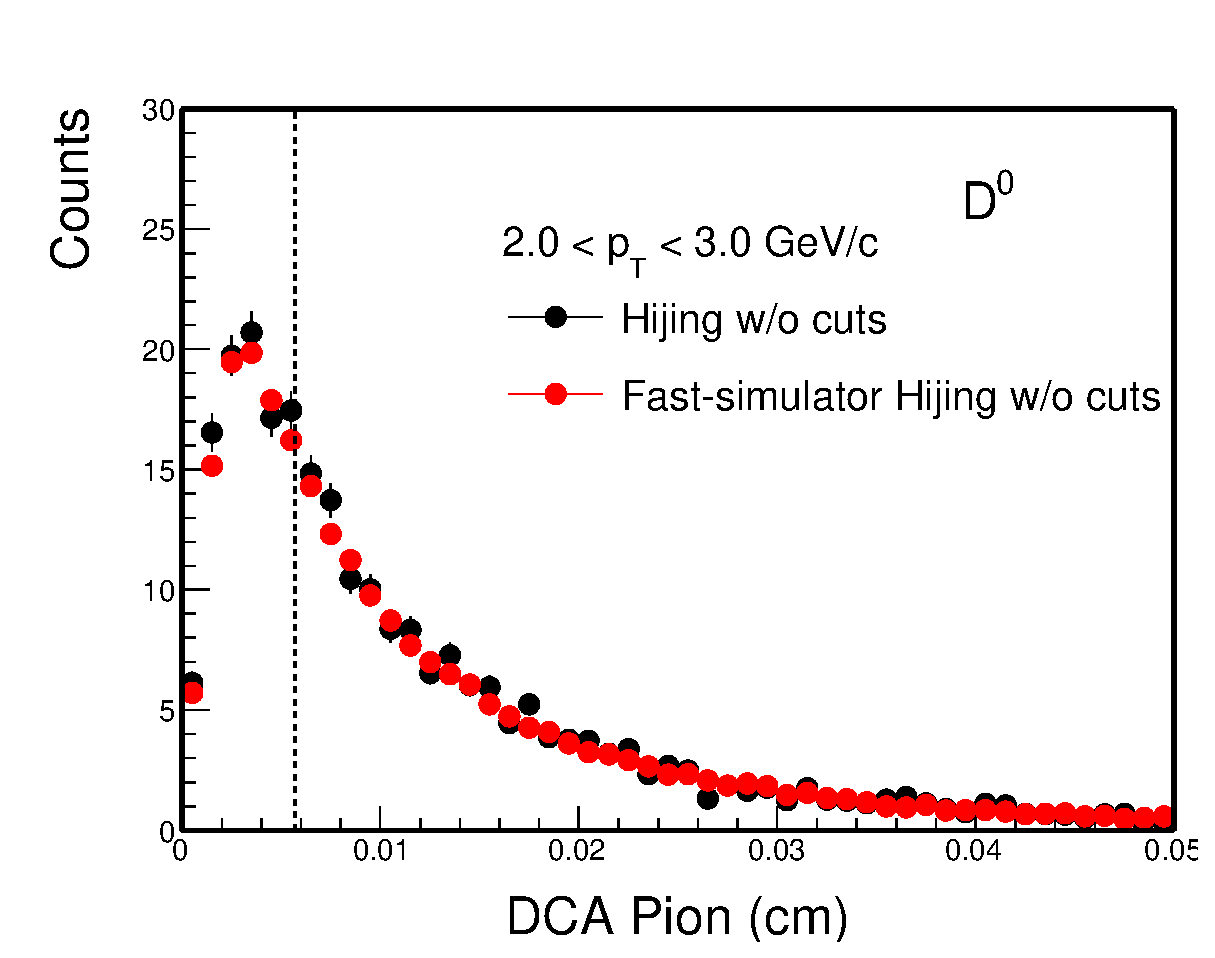
\includegraphics[width=1.0\textwidth,angle=0]{figure/Run14_D0HFT/HijingdcaPions.eps}
\caption{ $D^0$ pions Dca distribution in most central 0-10\% between Hijing and Fast-Simulation.\label{HijingdcaPions}}
\end{minipage}
\hfill
\begin{minipage}[htbp]{0.52\linewidth}
\centering
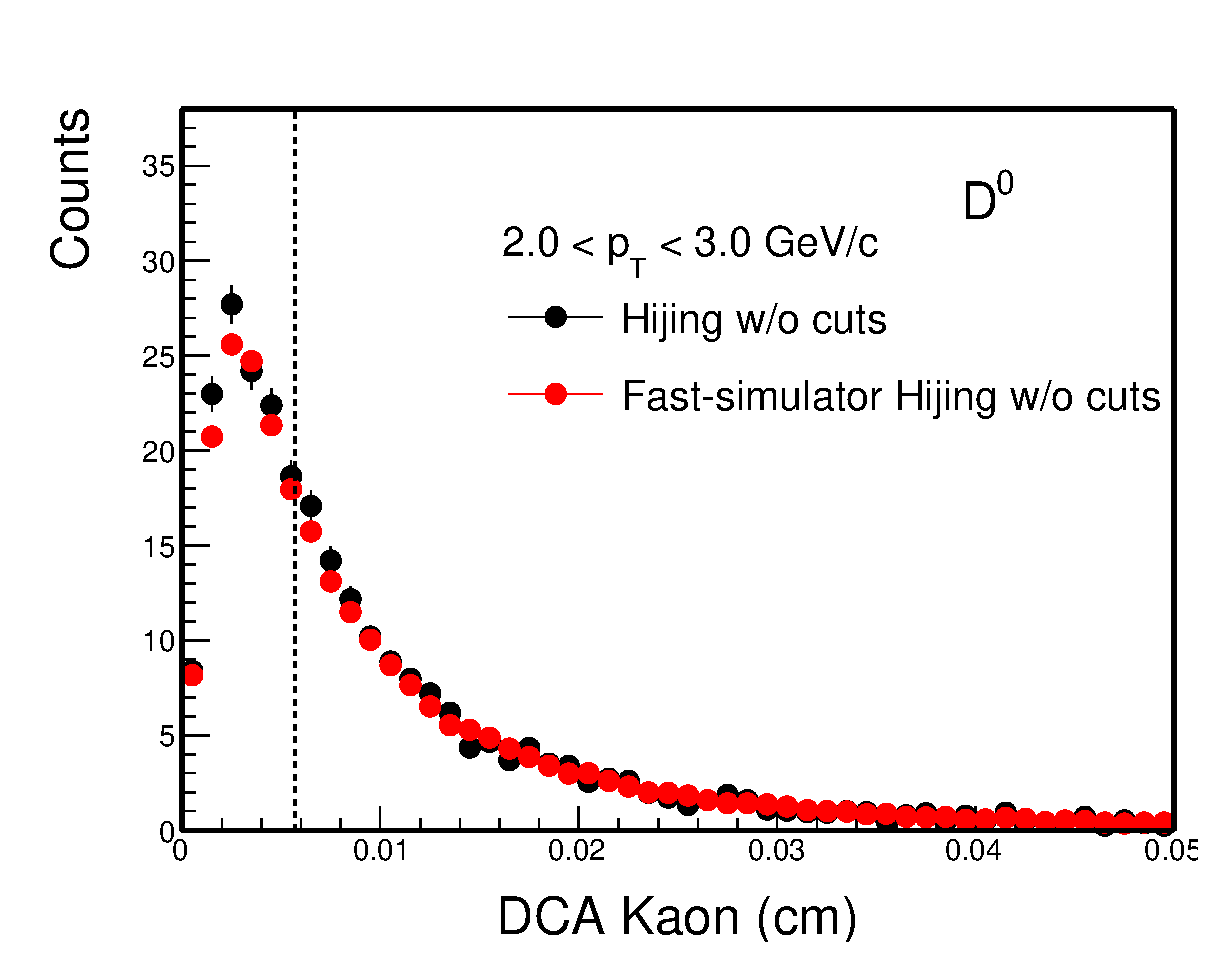
\includegraphics[width=1.0\textwidth,angle=0]{figure/Run14_D0HFT/HijingdcaKaons.eps} 
\caption{ $D^0$ kaons Dca distribution in most central 0-10\% between Hijing and Fast-Simulation.\label{HijingdcaKaons}}
\end{minipage}
\end{figure}

\begin{figure}[htbp]
\centering
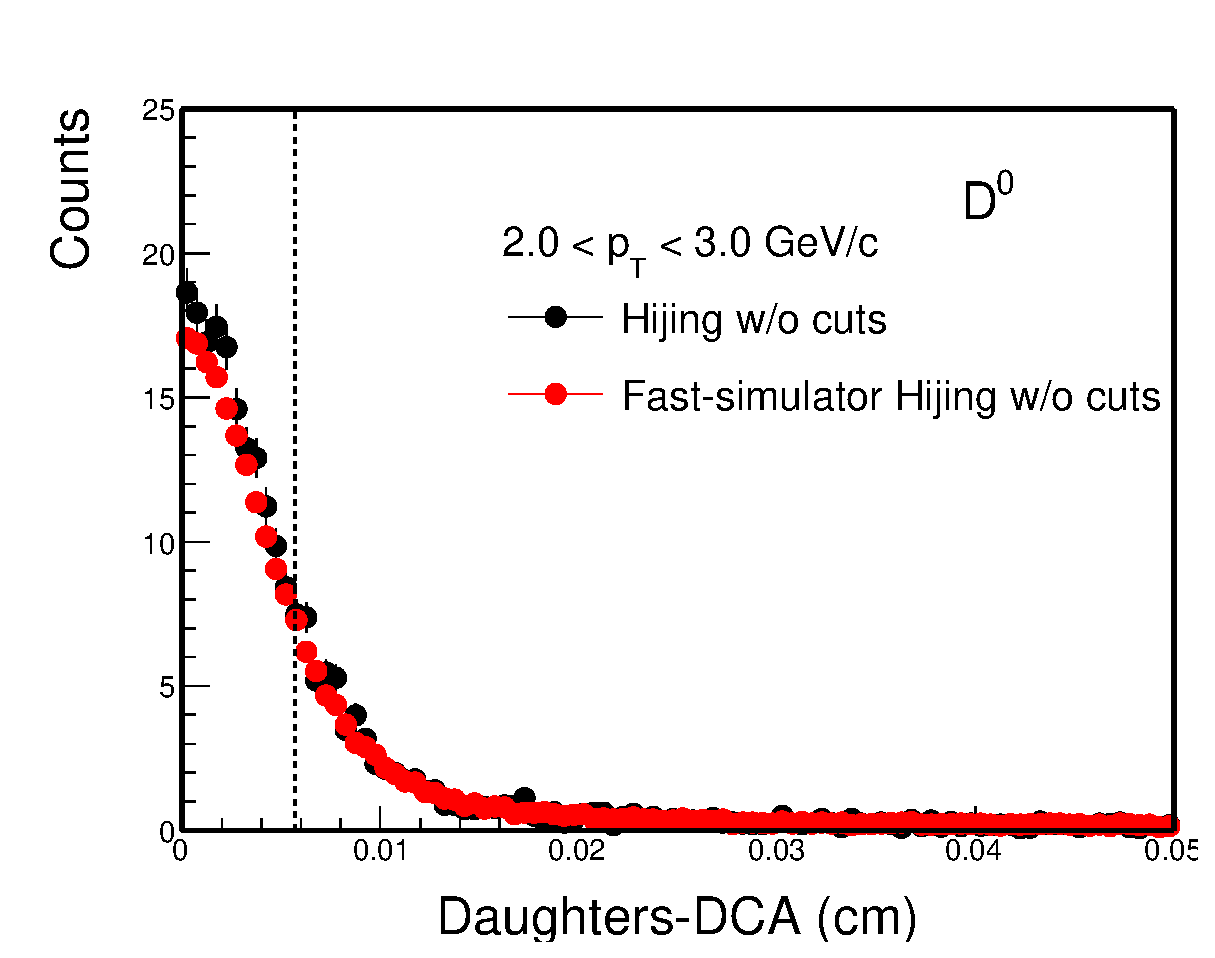
\includegraphics[keepaspectratio,width=0.52\textwidth]{figure/Run14_D0HFT/HijingdcaDaughters.eps}
\caption{$D^0$ dcaDaughters distribution in most central 0-10\% between Hijing and Fast-Simulation.}
\label{HijingdcaDaughters}
\end{figure}

From Fig.~\ref{Hijingpointingangle} to Fig.~\ref{HijingdcaDaughters}, these are the topological variables used for the $D^0$ reconstruction. The topological distributions can be extracted both directly from Hijng + GEANT and from Fast-Simulation relay on Hijing input. The Fast-Simulation part was the same package as we used for the efficiency study before.

As seen, the comparison of topological variables from Hijing have a very good agreement, which means again our Fast-Simulation method can well reproduce the topological variables in Hijing sample just as in the real data case. In another word, the efficiency estimation from this Hijing-Data-Driven Fast-Simulation is reliable.  This is the other confident as we discussed in the last part of previous section ~\ref{validationeff}.


There are two more assumptions which were not answered yet. Here we are trying to discuss a little bit in the following part.

\subsection{\label{concern1} Secondary Track Contribution}

The Fast-Simulation is validated with primary track in the procedure Fig.~\ref{validation0}. All the tracks for HFT matching ratio and Dca inputted to Fast-Simulation is primary track. Based on the Hijing sample we can study the secondary track contribution since in the real data part we can't distinguish primary track and secondary track. In Hijing simulation, we use the start vertex of that track to determine whether it's primary track or secondary track.

\begin{figure}[htbp]
\centering
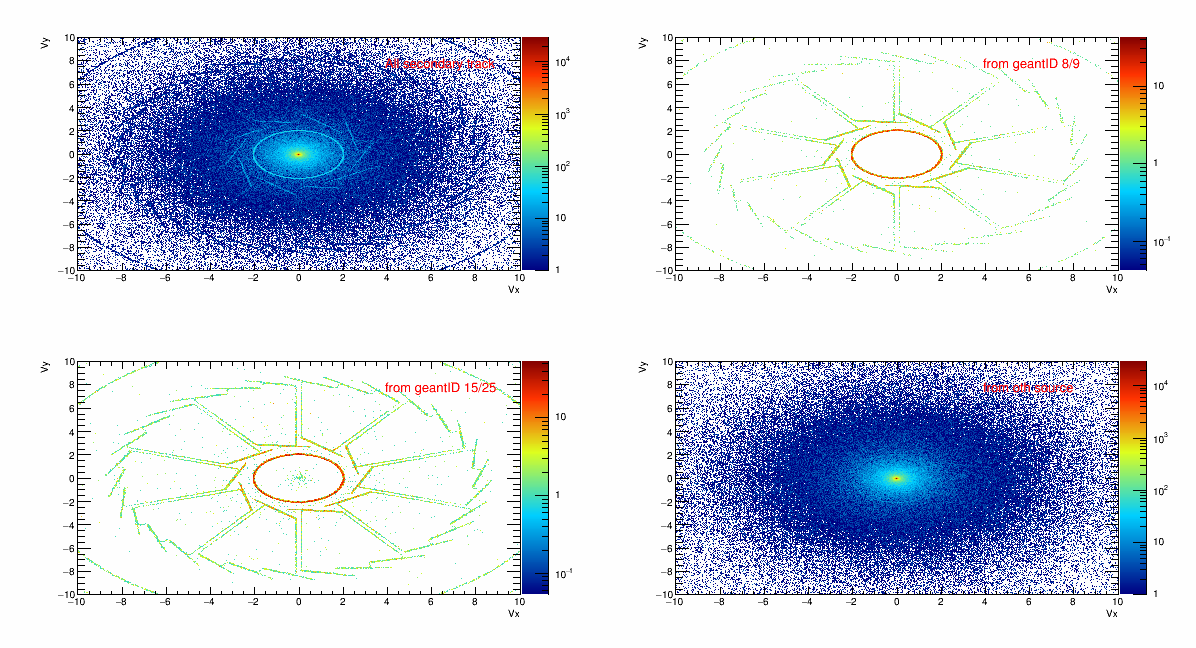
\includegraphics[keepaspectratio,width=1.0\textwidth,angle=0]{figure/Run14_D0HFT/Vtx_Pion.png}
\caption{The vertex distribution for Pions from secondary decay. Top left is the overall secondary pion tracks, top right is pion decayed from GeantID=8/9 (which is $\pi^{\pm}$), bottom left is pion decayed from GeantID=15/25 (which is anti-proton and anti-neutron), bottom right is decayed from other source such as the lambda (anti)sigma and Xi0}
\label{Vtx_Pion}
\end{figure}

\begin{figure}[htbp]
\centering
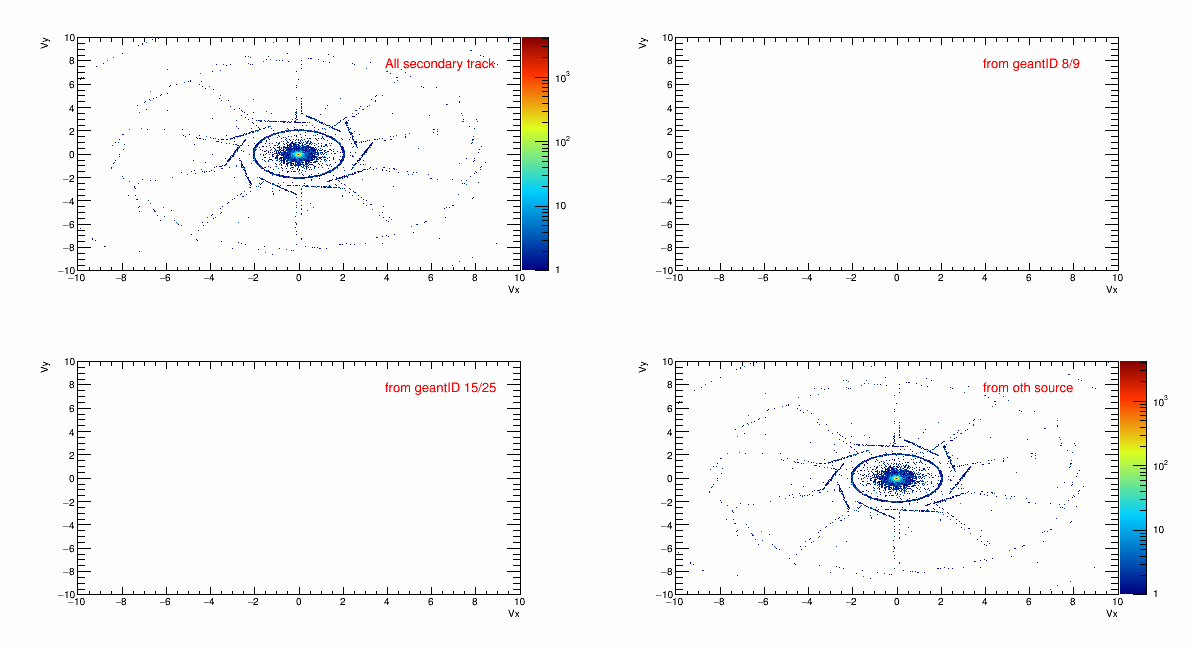
\includegraphics[keepaspectratio,width=1.0\textwidth,angle=0]{figure/Run14_D0HFT/Vtx_Kaon.png}
\caption{The vertex distribution for Kaons from secondary decay. Top left is the overall secondary pion tracks, top right is pion decayed from GeantID=8/9 (which is $\pi^{\pm}$), bottom left is pion decayed from GeantID=15/25 (which is anti-proton and anti-neutron), bottom right is decayed from other source}
\label{Vtx_Kaon}
\end{figure}


Fig.~\ref{Vtx_Pion} shows the pions vertex distributions from the secondary decay. The first one is the overall secondary pion vertex distributions and we can clearly saw some HFT structure. Top right panel is pions decayed from GeantID==8/9 (which is $\pi^{\pm}$), this part is the knocked out particles with HFT. The bottom left is pion decayed from GeantID==15/25 (which is anti-proton and anti-neutron), this is the normal annihilation particles. The last one bottom right shows the pions decayed from other source such as the lambda (anti)sigma and Xi0.

For the secondary tracks, they have different contributions to the HFT mathing ratio. The fraction of the secondary tracks contributions can be found in the Fig.~\ref{Fraction_Pion}, as see in the $p_{T}$ range around 2-3 GeV/c there is a visible contributions from the annihilation with the materials, which will final contribute to the HFT matching ratio.

\begin{figure}[htbp]
\centering
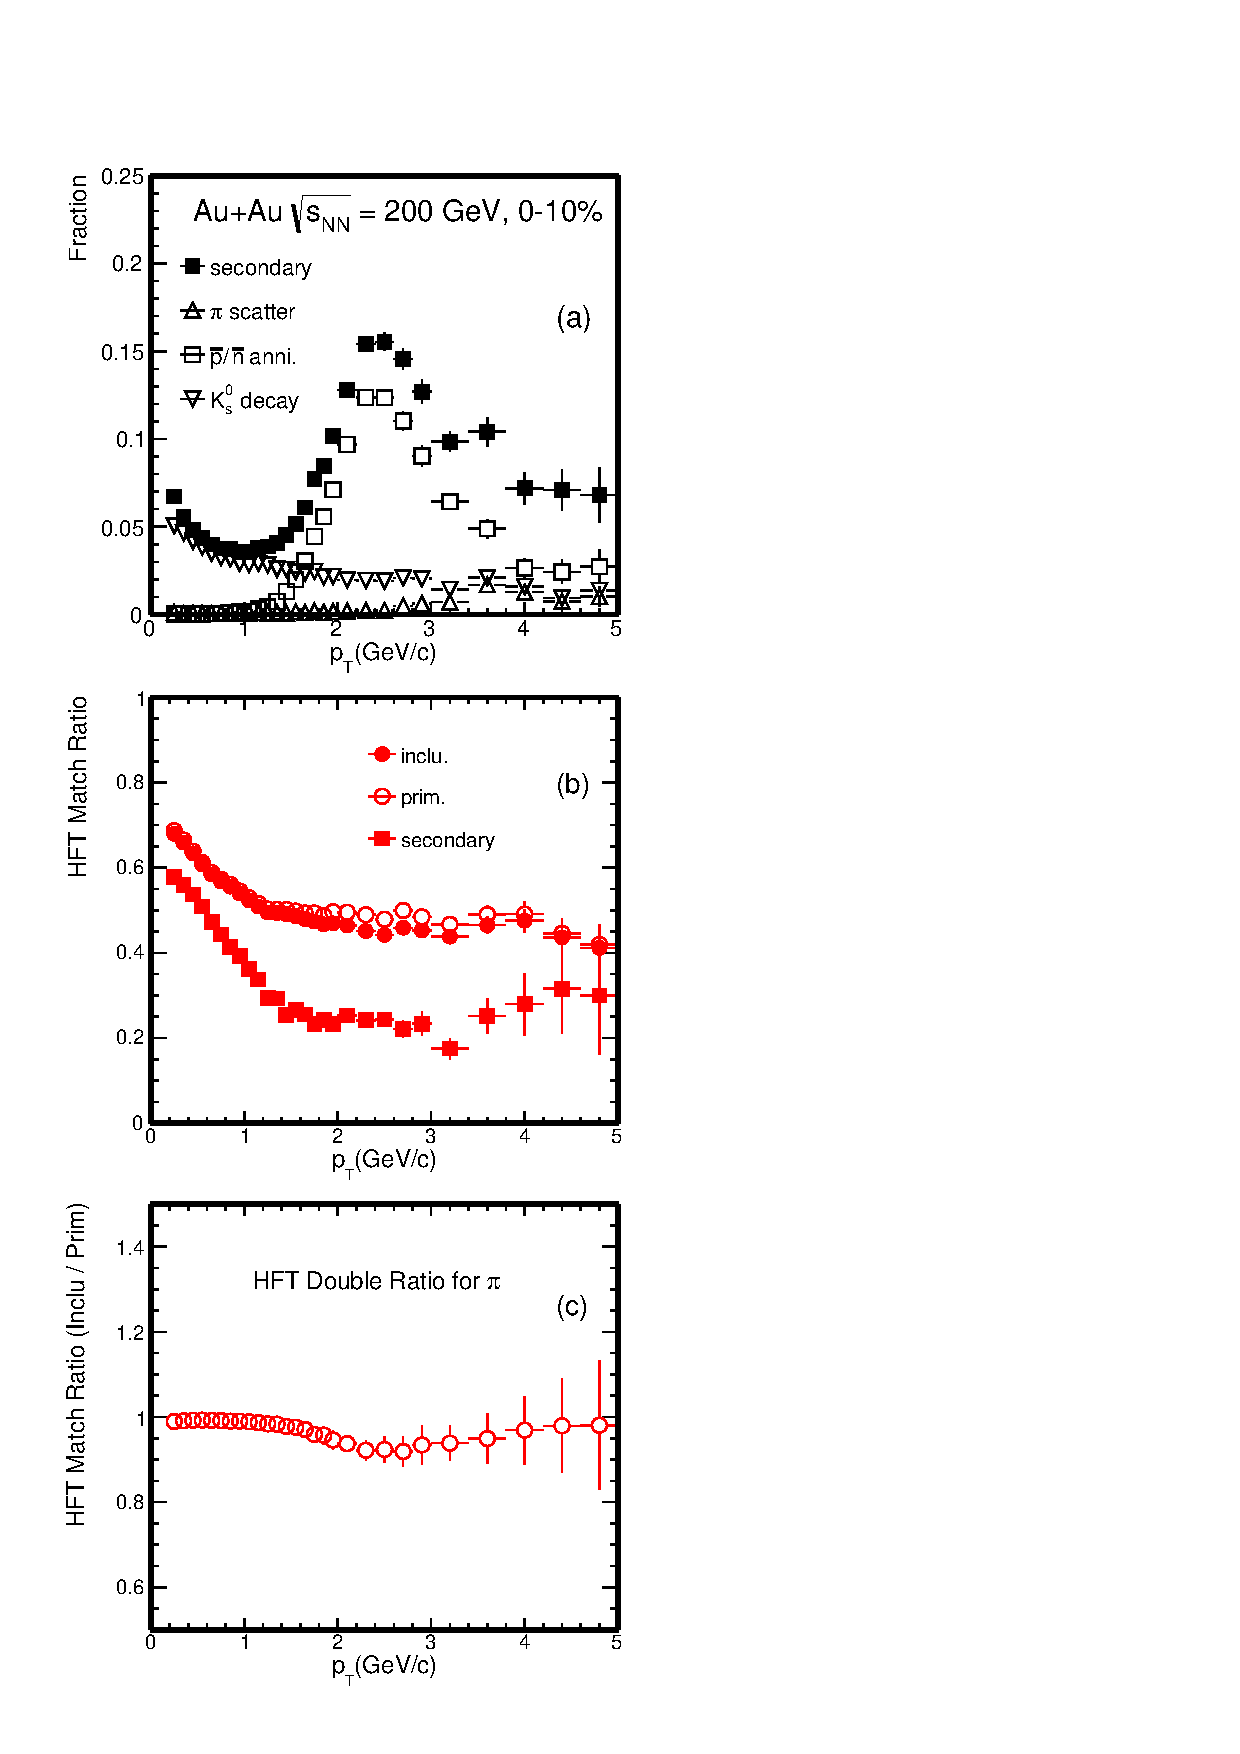
\includegraphics[keepaspectratio,width=1.0\textwidth,angle=0]{figure/Run14_D0HFT/Fraction_Pion.pdf}
\caption{The fraction of the different sources for the pion spectra, including the primary particles which is out of the range, the secondary sources include form parent GeantId =8/9, GeantId=15/25 and others source.}
\label{Fraction_Pion}
\end{figure}

\begin{figure}[htbp]
\centering
\includegraphics[keepaspectratio,width=1.0\textwidth,angle=0]{figure/Run14_D0HFT/Fraction_Kaon.pdf}
\caption{The fraction of the different sources for the kaon spectra, including the primary particles which is out of the range, the secondary sources include form parent GeantId =8/9, GeantId=15/25 and others source.}
\label{Fraction_Kaon}
\end{figure}


The secondary track have kind of different performance compare to the primary track such as the HFT match ratio shown on Fig.~\ref{HijingPionsRatio}. The solid circle is the inclusive one for HFT matching ratio, the empty circle is for the primary pions and the solid square is for the secondary pions. All these HFT match ratios are after applying exactly the same cut as real data analysis. The low match ratio for secondary track is reasonable since they are decayed far away from the vertex and most of them do not have three HFT hits. The more contribution from the secondary track, the more difference we observed between inclusive one and primary one. The bottom panel shows the HFT matching double ratio of inclusive one over primary one. For the pions, since the secondary pion have some contributions, we do saw the different between primary one ans inclusive one at some certain $p_T$ range for this HFT match ratio. For the kaons, the relative secondary contribution is small, that's why there is no big difference between primary and inclusive ones as see on Fig.~\ref{HijingKaonsRatio}. 

\begin{figure}[htbp]
\begin{minipage}[htbp]{0.47\linewidth}
\centering
\includegraphics[width=1.0\textwidth,angle=0]{figure/Run14_D0HFT/Double_Ratio_Pion.eps}
\caption{ HFT Matching Ratio for Pions, compare between primary track and secondary tracks relay on Hijing. (bottom) The double ratios of inclusive one to primary tracks.\label{HijingPionsRatio}}
\end{minipage}
\hfill
\begin{minipage}[htbp]{0.47\linewidth}
\centering
\includegraphics[width=1.0\textwidth,angle=0]{figure/Run14_D0HFT/Double_Ratio_Kaon.eps} 
\caption{ HFT Matching Ratio for Kaons, compare between primary track and secondary tracks relay on Hijing.  (bottom) The double ratios of inclusive one to primary tracks.\label{HijingKaonsRatio}}
\end{minipage}
\end{figure}


\begin{figure}[htbp]
\centering
\includegraphics[keepaspectratio,width=1.0\textwidth,angle=0]{figure/Run14_D0HFT/Physics_FastHijingVsPureHijing_HFTTopo_inclusive.pdf}
\caption{The comparison of $D^0$ TPC + HFT match + Topological acceptance $\times$ efficiency between Hijing + GEANT (red) and Fast-Simulation with Hijing input (black) from the inclusive particles. (right) Double ratio of these acceptance to Hijing.}
\label{d0hfttoporealeffinclusive}
\end{figure}

\begin{figure}[htbp]
\centering
\includegraphics[keepaspectratio,width=1.0\textwidth,angle=0]{figure/Run14_D0HFT/Physics_FastHijingVsPureHijing_HFTTopo_inclusiveCorrect.pdf}
\caption{The comparison of $D^0$ TPC + HFT match + Topological acceptance $\times$ efficiency between Hijing + GEANT (red) and Fast-Simulation with Hijing input (black) from the inclusive particles after the correction from secondary particles. (right) Double ratio of these acceptance to Hijing.}
\label{d0hfttoporealeffinclusivecorrect}
\end{figure}


This secondary track contribution for our efficiency correction need to be taken care, especially for Pions. There are a few percent contributions from our Hjing simulation study. In our real data efficiency correction, we took this double ratio from Hijing as an additional correction factor for the HFT matching ratio, since the data part can only obtained the inclusive one. After this additional correction, we still be able to obtain the precision like Fig.~\ref{d0hfttopoeff2}.

For the secondary track Dca contributions, we tested with the inclusive track Dca or primary track Dca. In principle, with the inclusive tracks, they should have slightly broader distributions. But in our test, it seems that these contributions to the final $D^0$ efficiency is really small. This maybe due to the limited Hijing statistics or the slightly Dca difference does not contribute much. But in our real data case, we do not take this secondary Dca contributions as additional correction factor yet.


\subsection{Vertex Resolution Contribution}
\label{concern2}

As discussed before, the vertex resolution in peripheral events still have some contributions. If those peripheral events vertices are out of hundreds or dozens of $\upmu$ m vertex resolution, they are not likely to contribute to the D mesons foreground (maybe not even the background). To correctly count the number of peripheral events we need to understand the vertex resolution. The 2D $\textup{Dca}_{\textup{XY}}$ $\textup{Dca}_\textup{Z}$ distributions are the only input to the Fast-Simulation for this effect. They contain both the vertices and tracks contribution. 

Fig.~\ref{vtxX_vsCent} shows the vertex resolution in the X direction using the sub-event method. We divide the event to two randomly subevent, and then reconstruct two vertexes. The difference of the two vertexes can be somehow demonstrate the vertex resolutions.

\begin{figure}[htbp]
\begin{minipage}[htbp]{0.47\linewidth}
\centering
\includegraphics[width=1.0\textwidth,angle=0]{figure/Run14_D0HFT/vxtX_70_80.png}
\caption{ FWHM of the subEvent vertex resolutions for 70-80\%.\label{vtxX_70_80}}
\end{minipage}
\hfill
\begin{minipage}[htbp]{0.47\linewidth}
\centering
\includegraphics[width=1.0\textwidth,angle=0]{figure/Run14_D0HFT/vtxX_20_30.png} 
\caption{ FWHM of the subEvent vertex resolutions for 20-30\%.\label{vtxX_20_30}}
\end{minipage}
\end{figure}

\begin{figure}
\centering
\includegraphics[width=0.6\textwidth]{figure/Run14_D0HFT/vtxX_vsCent.pdf}
\caption{ Full Width of the Half Maximum (FWHM ) for Vertex resolution using sub-event method versus centralities in Au + Au collisions.}
\label{fig:vtxX_vsCent} 
\end{figure}

To solve this problem, we need to unfold the vertex resolution from 2D Dca distributions, and this is not straightforward since the vertex resolution contribution could be in the same order of the Dca resolution and this is not reliable (subtracting two numbers that are close to each other have very large uncertainties). There is another way we can relay on to obtain this correction factor, which is the Minimum Bias Hjing simulation sample. From Hijing sample we know the true efficiency for any centrality species, and from the Fast-Simulation we can obtain the efficiency including those vertex effect. The difference can be took as the additional correction factor for real data analysis if this effect is not too big. The MB Hijing sample we used here is from the same setup as we discussed before, and the only difference compared to the 0-10\% Hjing sample is the impact parameters (b). But for our centrality selection, we still use grefumlt for both data and simulation.

For the QA of the simulation samples, including HFT matching ratio and Dca resolutions for different centralities, all the details can be found in the next links:

\url{http://portal.nersc.gov/project/star/xlchen/D0_Hijing/QA/all/}

\begin{figure}[htbp]
\begin{minipage}[htbp]{0.47\linewidth}
\centering
\includegraphics[width=1.0\textwidth,angle=0]{figure/Run14_D0HFT/70_80_0.pdf}
\caption{ The comparison of $D^0$ acceptance between Hijing + GEANT (black) and Fast-Simulation with Hijing input (red). (bottom) Double ratio of these acceptance of Hijing to Fast-Simulation.\label{70_80_0}}
\end{minipage}
\hfill
\begin{minipage}[htbp]{0.47\linewidth}
\centering
\includegraphics[width=1.0\textwidth,angle=0]{figure/Run14_D0HFT/70_80_1.pdf} 
\caption{ The comparison of $D^0$ TPC acceptance $\times$ efficiency between Hijing + GEANT (black) and Fast-Simulation with Hijing input (red). (bottom) Double ratio of these efficiency of Hijing to Fast-Simulation.\label{70_80_1}}
\end{minipage}
\end{figure}

\begin{figure}[htbp]
\begin{minipage}[htbp]{0.47\linewidth}
\centering
\includegraphics[width=1.0\textwidth,angle=0]{figure/Run14_D0HFT/70_80_2.pdf}
\caption{ The comparison of $D^0$ TPC + HFT match acceptance $\times$ efficiency between Hijing + GEANT (black) and Fast-Simulation with Hijing input (red). (bottom) Double ratio of these acceptance of Hijing to Fast-Simulation.\label{70_80_2}}
\end{minipage}
\hfill
\begin{minipage}[htbp]{0.47\linewidth}
\centering
\includegraphics[width=1.0\textwidth,angle=0]{figure/Run14_D0HFT/70_80.pdf} 
\caption{ The comparison of $D^0$ TPC + HFT match + Topological acceptance $\times$ efficiency between Hijing + GEANT (black) and Fast-Simulation with Hijing input (red). (bottom) Double ratio of these efficiency of Hijing to Fast-Simulation.\label{70_80_3}}
\end{minipage}
\end{figure}

The first vertex contribution we checked is for the centrality species 70-80\%. Follow the same procedures as we discussed for 0-10\%, we did the validation step by step. First is the acceptance check as shown on Fig.~\ref{70_80_0}, the results from Hijing and Fast-Simulation matched very well for this most peripheral events, which is the same as our expection. The second step is check the kinematic with the reconstructed TPC tracking information. These was involved with the TPC tracking efficiency lost and the momentum resolution. the result in Fig.~\ref{70_80_1} shows good agreement.

The next step for this peripheral centrality will be fold in the HFT matching efficiency and the results shown in Fig.~\ref{70_80_2}. As see, the two curves are close with each other and the double ratio was close to unity. The last step will be the topological contributions which also including the vertex contributions. Fig.~\ref{70_80_3} shows this efficiency $\times$ Acceptance comparison between Hijing and Fast-Simulation after the TPC, HFT matching and topological cuts for the 70-80\% centralities. As see, due to the involved vertex resolution contribution for this peripheral events, the agreement between Hijing and Fast-Simulation was not good anymore. If we try to fit the double ratio shown in the lower panel, the difference can be as large as a factor of $\sim$1/0.29.


\begin{figure}[htbp]
\begin{minipage}[htbp]{0.47\linewidth}
\centering
\includegraphics[width=1.0\textwidth,angle=0]{figure/Run14_D0HFT/70_80.pdf}
\caption{ The comparison of $D^0$ TPC + HFT match + Topological between Hijing (black) and Fast-Simulation for 70-80\% centrality (red). (bottom) Double ratio to Fast-Simulation.\label{70_80}}
\end{minipage}
\hfill
\begin{minipage}[htbp]{0.47\linewidth}
\centering
\includegraphics[width=1.0\textwidth,angle=0]{figure/Run14_D0HFT/60_70.pdf} 
\caption{ The comparison of $D^0$ TPC + HFT match + Topological between Hijing (black) and Fast-Simulation for 60-70\% centrality (red). (bottom) Double ratio to Fast-Simulation.\label{60_70}}
\end{minipage}
\end{figure}

\begin{figure}[htbp]
\begin{minipage}[htbp]{0.47\linewidth}
\centering
\includegraphics[width=1.0\textwidth,angle=0]{figure/Run14_D0HFT/50_60.pdf}
\caption{ The comparison of $D^0$ TPC + HFT match + Topological between Hijing (black) and Fast-Simulation for 50-60\% centrality (red). (bottom) Double ratio to Fast-Simulation.\label{50_60}}
\end{minipage}
\hfill
\begin{minipage}[htbp]{0.47\linewidth}
\centering
\includegraphics[width=1.0\textwidth,angle=0]{figure/Run14_D0HFT/40_50.pdf} 
\caption{ The comparison of $D^0$ TPC + HFT match + Topological between Hijing (black) and Fast-Simulation for 40-50\% centrality (red). (bottom) Double ratio to Fast-Simulation.\label{40_50}}
\end{minipage}
\end{figure}

\begin{figure}[htbp]
\begin{minipage}[htbp]{0.47\linewidth}
\centering
\includegraphics[width=1.0\textwidth,angle=0]{figure/Run14_D0HFT/30_40.pdf}
\caption{ The comparison of $D^0$ TPC + HFT match + Topological between Hijing (black) and Fast-Simulation for 30-40\% centrality (red). (bottom) Double ratio to Fast-Simulation.\label{30_40}}
\end{minipage}
\hfill
\begin{minipage}[htbp]{0.47\linewidth}
\centering
\includegraphics[width=1.0\textwidth,angle=0]{figure/Run14_D0HFT/20_30.pdf} 
\caption{ The comparison of $D^0$ TPC + HFT match + Topological between Hijing (black) and Fast-Simulation for 20-30\% centrality (red). (bottom) Double ratio to Fast-Simulation.\label{20_30}}
\end{minipage}
\end{figure}

\begin{figure}
\centering{
\includegraphics[width=0.6\columnwidth]{figure/Run14_D0HFT/Mcd0Eff_20_80_vsCent.pdf}
\caption{ The correction factor between Hijing and Fast-Simulation for difference centralities in tho pT ranges.}
\label{Mcd0Eff_20_80_vsCent}}
\end{figure}

For this vertex contributions, we use these double ratios as our additional correction factor for the final results. As we saw and discussed before, the most central events will not suffer this vertex contribution, but only the most peripheral and mid-peripheral events need to consider this effect. The following plots show these correction factor for different centrality species from the most peripheral to most central events.


Fig.~\ref{70_80} and the following figures show the comparison between Hijing and Fast-Simulation from different centralities, in each bottom panel, the fitted results show the expected trend. For the most peripheral events the correction factor is as large as $\sim$1/0.29 for centrality 70-80\%, $\sim$1/0.55 for centrality 60-70\%, $\sim$1/0.77 for 50-60\%, $\sim$1/0.89 for 40-50\% and $\sim$1/0.93 for 30-40\%. For the mid central, $20-30\%$ centrality, the correction effect is already small, the double ratio is close to 1. $ $

% lsjlfjalfjlajflajfkajlfjlsagdkaslkgdj  alsfjlsjfl  lajfljsl f alsjflasjfl  alfjlajsflja aljlajlfjtlejfl  aljlaw  alwjp  bcb skafk mbckaj  akhdkw
note here,

For the most central collisions, the correction factor can be neglect. This was validated and confirmed by our Hijing samples.
\subsection{Double Counting Correction} 

% \subsubsection{double counting ... To Be Added ...}

% The PID efficiency part includes the efficiency from $dE/dx$ or $n\sigma$ cut efficiency and the TOF matching+$1/\beta$ cut efficiency. The $dE/dx$ and $1/\beta$ calibration usually uses a specific set of tracks. The performance for identified particles that pass our analysis cut may not necessarily be exactly normal Gaussian distributions with means=0 and widths=1. It is desired to calibrate each individual distributions for identified particles for efficiency correction and mis-PID effect study.

% For $n\sigma$ calibration, we followed the same method as described in Ref.~\cite{Xu:2008th} to calibrate high $p_{\rm T}$ pions and protons by selecting daughters from $K_{S}^0$ and $\Lambda$ decays.

%  ... To Be Added ...

$D^0$ candidates are reconstructed with pairing $K^-$ and $\pi^+$ candidate tracks. When $D^0$ daugther $K^-$ is misidentified as a $\pi^-$ while the other daughter $\pi^+$ is misidentified as a $K^+$, the resulting pair $K^+\pi^-$ will enter into the distribution for reconstructing $\overline{D^0}$. Although the mass assignments are wrong, the pair $K^+\pi^-$ invariant mass will be still peak around the $D^0$ region with typically a broader distribution compared to the real signal. When counting the final $D^0$ candidates, these within the mass selection window will be counted twice. (See also study in previous STAR open charm hadron measurements - STAR notes below).

\url{https://drupal.star.bnl.gov/STAR/starnotes/private/psn0594}

\url{https://drupal.star.bnl.gov/STAR/starnotes/private/psn0550}

The double counting issue will certainly affect the obtained $D^0$ raw yields. In the $v_2$ analysis, since the doubly counted candidates are still coming from $D^0$, this issue should not affect the obtained central value of $v_2$. However, the statistical errors could be slightly off. For the spectra analysis, we need to consider this effect.

The double counting probability estimation need a precise determination of the PID variable distributions, $n\sigma_X$ from $dE/dx$ and $1/\beta$ from TOF. For $dE/dx$ calculation, we tried two methods

1) Select pure pion and proton samples from weak decays ($K^{S}$, $\Lambda$)

2) Look at the single particle distributions directly and perform multi-component fit in the region where the $dE/dx$ bands can be separated out.

Figure~\ref{NSigmaSummary} summarized the extracted $n\sigma_{X}$ mean values vs. $\beta\gamma$ for both methods discussed above. It looks good that in the overlapping region between different particles and different methods, the results look consistent. The dashed blue lines are parametrized function fits to the data points. These will be used to estimated the mis-identification probability.

\begin{figure}
\centering{
\includegraphics[width=0.8\columnwidth]{figure/Run14_D0HFT/NSigma_Summary_Cen_0.eps}
\caption{Top 0-10\% central Au+Au collisions: extracted $n\sigma_{X}$ mean values vs. $\beta\gamma$ for both methods discussed in the text.}
\label{NSigmaSummary}}
\end{figure}

The PID of $D^0$ daughters also involves the TOF detector. We also estimated the TOF PID variable $1/\beta$ distributions and TOF matching/PID efficiency. Figure~\ref{BetaSingle} shows the fit results on the mean and width values for $1/\beta-1/\beta_{expected}$ distributions vs. particle momentum for different particles. Similar as $dE/dx$, results in the region beyond the TOF PID are not reliable. We use results which are safe in PID for later analysis, which are $p<1.5$ GeV/$c$ for pions, $p<1$ GeV/$c$ and kaons and $p<2$ GeV/$c$ for protons. It is good to see the mean and width values are quite stable in a broad momentum region. At very low momentum, the multiple scattering effect will increase momentum resolution and $1/\beta-1/\beta_{expected}$ spread, and track energy loss will also shift the mean of $1/\beta-1/\beta_{expected}$ away from 0. But these will not affect the study here since tracks with $p_T < $ 0.6 GeV/c are not used for $D^0$ reconstruction. 

\begin{figure}
\centering{
\includegraphics[width=0.6\columnwidth]{figure/Run14_D0HFT/BetaSingle_MeanSigma_Cen_0.eps}
\caption{Top 0-10\% central Au+Au collisions: extracted $1/\beta-1/\beta_{expected}$ mean and width values vs. particle momentum for pions, kaons and protons. Results for pions and kaons at $p>1.5$ GeV/$c$ are beyond the TOF PID capability. The fit results are not reliable.}\label{BetaSingle}}
\end{figure}

With all these at hand, we can evaluate the PID efficiency. The advantage of using TOF only when available is to keep the highest efficiency as one sees from the plot. The mis-identification probability for pion and kaon daughters can be also evaluated, as shown in Figure~\ref{MisPIDPiK}. 

\begin{figure}
\centering{
\includegraphics[width=0.6\columnwidth]{figure/Run14_D0HFT/Mis_PID_PiK.eps}
\caption{Particle misidentification probability for kaons (red) and pions (black) from different centrality bins in Au+Au collisions.}\label{MisPIDPiK}}
\end{figure}

With the misidentification probability, we can reconstruct the invariant mass distributions from doubly mis-PID. The momentum resolution for pion and kaon tracks are chosen to fit to the $D^{0}$ signal peak. Figure~\ref{MisPIDMass_1} and Figure~\ref{MisPIDMass_2} show these distributions compared to the signal distributions in different $D^0$ $p_{T}$ regions. The distributions are normalized to the input real $D^{0}$ signals.

\begin{figure}
\centering{
\includegraphics[width=0.98\columnwidth]{figure/Run14_D0HFT/MassComp_MisPID_1.pdf}
\caption{Reconstructed $K\pi$ invariant mass distributions from clean PID and doubly mis-identification. The relative magnitude is fixed according to the realistic mis-identification probability. From top left to bottom right shows the distributions in $p_{T}$ bins 0-0.1 GeV/$c$, 0.1-0.2 GeV/$c$, ..., 1.9-2.0 GeV/$c$.}\label{MisPIDMass_1}}
\end{figure}

\begin{figure}
\centering{
\includegraphics[width=0.98\columnwidth]{figure/Run14_D0HFT/MassComp_MisPID_2.pdf}
\caption{Reconstructed $K\pi$ invariant mass distributions from clean PID and doubly mis-identification. The relative magnitude is fixed according to the realistic mis-identification probability. From top left to bottom right shows the distributions in $p_{T}$ bins 4-4.1 GeV/$c$, 4.1-4.2 GeV/$c$, ..., 5.9-6.0 GeV/$c$.}\label{MisPIDMass_2}}
\end{figure}

Figure~\ref{DoubleCountingSB} shows the final estimated double-counting contribution to the real signal with two different calculation methods. The black symbols show the result from directly counting the entries within 2.5$\sigma$ of the $D^0$ mass window. In real data analysis, we used the side-band distributions to normalize our fit or estimate our background. The blue data points show the result by subtracting also the side-band distributions with the same mass window selection as in event plane method $v_2$ calculation. 

\begin{figure}
\centering{
\includegraphics[width=0.6\columnwidth]{figure/Run14_D0HFT/DoubleCounting_SB.eps}
\caption{Estimated doubly-counted $D^0$ fraction to the real signal with two calculation methods from different centrality bins in Au+Au 200 GeV collisions.}\label{DoubleCountingSB}}
\end{figure}

% In the $v_2$ analysis, the doubly counted candidates are still coming from $D^0$, and there is no reason that the double counting ratio is different at different $\phi$ relative to the harmonic plane of the event. Thus the double counting issue should not affect the obtained central value of $v_2$. However, the statistical errors could be slightly off, because the 2 counts are not independent but are treated as independent when calculating $v_2$ statistic errors.

% Assuming there is no combinatorial backgroud. Let's define the $D^0$ signal yield as $S$, and that a portion $P_{SS}$ of signal has a double mis-PID count in the signal region, and a portion $P_{SB}$ of signal has a double mis-PID count in the side band region. Then the measured $D^0$ yield will be $S(1+P_{SS}-({\Delta}m_S/{\Delta}m_B)P_{SB})=S(1+P_{SS}-P_{SB}/2)$, with the statistic error $\sqrt{S(1+P_{SS}-({\Delta}m_S/{\Delta}m_B)P_{SB})}=\sqrt{S(1+P_{SS}-P_{SB}/2)}\approx\sqrt{S}(1+P_{SS}/2-P_{SB}/4)$. Here ${\Delta}m_S$=0.09 $GeV/c^2$ and ${\Delta}m_B$=0.18 $GeV/c^2$ are widths for signal and side band invariant mass regions respectively. ${\Delta}m_S/{\Delta}m_B=1/2$ is the scale used in $v_2$ analysis when subtracting side band background. The approximation is done with $P_{SS}<<1$ and $P_{SB}<<1$. In reality, there are 3 independent samples of $D^0$: a) those counted once $S(1-P_{SS}-P_{SB})\pm\sqrt{S(1-P_{SS}-P_{SB})}$; b) those counted twice with double mis-PID entry in the signal region $SP_{SS}\pm\sqrt{SP_{SS}}$; c) those with double mis-PID entry in the side band region $SP_{SB}\pm\sqrt{SP_{SB}}$. When calculating the raw yield, component b) has a weight of 2, and component c) has a weight of $1-{\Delta}m_S/{\Delta}m_B=1/2$. The real total statistic error is $\sqrt{S(1-P_{SS}-P_{SB}+2^2P_{SS}+(1-{\Delta}m_S/{\Delta}m_B)^2P_{SB})}\approx\sqrt{S}(1+3P_{SS}/2-P_{SB}/2+(1-{\Delta}m_S/{\Delta}m_B)^2P_{SB}/2)=\sqrt{S}(1+3P_{SS}/2-3P_{SB}/8)$. Comparing with the statistic error measured assuming all counts are independent $\sqrt{S}(1+P_{SS}/2-P_{SB}/4)$, the relative difference is $P_{SS}-P_{SB}/8$. In Fig.~\ref{DoubleCountingSB} we know at maximum, $P_{SS}=0.1$ and $P_{SS}-P_{SB}/2=0.06$. So $P_{SS}-P_{SB}/8$ should be less than 9\%.

% The double mis-PID also exists in combinatorial background. It will not cause any trouble for the measured central value of $D^0$ raw yield or $v_2$, since the combinatorial background can be well reproduced by like-sign and mixed events. However in terms of influence on statistic error, and it's even more complicated than the double mis-PID of $D^0$ signal. The $P_{SS}$ and $P_{SB}$ will be slightly different from the simulation of $D^0$ above, since the true invariant mass is not fixed at $D^0$ mass but is distributed in the whole signal region. Also there are new components with the true invariant mass in the side band region, so there are $P_{BB}$ and $P_{BS}$ terms. Additionally, the combinatorial background can be $\pi^+\pi^-$ or $K^+K^-$ pairs, mis-identified as $K^+\pi^-$ or $\pi^+K^-$. So one pair can also be counted twice, as $K^+\pi^-$ and $\pi^+K^-$, each with one particle mis-identified. A detailed calculation like the double mis-PID for $D^0$ signal above will be complicated, requiring knowledge of true PID components of the combinatorial background. However, since the double mis-PID in combinatorial background also require 2 mis-PID, and the invariant mass spread due to swap of the mass of the 2 particles is the same (as in Fig.~\ref{MisPIDMass_1}and~\ref{MisPIDMass_2}), the relative difference of statistic error between measurement and reality should be also on or below the level of 10\%.

% In general, whether the $D^0$ measurement statistic error is dominated by the signal or background, the measured $v_2$ central value will not be influenced by double mis-PID, while the measured statistic error will be relatively 10\% smaller at most. We thus neglect this effect on the $v_2$ measurement. 

In general, the influence by double mis-PID is relative small. For the spectra analysis, we use the blue data points in Fig.~\ref{DoubleCountingSB} as the central correction value and quote the range from 0 to the black data points as systematic errors on double-counting correction.

\subsection{Input $p_T$ shape} 
For the efficiency correction, the toy MC simulation have the flat pt input distributions and then weight by the pt shape from run10 published 0-10\% spectra. As we know that the input publish spectra do have some issues, we need to quality the contribution to our final result. So after we have the run14 spectra, in principle, we can do iteration for several times to correct the efficiency with the new shape. But after we checked one time as shown in Fig.~\ref{WeightSpectra}, the difference is really small, less than 0.2\%. So we just ignore this effect.

\begin{figure}
\centering{
\includegraphics[width=0.6\columnwidth]{figure/Run14_D0HFT/WeightSpectra.eps}
\caption{The efficiency difference with taking the old run10 and run14 spectra as weight}\label{WeightSpectra}}
\end{figure}

\subsection{$p_T$ smearing effect} 

The input $p_T$ smearing function was extracted from the Hijing sample, instead of using from Embedding since embedding does not include HFT in tracking. For the final efficiency calculation, we checked two case to consider this momentum smearing effect. One case is using MC $p_T$ divide MC $p_T$ and another case is using RC $p_T$ divide MC $p_T$. The comparison result shows fron Fig.~\ref{D0_eff_forMCRC_0_10} to Fig.~\ref{D0_eff_forMCRC_0_80}. The bottom panel shows the double ratios between these two case, as seen the difference is really small which indicate this is not a big effect we need to worry. Note here, in our real analysis, we are using RC/MC for our efficiency correction.

\begin{figure}[htbp]
\begin{minipage}[htbp]{0.52\linewidth}
\centering
\includegraphics[width=1.0\textwidth]{figure/Run14_D0HFT/D0_eff_forMCRC_0_10.eps}
\caption{$D^{0}$ efficiency comparison between RC/MC and MC/MC in 0-10\%. \label{fig:D0_eff_forMCRC_0_10}}
\end{minipage}
\hfill
\begin{minipage}[htbp]{0.52\linewidth}
\centering
\includegraphics[width=1.0\textwidth]{figure/Run14_D0HFT/D0_eff_forMCRC_10_40.eps} 
\caption{$D^{0}$ efficiency comparison between RC/MC and MC/MC in 10-40\%. \label{fig:D0_eff_forMCRC_10_40}}
\end{minipage}
\end{figure}

\begin{figure}[htbp]
\begin{minipage}[htbp]{0.52\linewidth}
\centering
\includegraphics[width=1.0\textwidth]{figure/Run14_D0HFT/D0_eff_forMCRC_40_80.eps}
\caption{$D^{0}$ efficiency comparison between RC/MC and MC/MC in 40-80\%. \label{fig:D0_eff_forMCRC_40_80}}
\end{minipage}
\hfill
\begin{minipage}[htbp]{0.52\linewidth}
\centering
\includegraphics[width=1.0\textwidth]{figure/Run14_D0HFT/D0_eff_forMCRC_0_80.eps} 
\caption{$D^{0}$ efficiency comparison between RC/MC and MC/MC in 0-80\%. \label{fig:D0_eff_forMCRC_0_80}}
\end{minipage}
\end{figure}

\subsection{Lifetime uncertainties effect} 

The $D^0$ lifetime have some uncertainties from the latest PDG, say ~0.3\% uncertainties. This could potential effect our efficiency calculation especially for the low $p_T$ part. In order to check this, we run through the toyMC simulation with different $D^0$ lifetime. We varied the decay length from 129.9 $\mu m$ to 123.3 $\mu m$. After apply all the topological cuts, the final efficiency comparison from these two scenarios are shown fron Fig.~\ref{D0_eff_1233_0_10} to Fig.~\ref{D0_eff_1233_0_80}. The bottom panel shows the double ratios between these two case, as seen the difference in high $p_T$ range is really small which make sense and also in the very $p_T$ the difference is ~1-2\%. Compare to our current uncertainties form other sources, this is not a big effect we need to worry. Note here, in our real analysis, we are using the default value from PYTHIA setup.

\begin{figure}[htbp]
\begin{minipage}[htbp]{0.52\linewidth}
\centering
\includegraphics[width=1.0\textwidth]{figure/Run14_D0HFT/D0_eff_1233_0_10.eps}
\caption{$D^{0}$ efficiency comparison between cTau from 129.9 and 133.3 in 0-10\%. \label{fig:D0_eff_1233_0_10}}
\end{minipage}
\hfill
\begin{minipage}[htbp]{0.52\linewidth}
\centering
\includegraphics[width=1.0\textwidth]{figure/Run14_D0HFT/D0_eff_forMCRC_10_40.eps} 
\caption{$D^{0}$ efficiency comparison between cTau from 129.9 and 133.3 in 10-40\%. \label{fig:D0_eff_1233_0_10}}
\end{minipage}
\end{figure}

\begin{figure}[htbp]
\begin{minipage}[htbp]{0.52\linewidth}
\centering
\includegraphics[width=1.0\textwidth]{figure/Run14_D0HFT/D0_eff_1233_40_80.eps}
\caption{$D^{0}$ efficiency comparison between cTau from 129.9 and 133.3 in 40-80\%. \label{fig:D0_eff_1233_40_80}}
\end{minipage}
\hfill
\begin{minipage}[htbp]{0.52\linewidth}
\centering
\includegraphics[width=1.0\textwidth]{figure/Run14_D0HFT/D0_eff_forMCRC_0_80.eps} 
\caption{$D^{0}$ efficiency comparison between cTau from 129.9 and 133.3 in 0-80\%. \label{fig:D0_eff_1233_0_80}}
\end{minipage}
\end{figure}
